\section{Portal BASE}

O Portal BASE  é um \textit{website} que tem como missão a divulgação de informação relativa a contratos públicos celebrados em Portugal, ao abrigo do CCP.
Este espaço virtual, com a sua primeira versão lançada no ano de 2008, assume-se como a central de informação de contratação pública, onde são publicados os elementos referentes à formação e execução de contratos. 
Desta forma, é possível acompanhar e monitorizar os contratos, tornando o processo transparente e acessível a qualquer cidadão. 


%\begin{figure}[H]
%	\centering
%	
\includegraphics[scale=.5]{imagens/base.jpg}
%	\caption{Logotipo do Portal BASE}
%	\label{fig:base}
%\end{figure}



\subsection{Informação disponibilizada no Portal BASE}

No Portal BASE é possível encontrar informação relativa:

\begin{my_enumerate}
	\item Aos anúncios publicados no Diário da República relativos a procedimentos de formação de contratos públicos.
	\item Ao acesso às peças do procedimento.
	\item À formação dos contratos públicos sujeitos à parte II do CCP e à execução dos contratos administrativos sujeitos à parte III do CCP.
	\item À disponibilização e alienação de bens móveis.
	\item Às decisões definitivas de aplicação da sanção de proibição de participação previstas nos artigos 460.º e 464.º-A do CCP, durante o período da respetiva proibição.
	\item Às modificações objetivas de contratos que representem um valor acumulado superior a 10\% do preço contratual, as quais ficam disponibilizadas até seis meses após a extinção do contrato, nos termos do n.º 1 do artigo 315.º do CCP.
\end{my_enumerate}

Além do anteriormente mencionado, encontra-se disponível na Tabela \ref{tab:base} documentação suplementar relacionada com contratação pública.

%\begin{itemize}
%	\setlength{\itemsep}{0.2pt}
%	\setlength{\parskip}{-2pt}
%	\setlength{\parsep}{0pt}
%	
%	\item Legislação, regulamentação e jurisprudência nacional e comunitária
%	\item Guias de boas práticas e orientações técnicas
%	\item Informação estatística, na forma de relatórios anuais e sínteses mensais
%	\item Comunicados, notícias e eventos 
%
%\end{itemize}

\clearpage

\begin{table}[h!]
	\centering
	\resizebox{\textwidth}{!}{%
	\begin{tabular}{L L L L}
		\toprule
		Legislação, regulamentação e jurisprudência nacional e comunitária & Comunicados, notícias e eventos & Informação estatística, relatórios anuais e sínteses mensais & Guias de boas práticas e orientações técnicas \\
		\bottomrule
	\end{tabular}
	}
	\caption{Documentação suplementar disponível no Portal BASE}
	\label{tab:base}
\end{table}

A Figura \ref{fig:site1} reproduz a página inicial do \textit{website} do Portal BASE. Todas as entradas mencionadas na Tabela \ref{tab:base} podem ser facilmente consultadas na barra inicial delimitada a vermelho. É possível consultar, não só contratos, tal como se pode observar no rectângulo vermelho do lado esquerdo, assim como Anúncios, Entidades, Modificações Contratuais, Bens Móveis ou Impugnações. O campo \textbf{Pesquisa Avançada} permite selecionar vários parâmetros, nomeadamente, tipo de procedimento e contrato, intervalo de preço contratual, categoria de contrato, local de execução do contrato, data de celebração, entidade adjudicante e adjudicatária, entre outros. 

\begin{figure}[H]
	\centering
	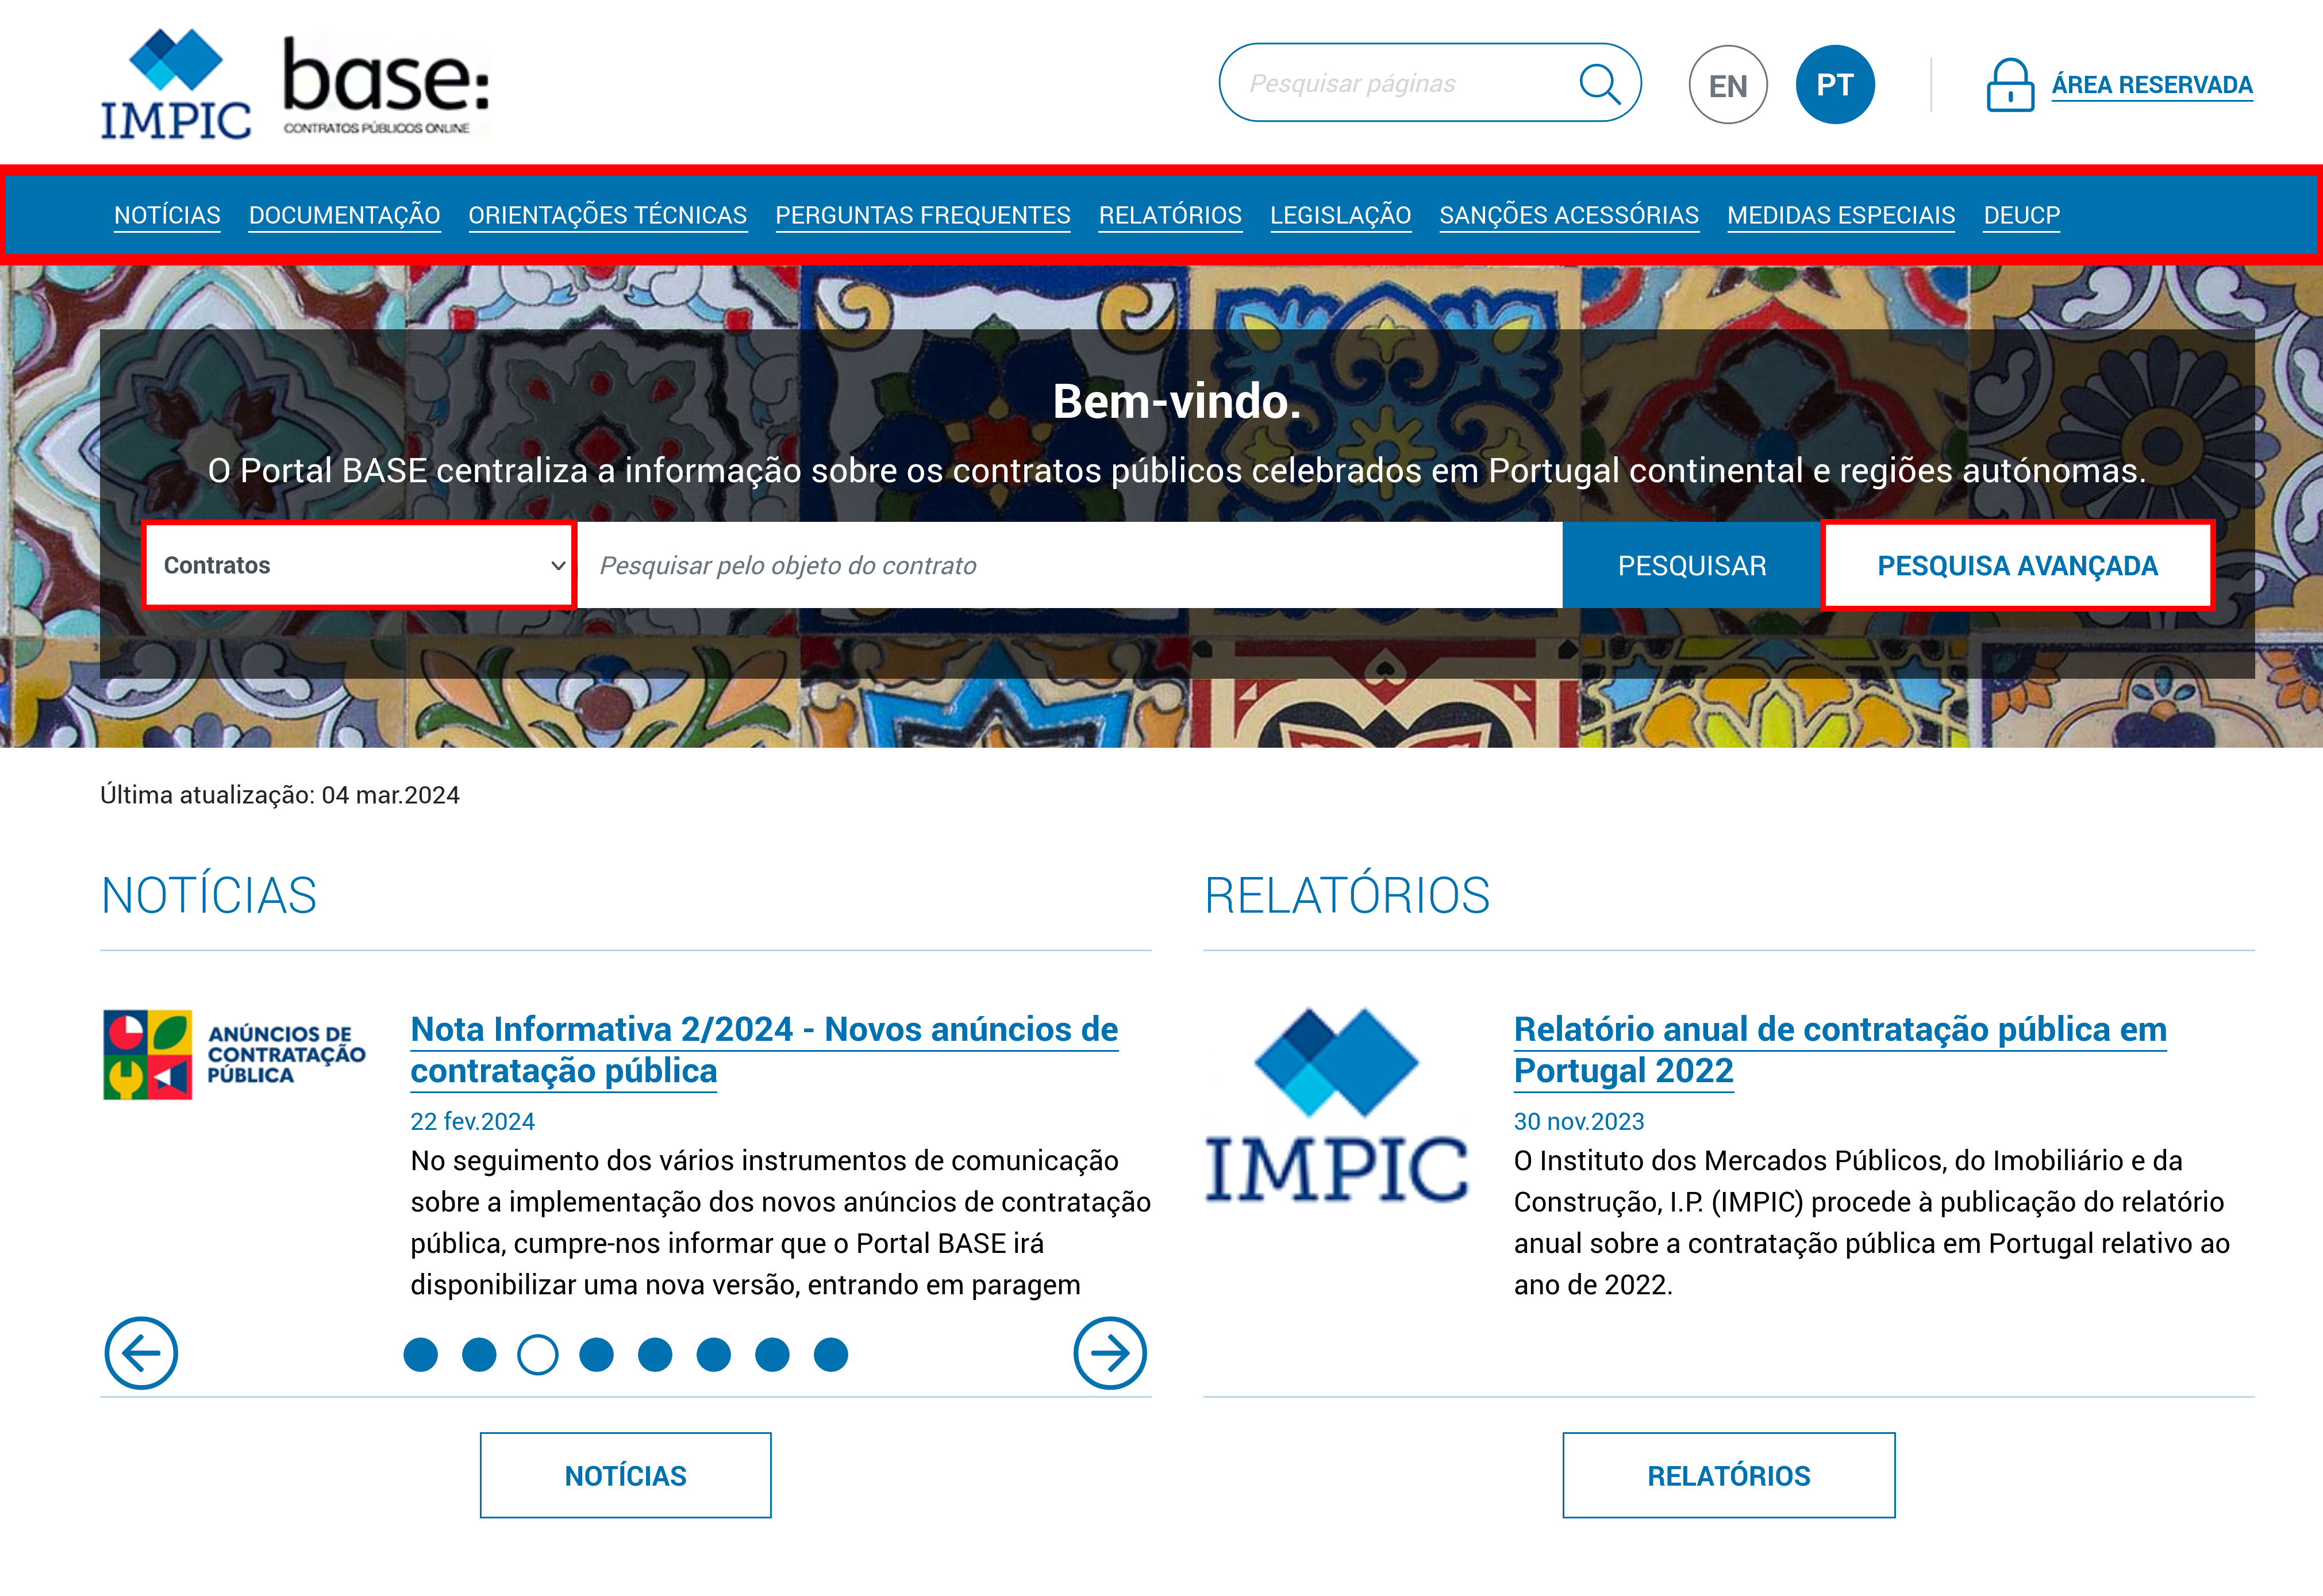
\includegraphics[width=\textwidth]{imagens/portalbase_init_v2.png}
	\caption{\textit{Screenshot} da página inicial do Portal BASE.}
	\label{fig:site1}
\end{figure}

\clearpage

\begin{figure}[H]
	\centering
	\includegraphics[width=\textwidth]{imagens/portalbase.png}
	\caption{\textit{Screenshot} do campo de pesquisa avançada do Portal BASE.}
	\label{fig:site2}
\end{figure}

Na Figura \ref{fig:site3} é possível verificar os últimos quatro contratos adicionados ao Portal BASE, no momento de captura de imagem do ecrã, dia 24 de abril de 2024. Para aceder às especificidades de cada um dos contratos é necessário pressionar o sinal \img{imagens/plus.png}, que se encontra delimitado a vermelho. A título de exemplo, identificam-se na Figura \ref{fig:site4} os detalhes contratuais do concurso público referente à contrução da nova linha de metro \textit{Rubi}, na cidade do Porto.

\begin{figure}[H]
	\centering
	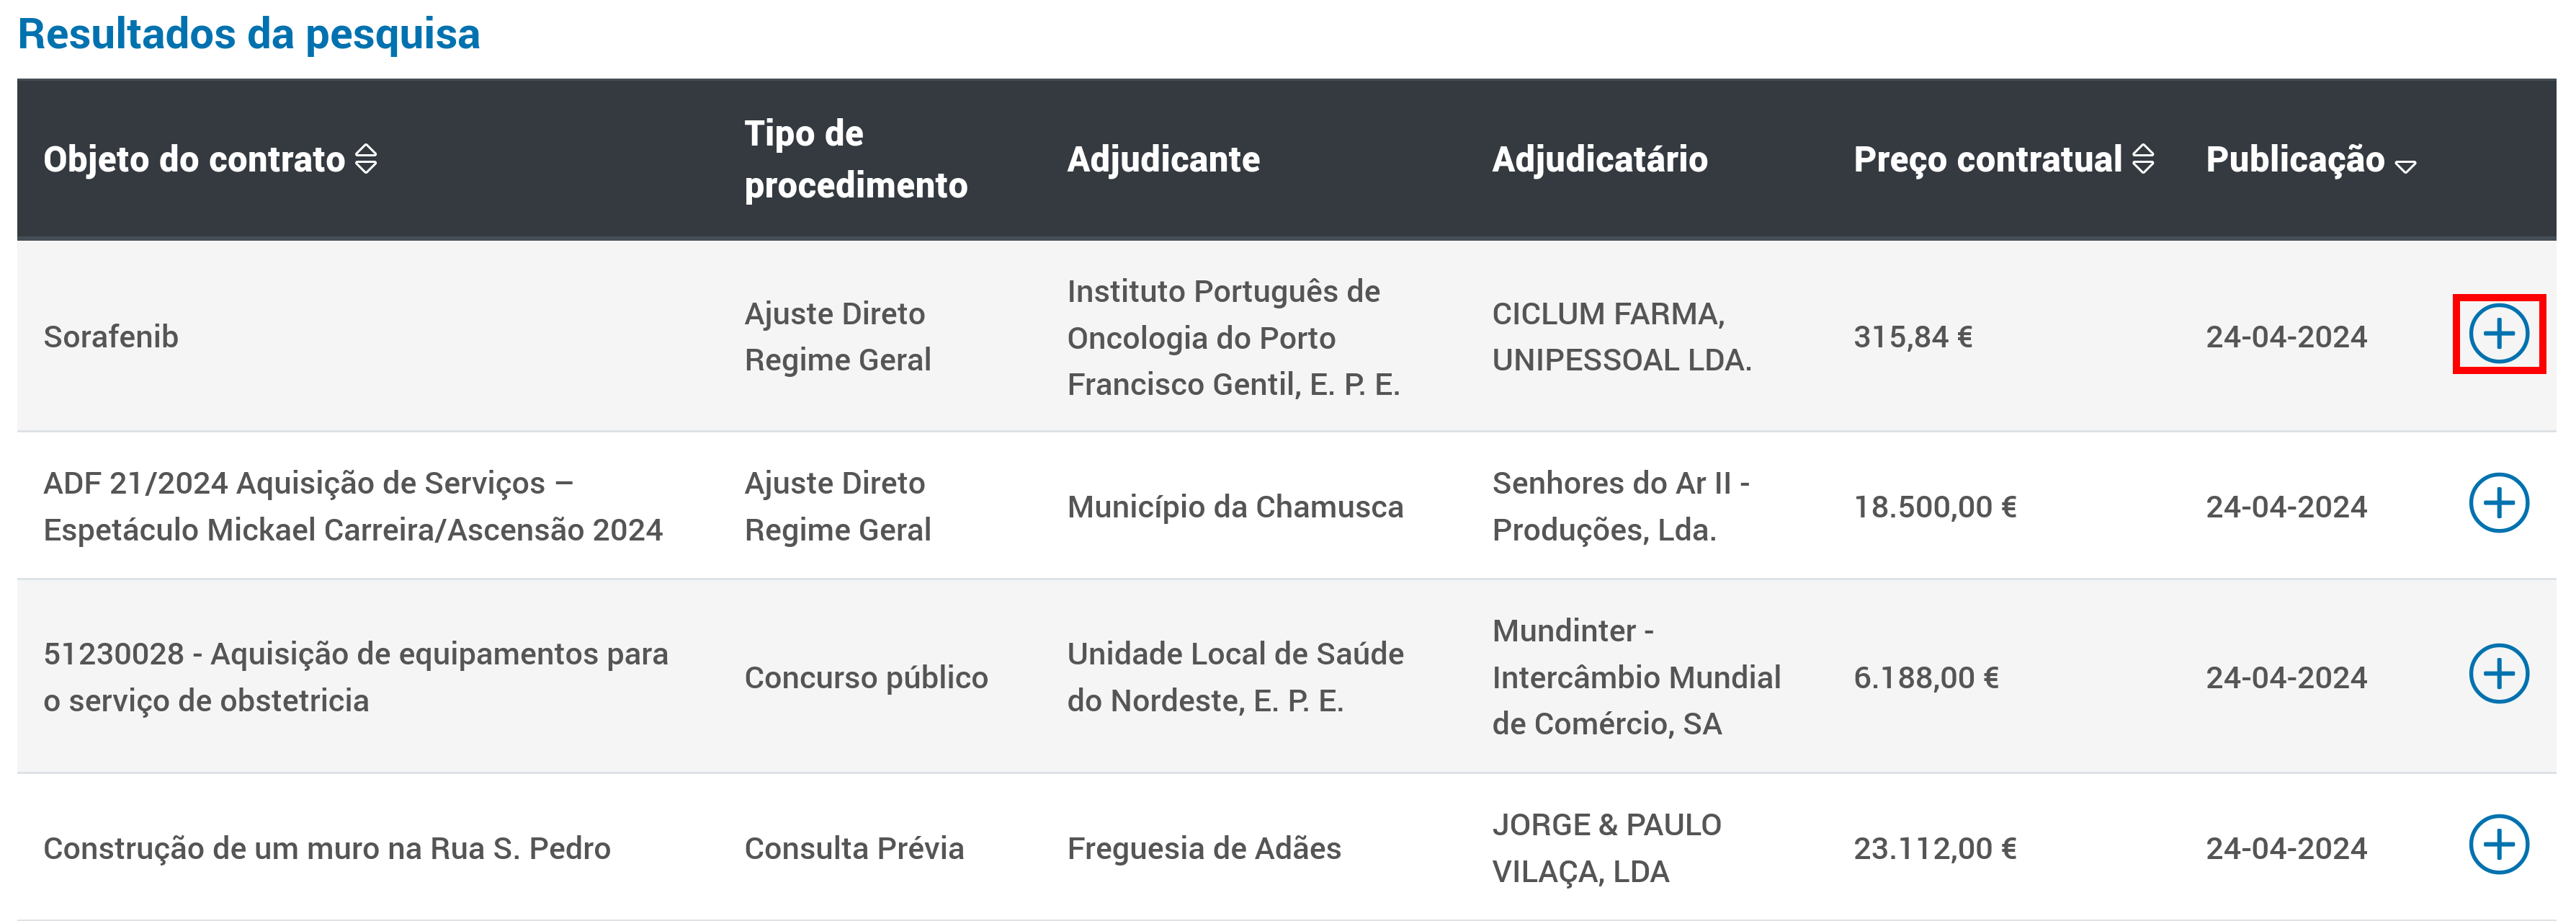
\includegraphics[width=\textwidth]{imagens/portalbase_pesquisa.png}
	\caption{\textit{Screenshot} dos últimos quatro contratos adicionados ao Portal BASE.}
	\label{fig:site3}
\end{figure}

\clearpage
\begin{figure}[H]
	\centering
	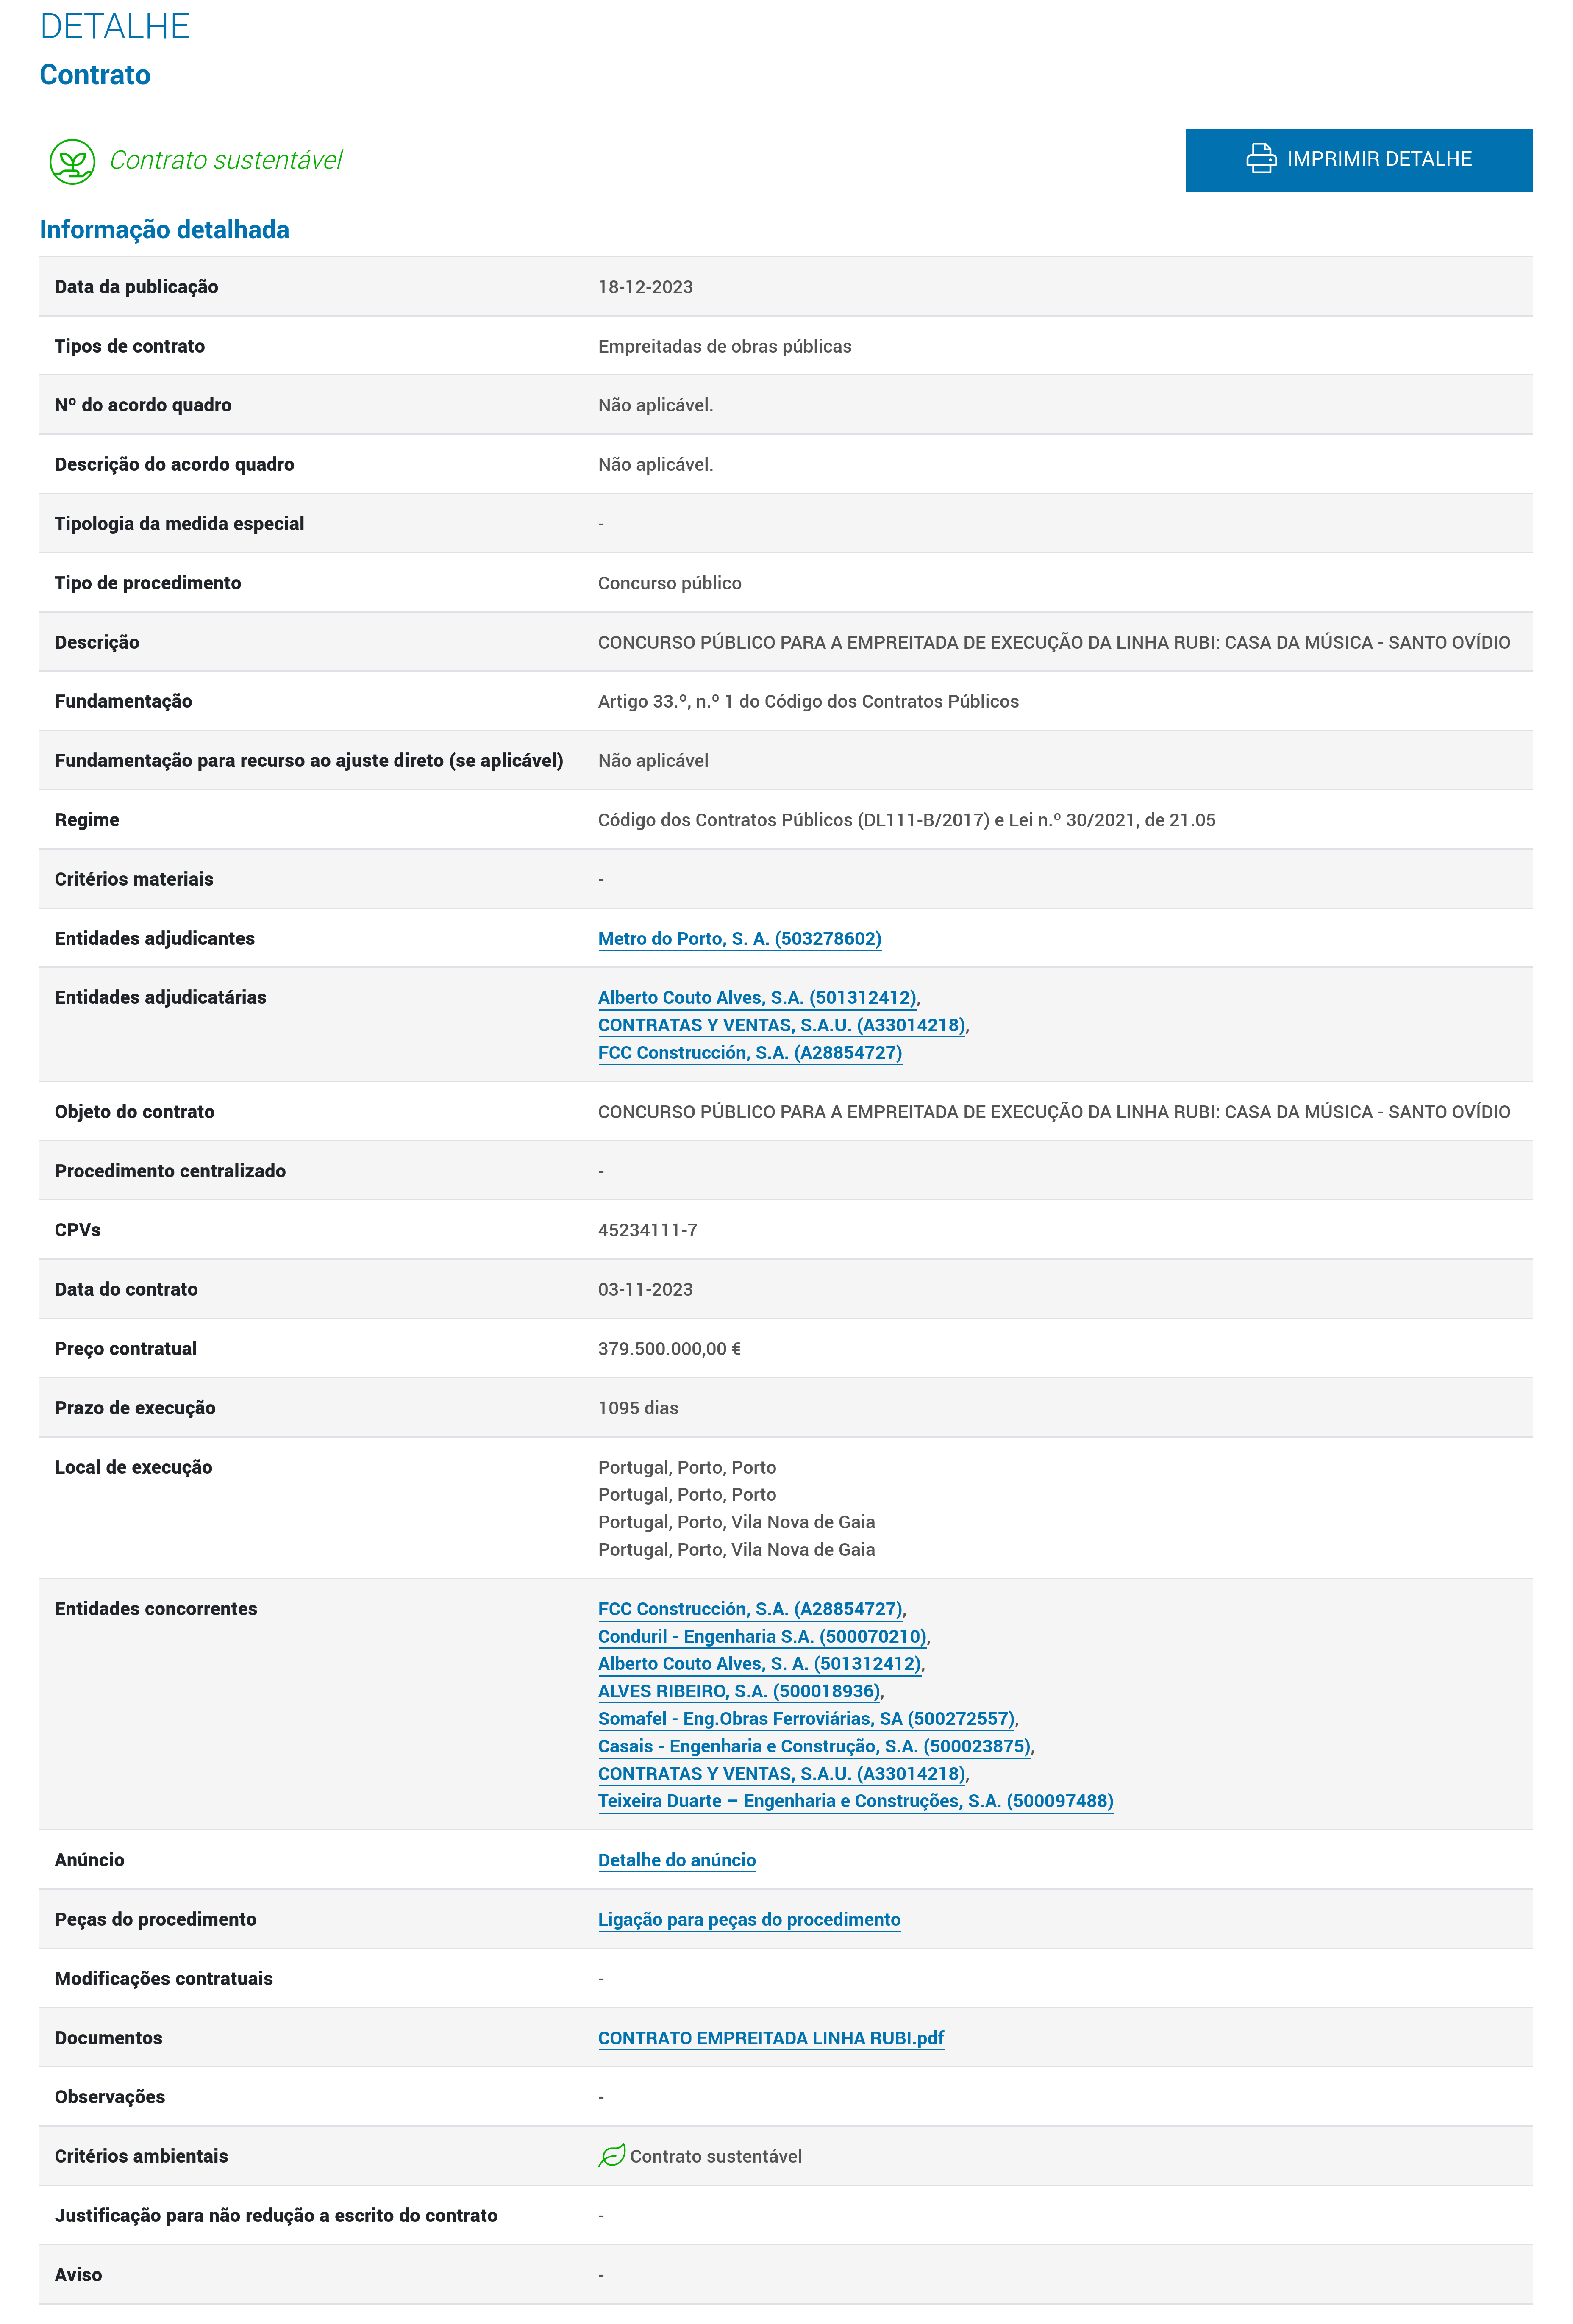
\includegraphics[width=\textwidth]{imagens/metro.png}
	\caption{\textit{Screenshot} dos detalhes do contrato referentes à contrução da Linha Rubi, do Metro do Porto.}
	\label{fig:site4}
\end{figure}

\clearpage
\subsection{Entidades envolvidas}

Existem diversas entidades que suportam o processo de contratação pública em Portugal. 

%\begin{figure}[h]
%	\centering
%	\begin{minipage}{.25\textwidth}
%		\centering
%		
\includegraphics[width=\linewidth]{imagens/ESPAP.png}
%	\end{minipage}%
%	\begin{minipage}{.25\textwidth}
%		\centering
%		
\includegraphics[scale = 0.1]{imagens/impic.jpg}
%	\end{minipage}%
%	\begin{minipage}{.25\textwidth}
%		\centering
%		
\includegraphics[width=\linewidth]{imagens/incm.png}
%	\end{minipage}%
%	\begin{minipage}{.25\textwidth}
%		\centering
%		
\includegraphics[width=.7\linewidth]{imagens/gns.png}
%	\end{minipage}
%	\caption{Entidades envolvidas no processo contratação pública}
%\end{figure}


\begin{my_enumerate}
	\item  \textbf{Instituto dos Mercados Públicos, do Imobiliário e da Construção, I.P. (IMPIC)}: É a entidade responsável por gerir o Portal BASE, monitorizar e fiscalizar as plataformas eletrónicas de contratação pública, regular os contratos públicos e assume-se como elo de ligação com a Comissão Europeia, para efeitos do disposto no nº 5, do artigo.º 83, da Diretiva nº 2014/24/EU. É responsável pelo desenvolvimento de manuais de boas práticas sobre contratos públicos de aquisição de obras, de bens e de prestação de serviços. Compete-lhe, ainda, a analise de queixas e denúncias de cidadãos e empresas.
	
	\item \textbf{Entidade de Serviços Partilhados da Administração Pública, I.P. (eSPap)}: É a entidade que desenvolve e presta serviços no âmbito da Administração Pública. Além disso, concebe, gere e avalia o sistema nacional de compras e assegura a gestão do PArque de Veículos do Estado (PVE), apoiando a definição de políticas estratégicas nas áreas das tecnologias de informação e comunicação (TIC) do Ministério das Finanças, garantindo o planeamento, conceção, execução e avaliação das iniciativas de informatização tecnológica dos respetivos serviços e organismos.
	
	\item \textbf{Gabinete Nacional de Segurança (GNS)}: É o organismo que garante a segurança da informação classificada de âmbito nacional e das organizações internacionais de que Portugal faz parte. É responsável por credenciar as plataformas eletrónicas de contratação pública, dos auditores de segurança, de pessoas e empresas para o acesso e manuseamento de informação classificada e entidades que atuem no âmbito do Sistema de Certificação Eletrónica do Estado - Infra-Estrutura de Chaves Públicas (SCEE).
	
	\item \textbf{Imprensa Nacional – Casa da Moeda (INCM)}: É a entidade responsável pelas publicações no Diário da República Eletrónico e no Jornal Oficial da União Europeia. Todos os anúncios dos procedimentos pré-contratuais (Concurso Público, Concurso Limitado por Prévia Qualificação, Procedimento de Negociação, Diálogo Concorrencial e Parceria para a Inovação) são publicados no Diário da República Eletrónico e, simultaneamente, publicitados no Portal BASE (excetuam-se os casos de ajuste direto e consulta prévia).
	
	\item \textbf{Entidades Adjudicantes}: São estas que conduzem e decidem o procedimento de formação de contrato e são responsáveis por introduzir, no Portal, informação sobre os contratos públicos celebrados. 
	
	\item \textbf{Adjudicatário}: Titular da proposta vencedora. Tem de comprovar que respeita os requisitos exigidos para poder celebrar o contrato. A informação é submetida no Portal BASE via plataforma eletrónica.
	
	\item \textbf{Plataforma Eletrónica}: É a infraestrutura tecnológica constituída por um conjunto de aplicações, meios e serviços informáticos onde, de forma totalmente eletrónica e desmaterializada, decorre a tramitação dos procedimentos para a formação de um contrato público. 
	
\end{my_enumerate}







\section{Descrição da Base de Dados}
\label{ch:variables}


O conjunto de dados contratuais disponibilizado e utilizado ao longo deste projeto encontra-se armazenado numa base de dados, em PostgreSQL. Salvo raras exceções, são adicionados ao Portal BASE, com caráter diário, os mais recentes contratos celebrados. Além disso, diariamente, são adicionados à base de dados todos os novos contratos do dia anterior, havendo, por isso, um desfasamento de um dia de forma a garantir que todos eles são coletados. 


\begin{figure}[H]
	\centering
	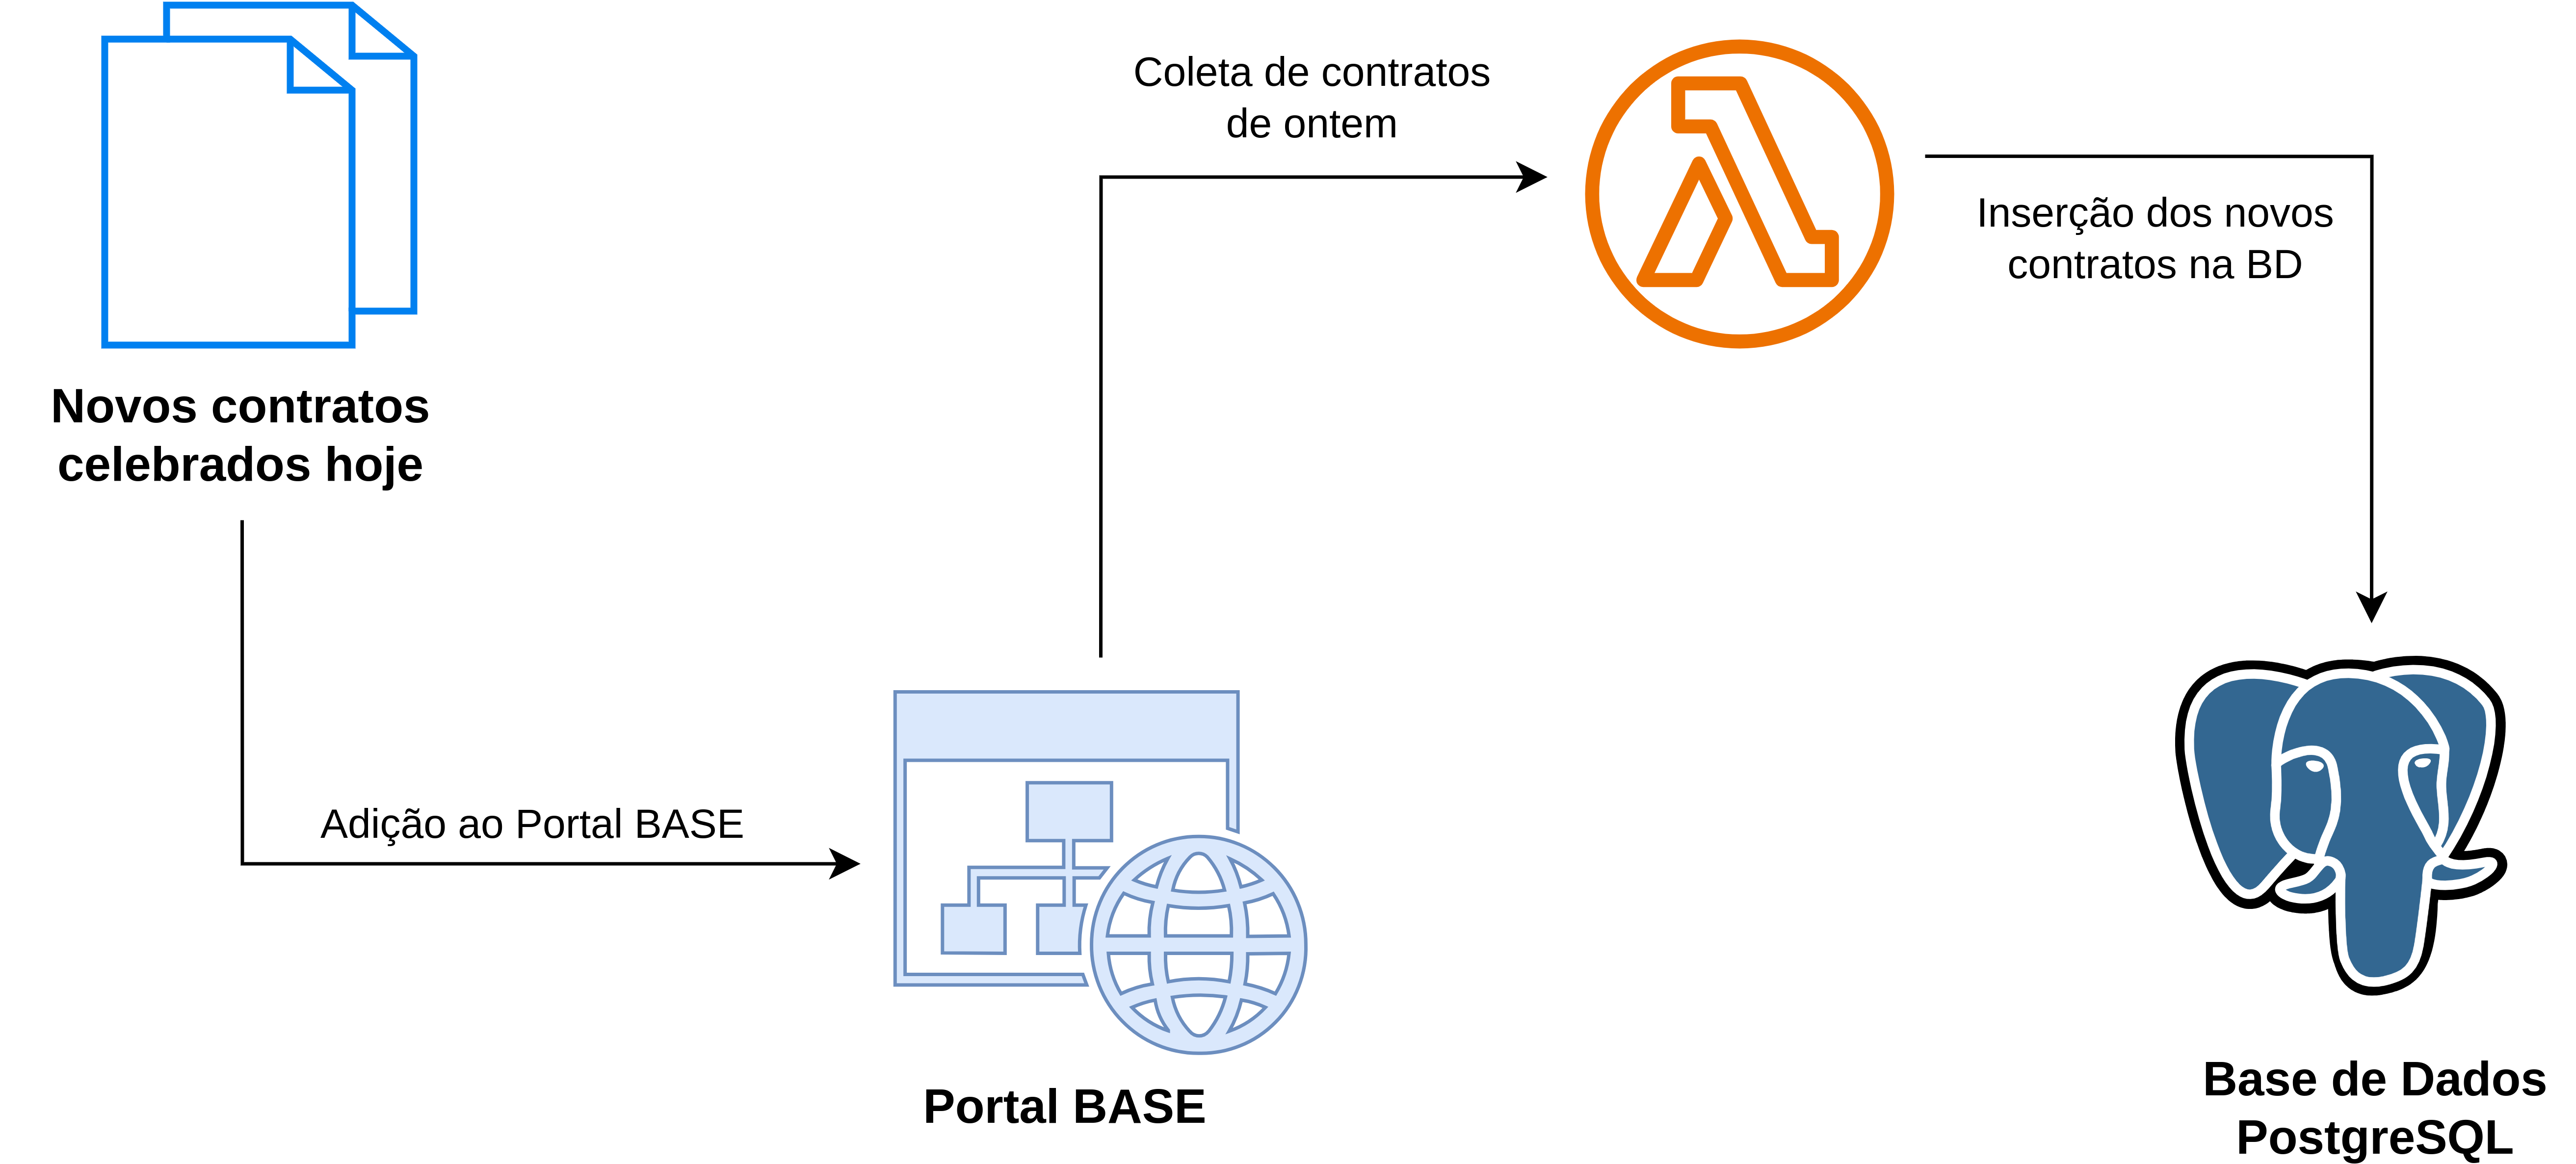
\includegraphics[width=0.7\textwidth]{imagens/portal_coleta.png}
	\caption{Processo de coleta de contratos e construção da base de dados.}
	\label{fig:processocoleta}
\end{figure}


Até ao primeiro dia do mês de maio, do presente ano civil, o conjunto de dados totalizava 1023443 contratos públicos, celebrados desde o dia 13 de maio de 2003. No trabalho que ora se apresenta, apenas foram considerados os contratos celebrados entre o dia 1 de janeiro de 2018 e o dia 1 de maio de 2024. Por assim ser, o número de contratos relativos ao ano de 2024 encontra-se incompleto. Pelo que, nas representações gráficas presentes nas secções que se seguem, a etiqueta relativa ao ano de 2024 será assinalada como \textbf{2024*}, a fim de sinalizar o facto de o conjunto não estar completo para o presente ano civil. 

Do total das 61 colunas da base de dados onde se encontram guardados todos os contratos públicos, as que reveleram maior interesse foram as seguintes: 


\begin{my_itemize}
	

\item \textbf{id} (integer): É o número que permite identificar um contrato específico na base de dados. A cada contrato foi atribuído um identificador único.


\item \textbf{n\_anuncio} (text): O número de anúncio é o número que permite identificar o anúncio no Diário da República Digital, referente a um determinado procedimento de contratação pública.


\item \textbf{anuncio\_preco\_base} (float): O preço base é definido como o preço máximo que a entidade adjudicante está disposta a pagar pela execução de todas as prestações que constituem o objeto do contrato a celebrar.


\item \textbf{anuncio\_proposalDeadline} (date): Este campo diz respeito ao número de dias estipulado para submeter uma proposta a um determinado concurso, por parte de uma entidade concorrente. 


\item \textbf{tipo\_procedimento} (text): Este parâmetro permite identificar o tipo de procedimento, de acordo com os enunciados na tabela \ref{table:2}, de um  determinado contrato público.


\item \textbf{objeto\_contrato} (text): O objeto de contrato consiste numa descrição detalhada do tipo de objeto celebrado. 


\item \textbf{data\_publicacao} (date): Este parâmetro diz respeito à data de publicação do contrato no Portal BASE.


\item \textbf{data\_celebracao} (date): Este parâmetro diz respeito à data de celebração do contrato. 

\item \textbf{preco\_contratual} (float): O  preço contratual é o preço a pagar pela entidade adjudicante à entidade vencedora após celebração do objeto contratual. 

\item \textbf{entidade\_adjudicante} (text): Este campo contém o nome, número de identificação fiscal e URL que remete para a página \textit{website} do Portal BASE com todos os contratos celebrados de uma determinada entidade adjudicante. 

\begin{figure}[H]
	\centering
	
\includegraphics[width=.9\textwidth]{imagens/adjudicante.png}
	\caption{Exemplo de uma entidade adjudicante de um contrato presente na base de dados.}
	\label{fig:adjudicante}
\end{figure}

\item \textbf{fundamentacao} (text): A fundamentação diz respeito ao artigo do CCP utilizado para justificar a adoção do procedimento escolhido. 

\item \textbf{entidades\_contratadas} (text): À semelhança do campo \textbf{entidade\_adjudicante}, este campo contém o nome, número de identificação fiscal e URL que remete para a página \textit{web} do Portal BASE com todos os contratos celebrados de uma determinada entidade adjudicatária. 

\item \textbf{entidades\_concorrentes} (text): Neste campo é possível encontrar o nome, número de identificação fiscal e URL que remete para o \textit{website} do Portal BASE com todos os contratos celebrados para todas as entidades que concorrem a um determinado contrato público. Quando existe mais do que uma entidade concorrente, a separação entre entidades é feita através dos caracteres \(|||\).



\begin{figure}[H]
	\centering
	
\includegraphics[width=.9\textwidth]{imagens/concorrentes.png}
	\caption{Exemplo de entidades concorrentes de um contrato presente na base de dados.}
	\label{fig:concorrentes}
\end{figure}


\item \textbf{url\_anuncio} (text): Contém um \textit{link} que redireciona para a página \textit{web} que contém os detalhes do anúncio.

\item \textbf{cpv} (text): Contém o CPV do contrato. CPV é a sigla de \textit{Common Procurement Vocabulary}. O CPV é um código de oito dígitos, usado no processo de contratação, que permite especificar e categorizar de forma hierárquica serviços e produtos. 

\begin{my_itemize}
	\item[$\circ$] \label{sec:cepeves}  Os 2 primeiros dígitos permitem identificar a \textbf{divisão} do serviço/produto. No total, existem 45 divisões.
	\item[$\circ$]  Os 3 primeiros dígitos permitem identificar o \textbf{grupo}. No total, existem 272 grupos.
	\item[$\circ$]  Os 4 primeiros dígitos permitem identificar a \textbf{classe}. No total, existem, 1002 classes.
	\item[$\circ$]  Os 5 primeiros dígitos permitem identificar a \textbf{categoria}. No total, existem 2379 categorias.
	\item[$\circ$]  Os 6 primeiros dígitos permitem identificar a \textbf{subcategoria}. No total, existem 5756 subcategorias.
\end{my_itemize}

A título de exemplo, atente-se no caso seguinte caso:

\begin{figure}[H]
	\centering
	
\includegraphics[width=0.7\textwidth]{imagens/cpv.png}
	\caption{Ilustração do CPV de um contrato referente a veículos de combate a incêndios.}
	\label{fig:cpv}
\end{figure}


\begin{my_itemize}
	\item[$\circ$]  \textbf{Divisão:} 34 - Equipamentos de transporte e produtos auxiliares ao transporte
	\item[$\circ$]  \textbf{Grupo:} 341 - Veículos motorizados
	\item[$\circ$]  \textbf{Classe:} 3414 - Veículos motorizados pesados
	\item[$\circ$]  \textbf{Categoria:} 34144 - Veículos motorizados para fins especiais
	\item[$\circ$]  \textbf{Subcategoria:} 34144210 - Veículos de combate a incêndios
\end{my_itemize}



\item \textbf{contractType} (text): Este campo diz respeito ao tipo de contrato celebrado, tal como se encontra apresentado Tabela \ref{table:3}. 

\item \textbf{executionPlace} (text): Indica o local de execução do contrato. 

\item \textbf{totalEffectivePrice} (float): Na eventualidade de existirem alterações do preço contratual após a celebração do contrato, este campo é preenchido. Existem, também, casos em que o preço contratual diz respeito à unidade em questão (p. ex. quilómetro, hora, dia). Nessa situação, o preço total efetivo é o preço total após prestação do serviço \cite{jardinagem}.  

\end{my_itemize}

De entre o universo de contratos celebrados, pode-se perceber na Tabela \ref{tab:contratos} como estes se distribuem consoante os diferentes tipos de procedimentos. Como se pode verificar, os tipos de procedimentos com maior relevância são: o Ajuste Direto em Regime Geral, a Consulta Prévia, o Concurso Público e contratos ao abrigo de acordo-quadro, com especial evidência para o Ajuste Direto em Regime Geral que prefaz 50\% dos contratos. 


\begin{table}[H]
	\centering
	\renewcommand{\arraystretch}{1.15}
	\setlength{\tabcolsep}{15pt}
	\resizebox{\textwidth}{!}} \\ \hline
			Ajuste Direto Regime Geral                                                     & 526860                                                                   & 51.4                                                            \\ \hline
			\rowcolor[HTML]{EFEFEF} 
			Consulta Prévia                                                                & 228400                                                                   & 22.3                                                            \\ \hline
			Concurso público                                                               & 128422                                                                   & 12.5                                                            \\ \hline
			\rowcolor[HTML]{EFEFEF} 
			Ao abrigo de acordo-quadro (art.º 259.º)                                       & 111723                                                                   & 10.9                                                            \\ \hline
			Ao abrigo de acordo-quadro (art.º 258.º)                                       & 24406                                                                    & 2.4                                                             \\ \hline
			Concurso limitado por prévia qualificação                                      & 1816                                                                     & $< 1$                                                            \\ \hline
			\rowcolor[HTML]{EFEFEF} 
			Consulta Prévia Simplificada                                                   & 958                                                                      & $< 1$                                                            \\ \hline
			Contratação excluída II                                                        & 485                                                                      & $< 1$                                                            \\ \hline
			Setores especiais – isenção parte II                                           & 222                                                                      & $< 1$                                                          \\ \hline
			\rowcolor[HTML]{EFEFEF} 
			Procedimento de negociação                                                     & 45                                                                       & $< 1$                                                          \\ \hline
			Concurso público simplificado                                                  & 42                                                                       & $< 1$                                                          \\ \hline
			\rowcolor[HTML]{EFEFEF} 
			Consulta prévia ao abrigo do artigo 7º da Lei n.º 30/2021, de 21.05            & 25                                                                       & $< 1$                                                          \\ \hline
			Ajuste Direto Regime Geral ao abrigo do artigo 7º da Lei n.º 30/2021, de 21.05 & 21                                                                       & $< 1$                                                          \\ \hline
			\rowcolor[HTML]{EFEFEF} 
			Serviços sociais e outros serviços específicos                                 & 9                                                                        & $< 1$                                                          \\ \hline
			Concurso de conceção simplificado                                              & 4                                                                        & $< 1$                                                          \\ \hline
		\end{tabular}%
	}
	\caption{Número de contratos públicos e respetiva fração para os vários tipos de procedimentos.}
	\label{tab:contratos}	
\end{table}



%\rowcolor[HTML]{EFEFEF} 
%Parceria para a inovação                                                       & 2                                                                        & $< 1$                                                          \\ \hline
%Concurso de ideias simplificado                                                & 1                                                                        & $< 1$                                                          \\ \hline
%\rowcolor[HTML]{EFEFEF} 
%Não especificado & 1                                                                        & $< 1$                                                           \\ \hline



A leitura das Figuras \ref{fig:numcontrs} e \ref{fig:precoscontrs} permite inferir uma tendência crescente do número de contratos celebrados entre 2018 e 2023, estando este comportamento em linha com o crescimento do preço contratual total por ano. 

\begin{figure}[H]
	\centering
	\begin{minipage}{.49\linewidth}
		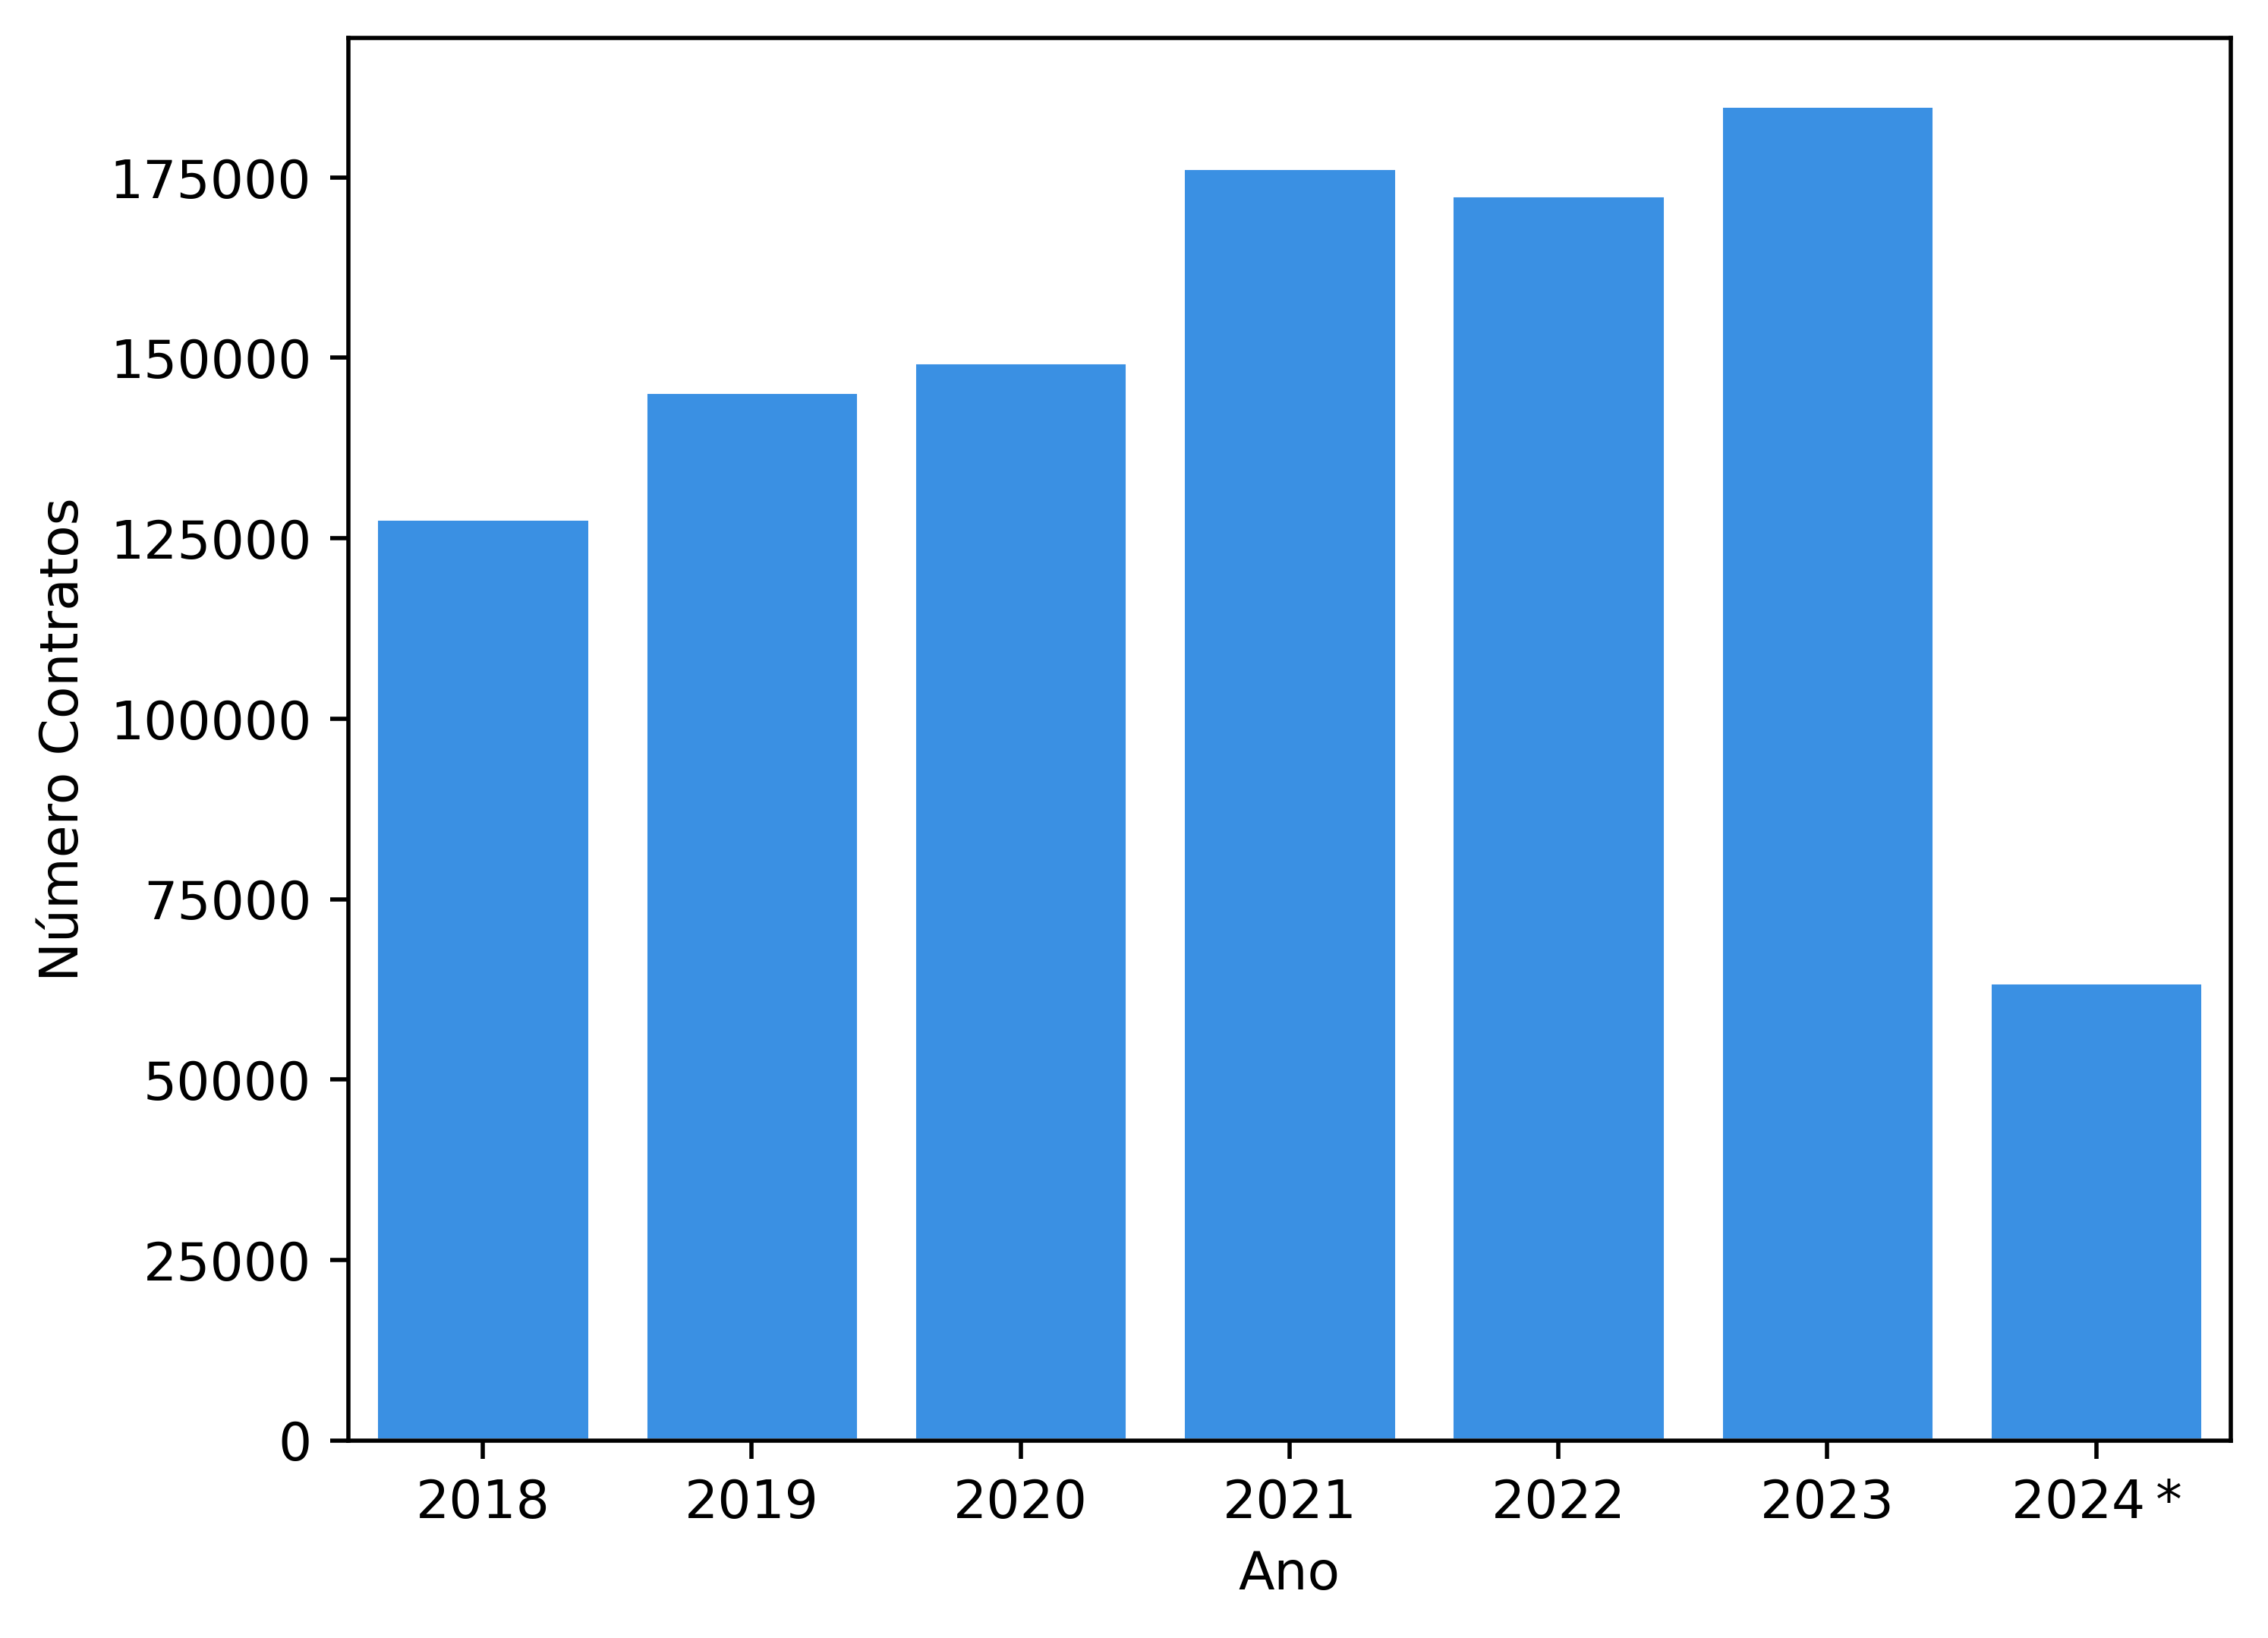
\includegraphics[width=\linewidth]{imagens/contratos_ano.png}
		\caption{Número de contratos celebrados, entre 2018 e 2024, para todas as tipologias.}
		\label{fig:numcontrs}
	\end{minipage}
	\hfill
	\begin{minipage}{.49\linewidth}
		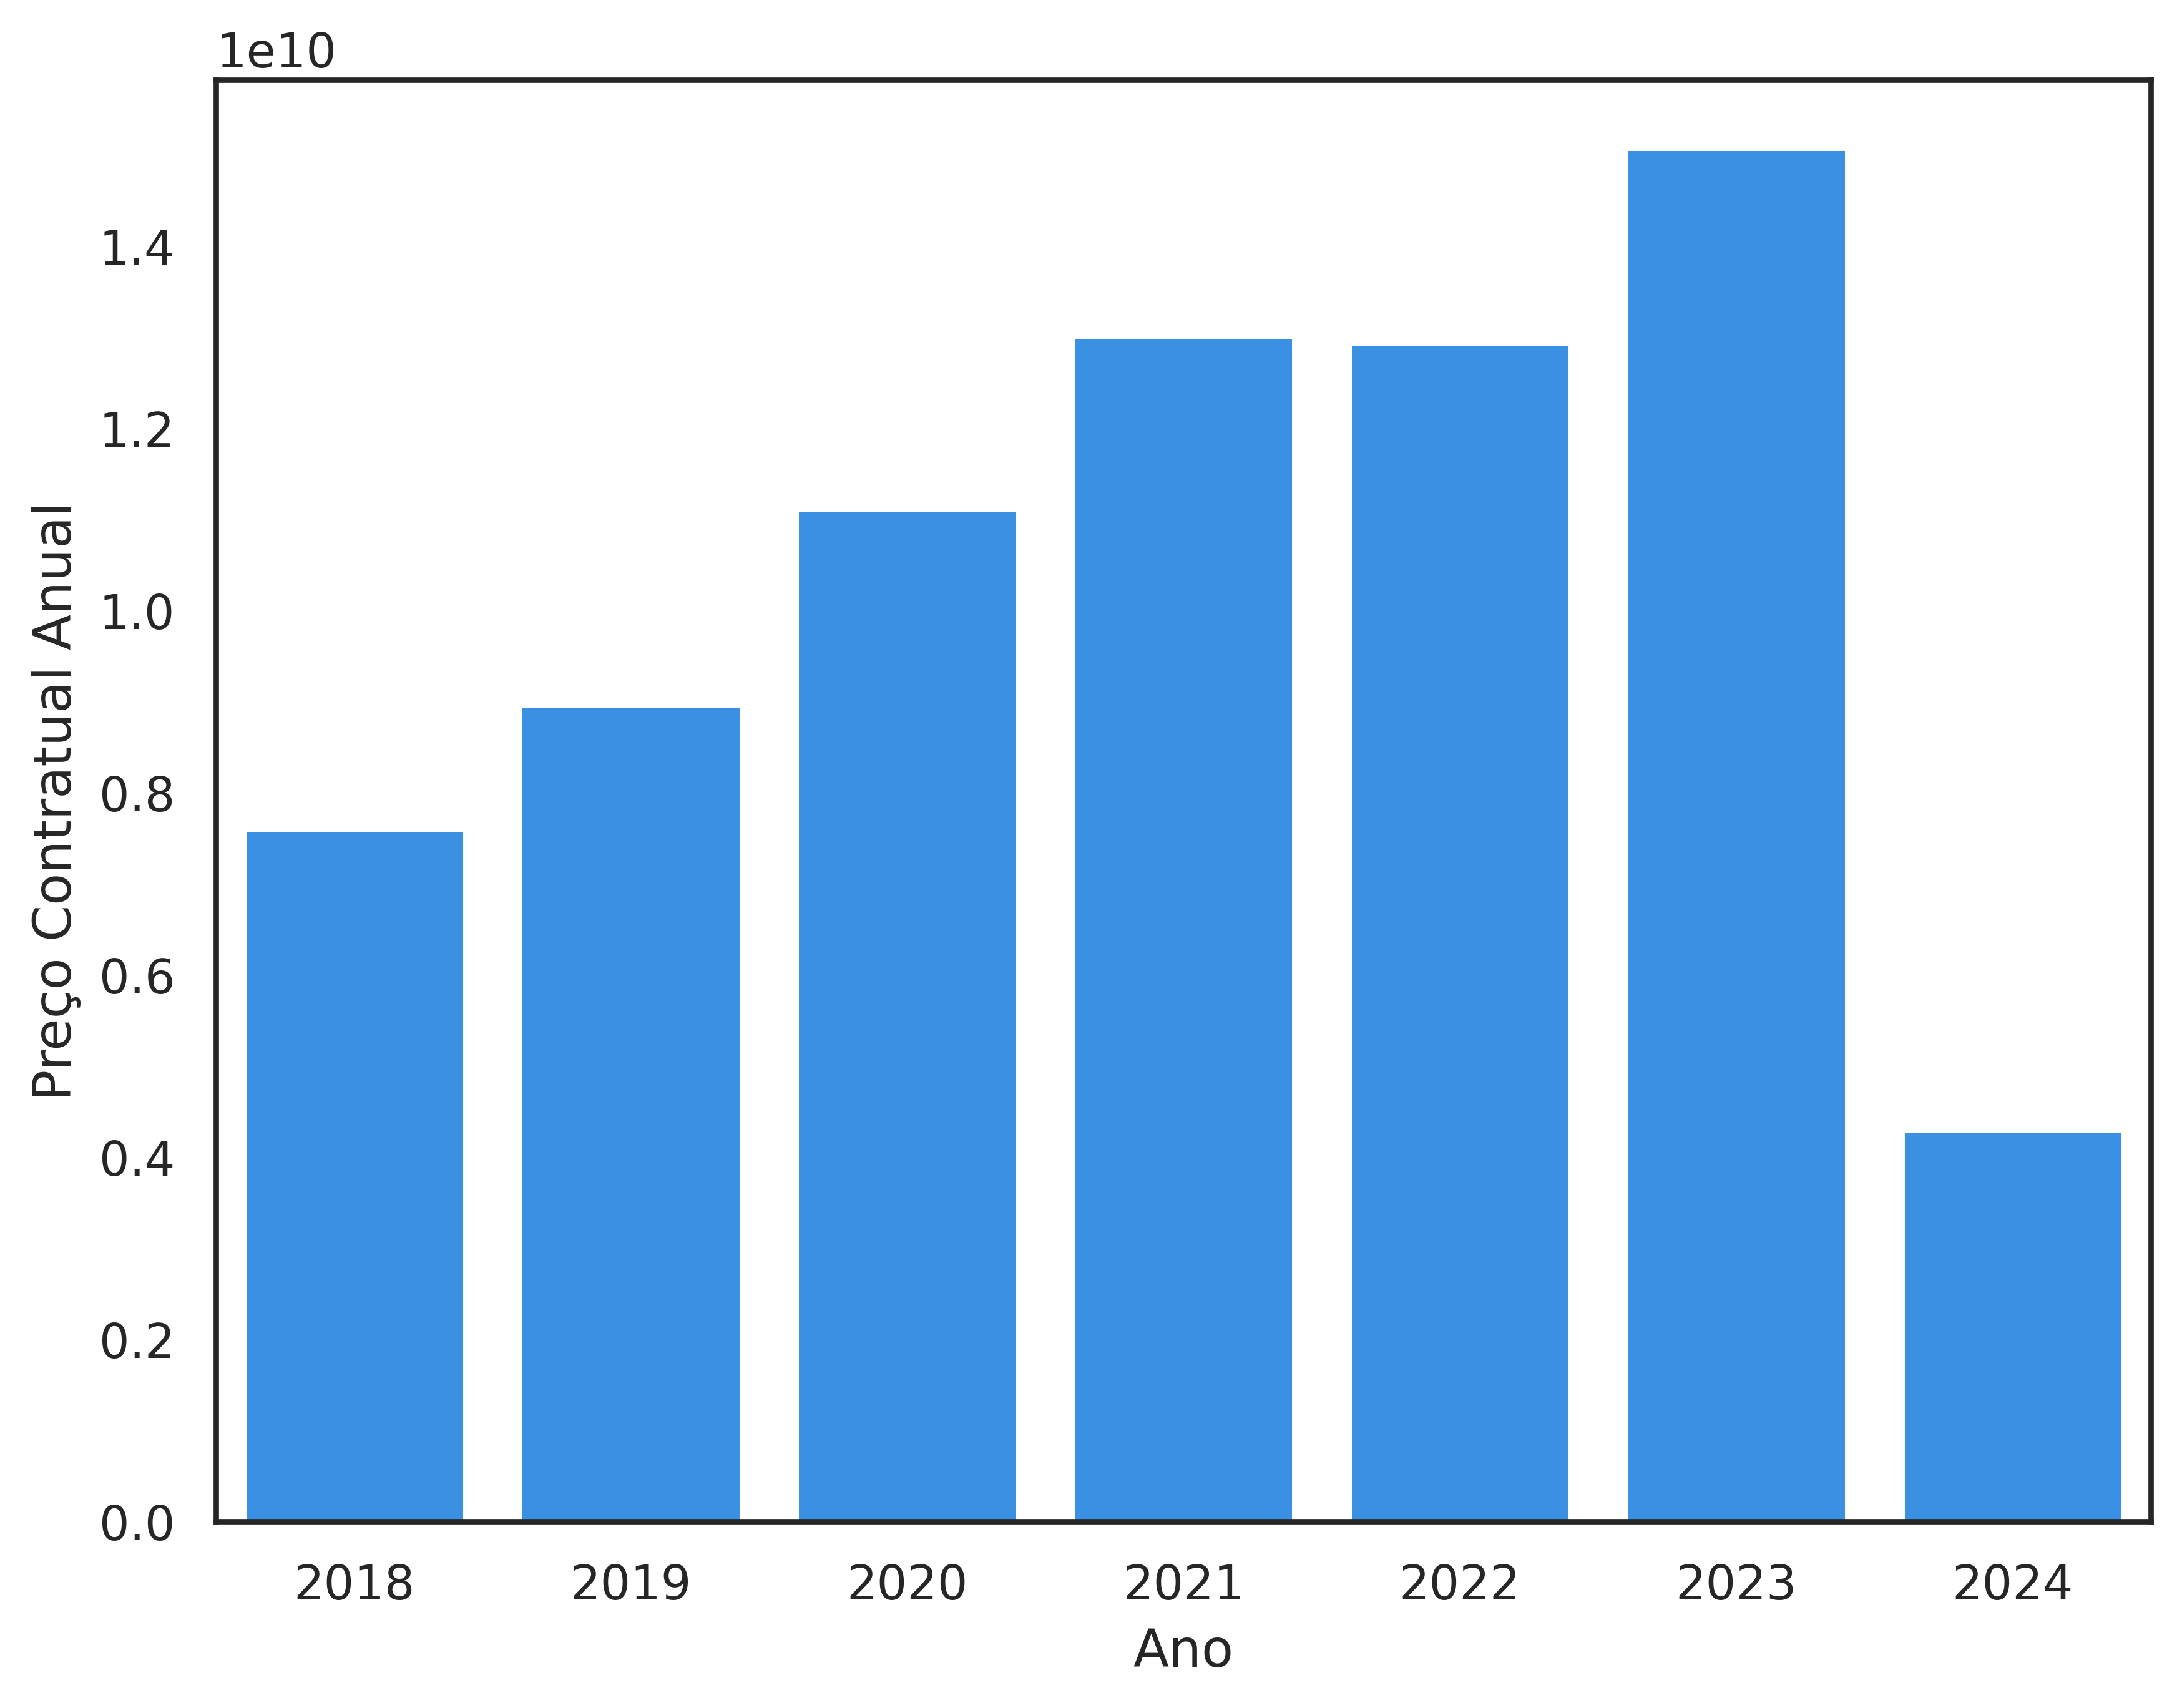
\includegraphics[width=\linewidth]{imagens/precocontr_ano.png}
		\caption{Preço contratual total, entre 2018 e 2024, para todas as tipologias}
		\label{fig:precoscontrs}
	\end{minipage}
\end{figure}


%\begin{wrapfigure}{R}{0.45\textwidth}
%	\centering
%	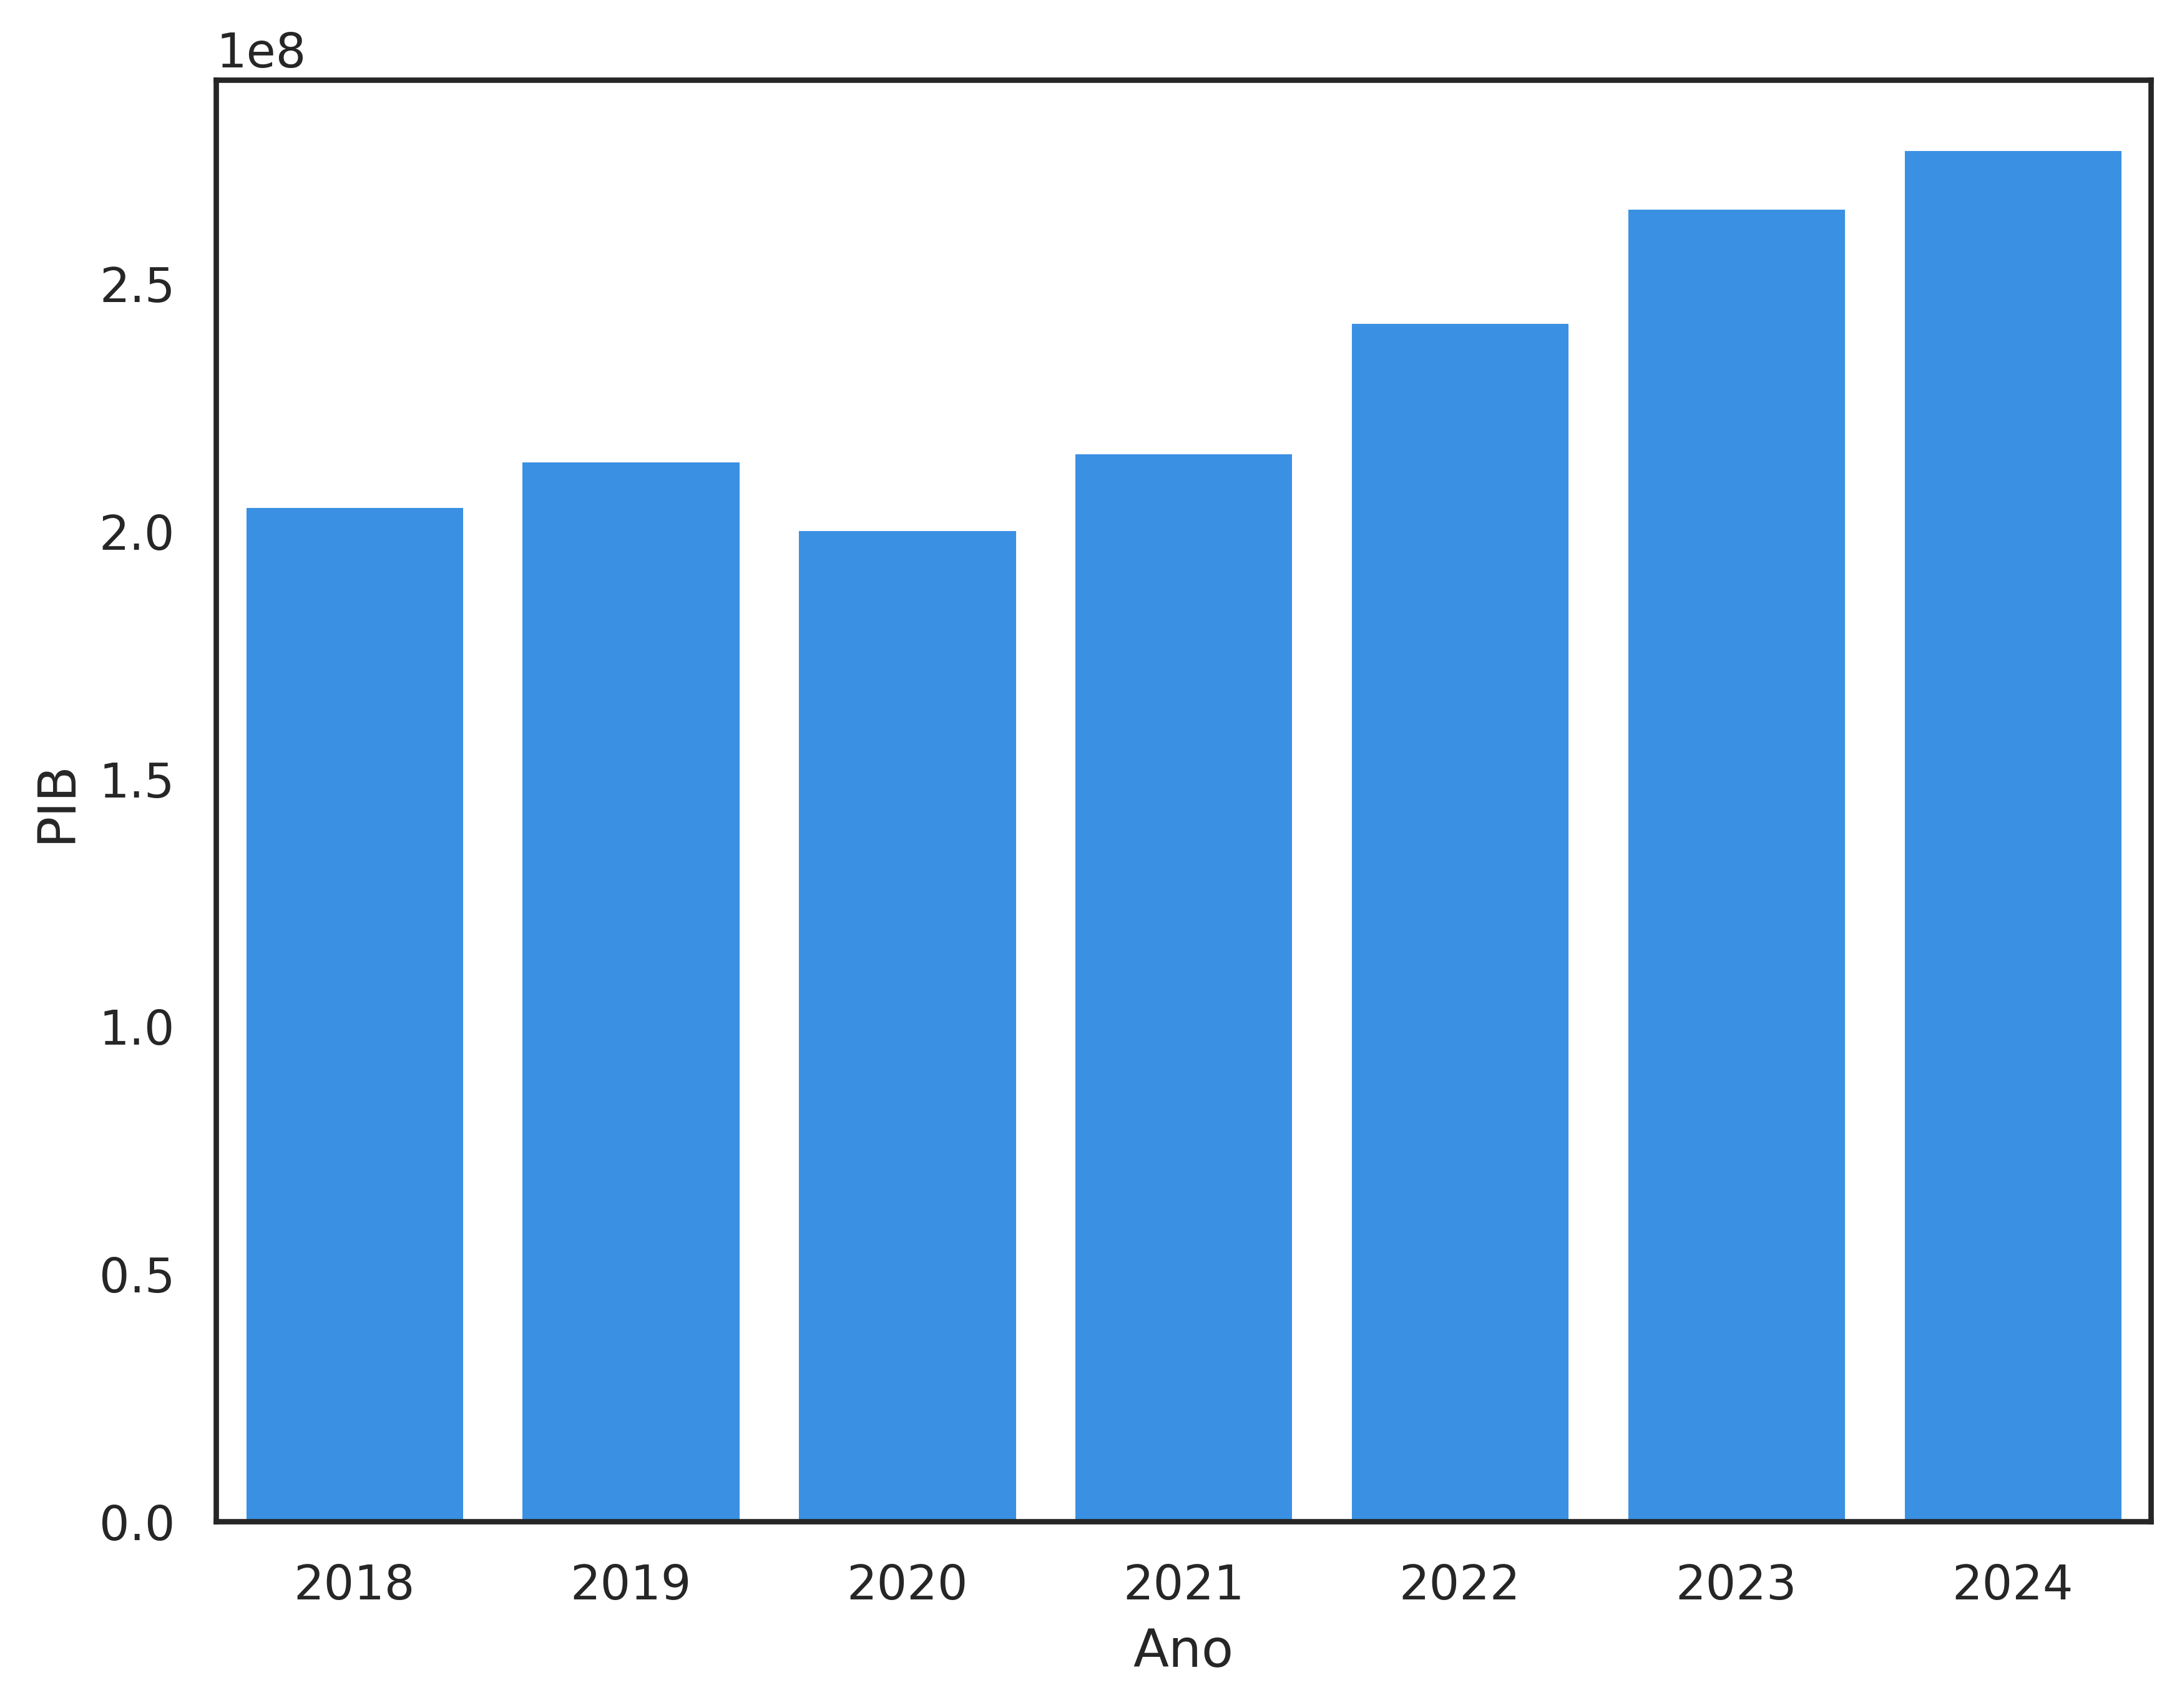
\includegraphics[width=0.45\textwidth]{imagens/pib.png}
%	\caption{PIB português entre 2018 e 2024}
%\end{wrapfigure}




\begin{table}[H]
	\centering
	\renewcommand{\arraystretch}{1.35}
	\setlength{\tabcolsep}{20pt}
	\resizebox{\textwidth}{!}{%
		\begin{tabular}{l|l}
			\textbf{33} & {\color[HTML]{000000} Equipamento médico, medicamentos, e produtos para cuidados pessoais}     \\
			\textbf{45} & Construção                                                                                     \\
			\textbf{79} & Serviços a empresas: direto, comercialização, consultoria, recrutamento, impressão e segurança \\
			\textbf{50} & Serviços de reparação e manuntenção                                                           
		\end{tabular}%
	}
	\caption{Descrição das principais divisões de CPV.}
	\label{tab:maincpvs}
\end{table}

Na Figura \ref{fig:distritos}, constata-se que existe uma prevalência de contratos celebrados nos distritos de Lisboa e do Porto, com 21\% e 14\%, respetivamente. Pelo contrário, nos distritos do interior esse valor aproxima-se dos 14\%. Existe, também, um elevado de número de contratos cujo distrito é identificado como \textit{Outro}. Estes casos, dizem respeito a erros de preenchimentos aquando da submissão dos contratos no Portal BASE, pois no campo \textbf{executionPlace} verificava-se um dos três cenários: o campo encontrava-se vazio, era inserido \textit{Distrito não determinado} ou era inserido \textit{Portugal Continental}. A partir da Figura \ref{fig:cpvs} observa-se que existe uma predominância de contratos públicos celebrados referentes à aquisição de equipamento médico, medicamentos e produtos para cuidados pessoais. Estes são todos os contratos cujos primeiros dois dígitos do CPV são 33. As quatro principais divisões do CPV, com maior número de contratos públicos celebrados, encontram-se na Tabela \ref{tab:maincpvs}. 

%\begin{table}[H]
%	\centering
%	\renewcommand{\arraystretch}{1.15}
%	\setlength{\tabcolsep}{15pt}
%	\resizebox{\textwidth}{!}{%
%		\begin{tabular}{ccccccccc}
%			\hline
%			\rowcolor[HTML]{C0C0C0} 
%			\textbf{Ano} & \textbf{Count} & \textbf{Média} & \textbf{D.Padrão} & \textbf{Min} & \textbf{Q1} & \textbf{Q2} & \textbf{Q3} & \textbf{Máx} \\ \hline
%			2024         & 90658          & 77953.18       & 1669717           & 0            & 3000        & 10800       & 29960.68    & 321888000    \\ \hline
%			\rowcolor[HTML]{EFEFEF} 
%			2023         & 191800         & 80514.25       & 1257076           & 0            & 4462.195    & 12005.18    & 33094.81    & 379500000    \\ \hline
%			2022         & 187193         & 66523.14       & 2106541           & 0            & 2250        & 9600.37     & 26260       & 881534700    \\ \hline
%			\rowcolor[HTML]{EFEFEF} 
%			2021         & 192112         & 71350.19       & 1723635           & 0            & 1564        & 8786.44     & 25560       & 397191000    \\ \hline
%			2020         & 164008         & 65710.67       & 804483.3          & 0            & 2280        & 9775.44     & 27763.44    & 130286000    \\ \hline
%			\rowcolor[HTML]{EFEFEF} 
%			2019         & 144769         & 61262.23       & 655422.8          & 0            & 3499        & 10682       & 28935       & 130463800    \\ \hline
%			2018         & 122089         & 58729.34       & 382421.9          & 0            & 4100        & 11458.2     & 30496.77    & 38750000     \\ \hline
%		\end{tabular}%
%	}
%	\caption{}
%	\label{tab:my-table}
%\end{table}



\clearpage
\vfill
\begin{figure}[H]
	\centering
	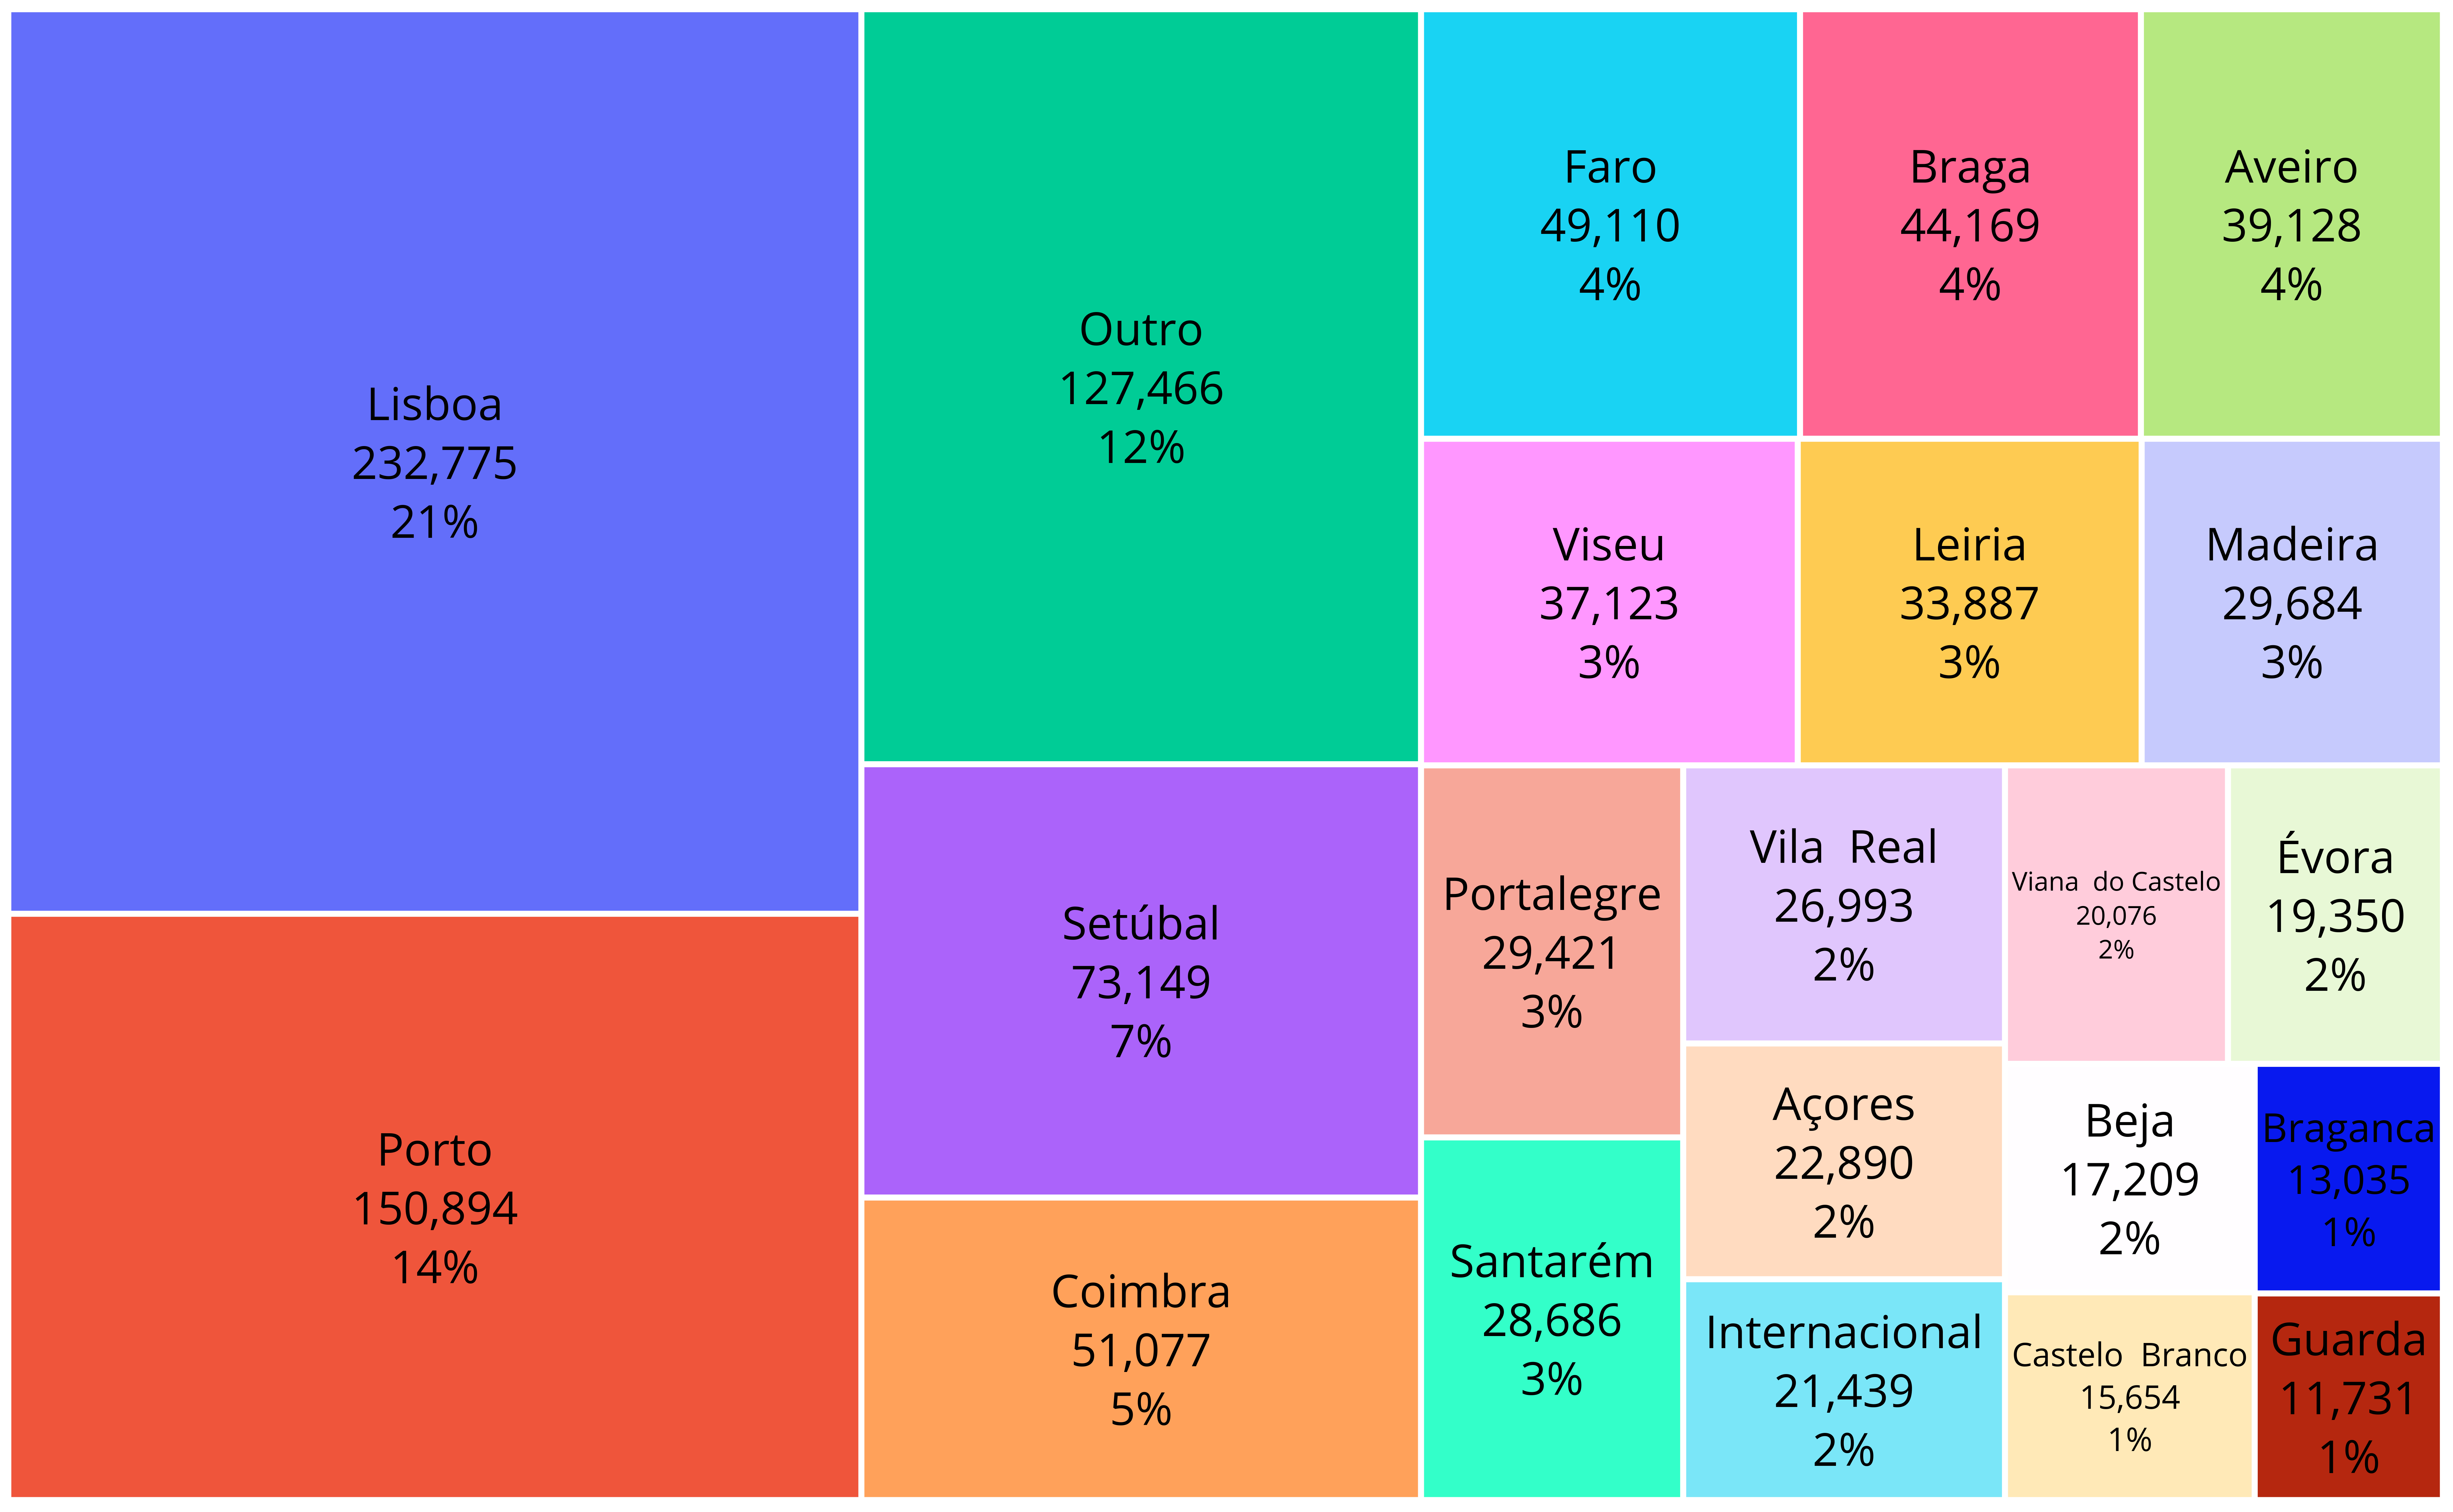
\includegraphics[width=\textwidth]{imagens/treemap_distritos.png}
	\caption{Distribuição do número de contratos públicos, por distrito, em Portugal.}
	\label{fig:distritos}
\end{figure}
\vfill 
\begin{figure}[H]
	\centering
	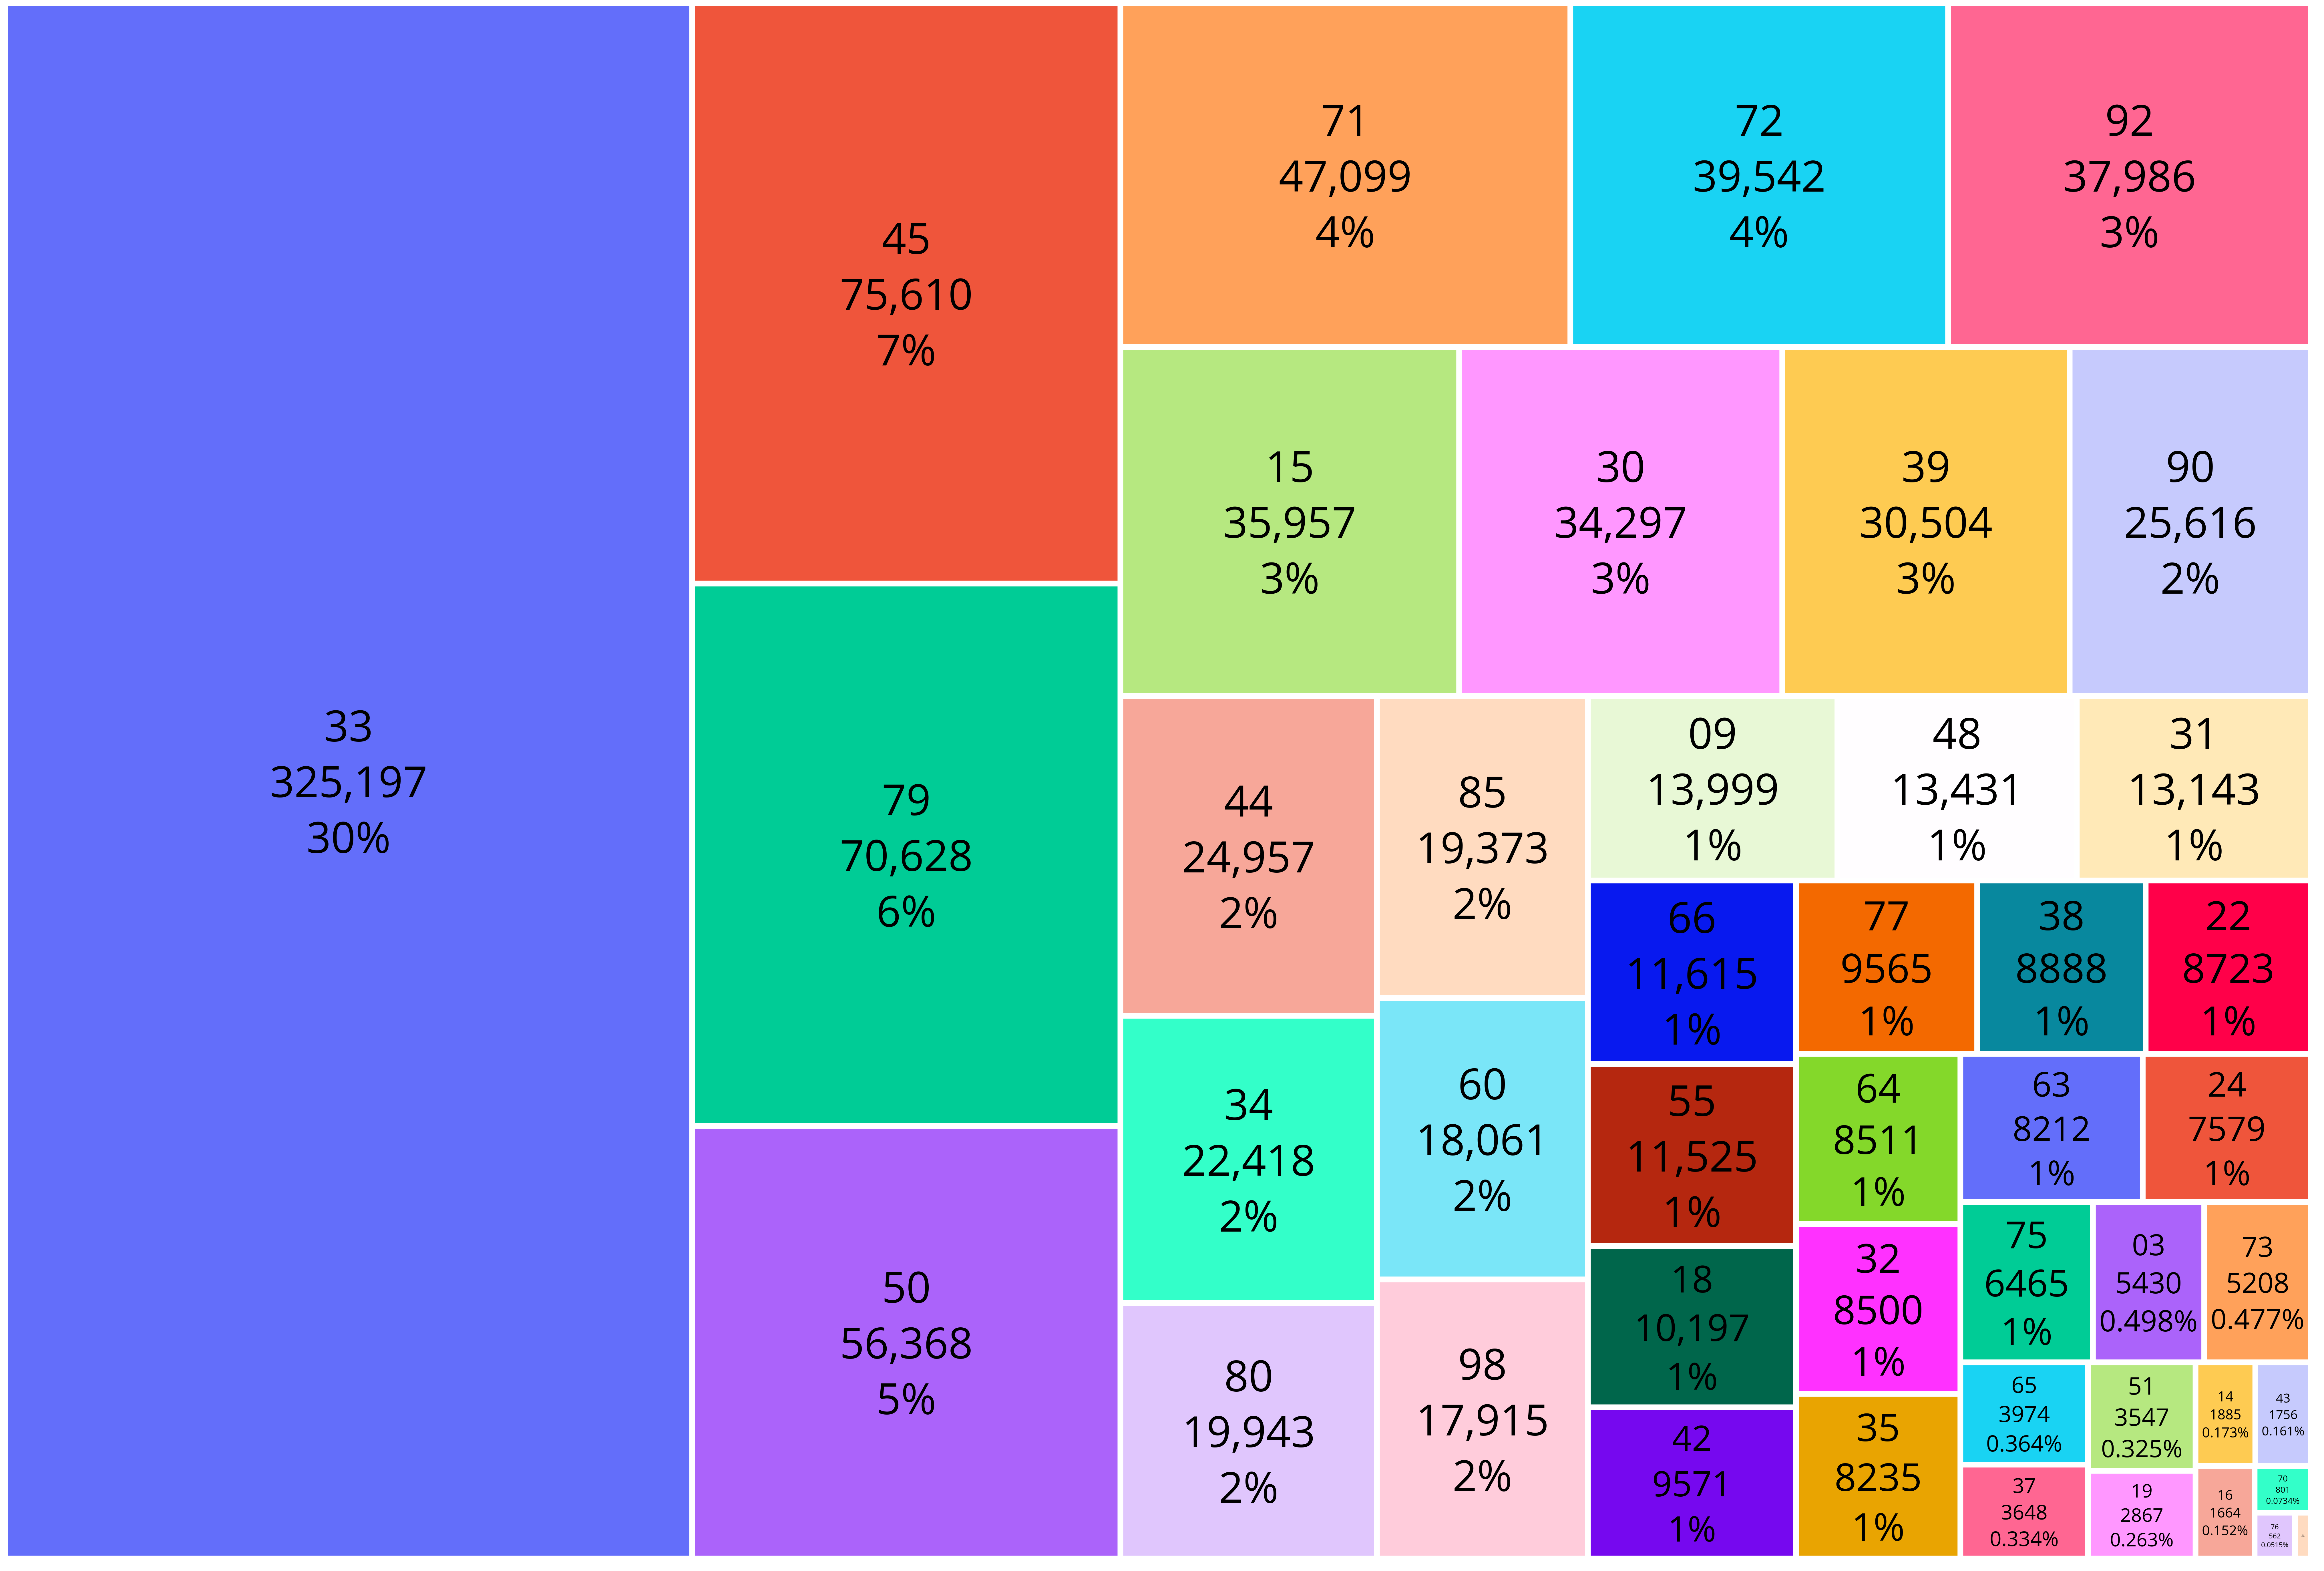
\includegraphics[width=\textwidth]{imagens/treemap_contratos.png}
	\caption{Distribuição do número de contratos públicos, por divisão do CPV.}
	\label{fig:cpvs}
\end{figure}
\vfill
\clearpage


\begin{wrapfigure}{R}{0.49\textwidth}
	\centering
	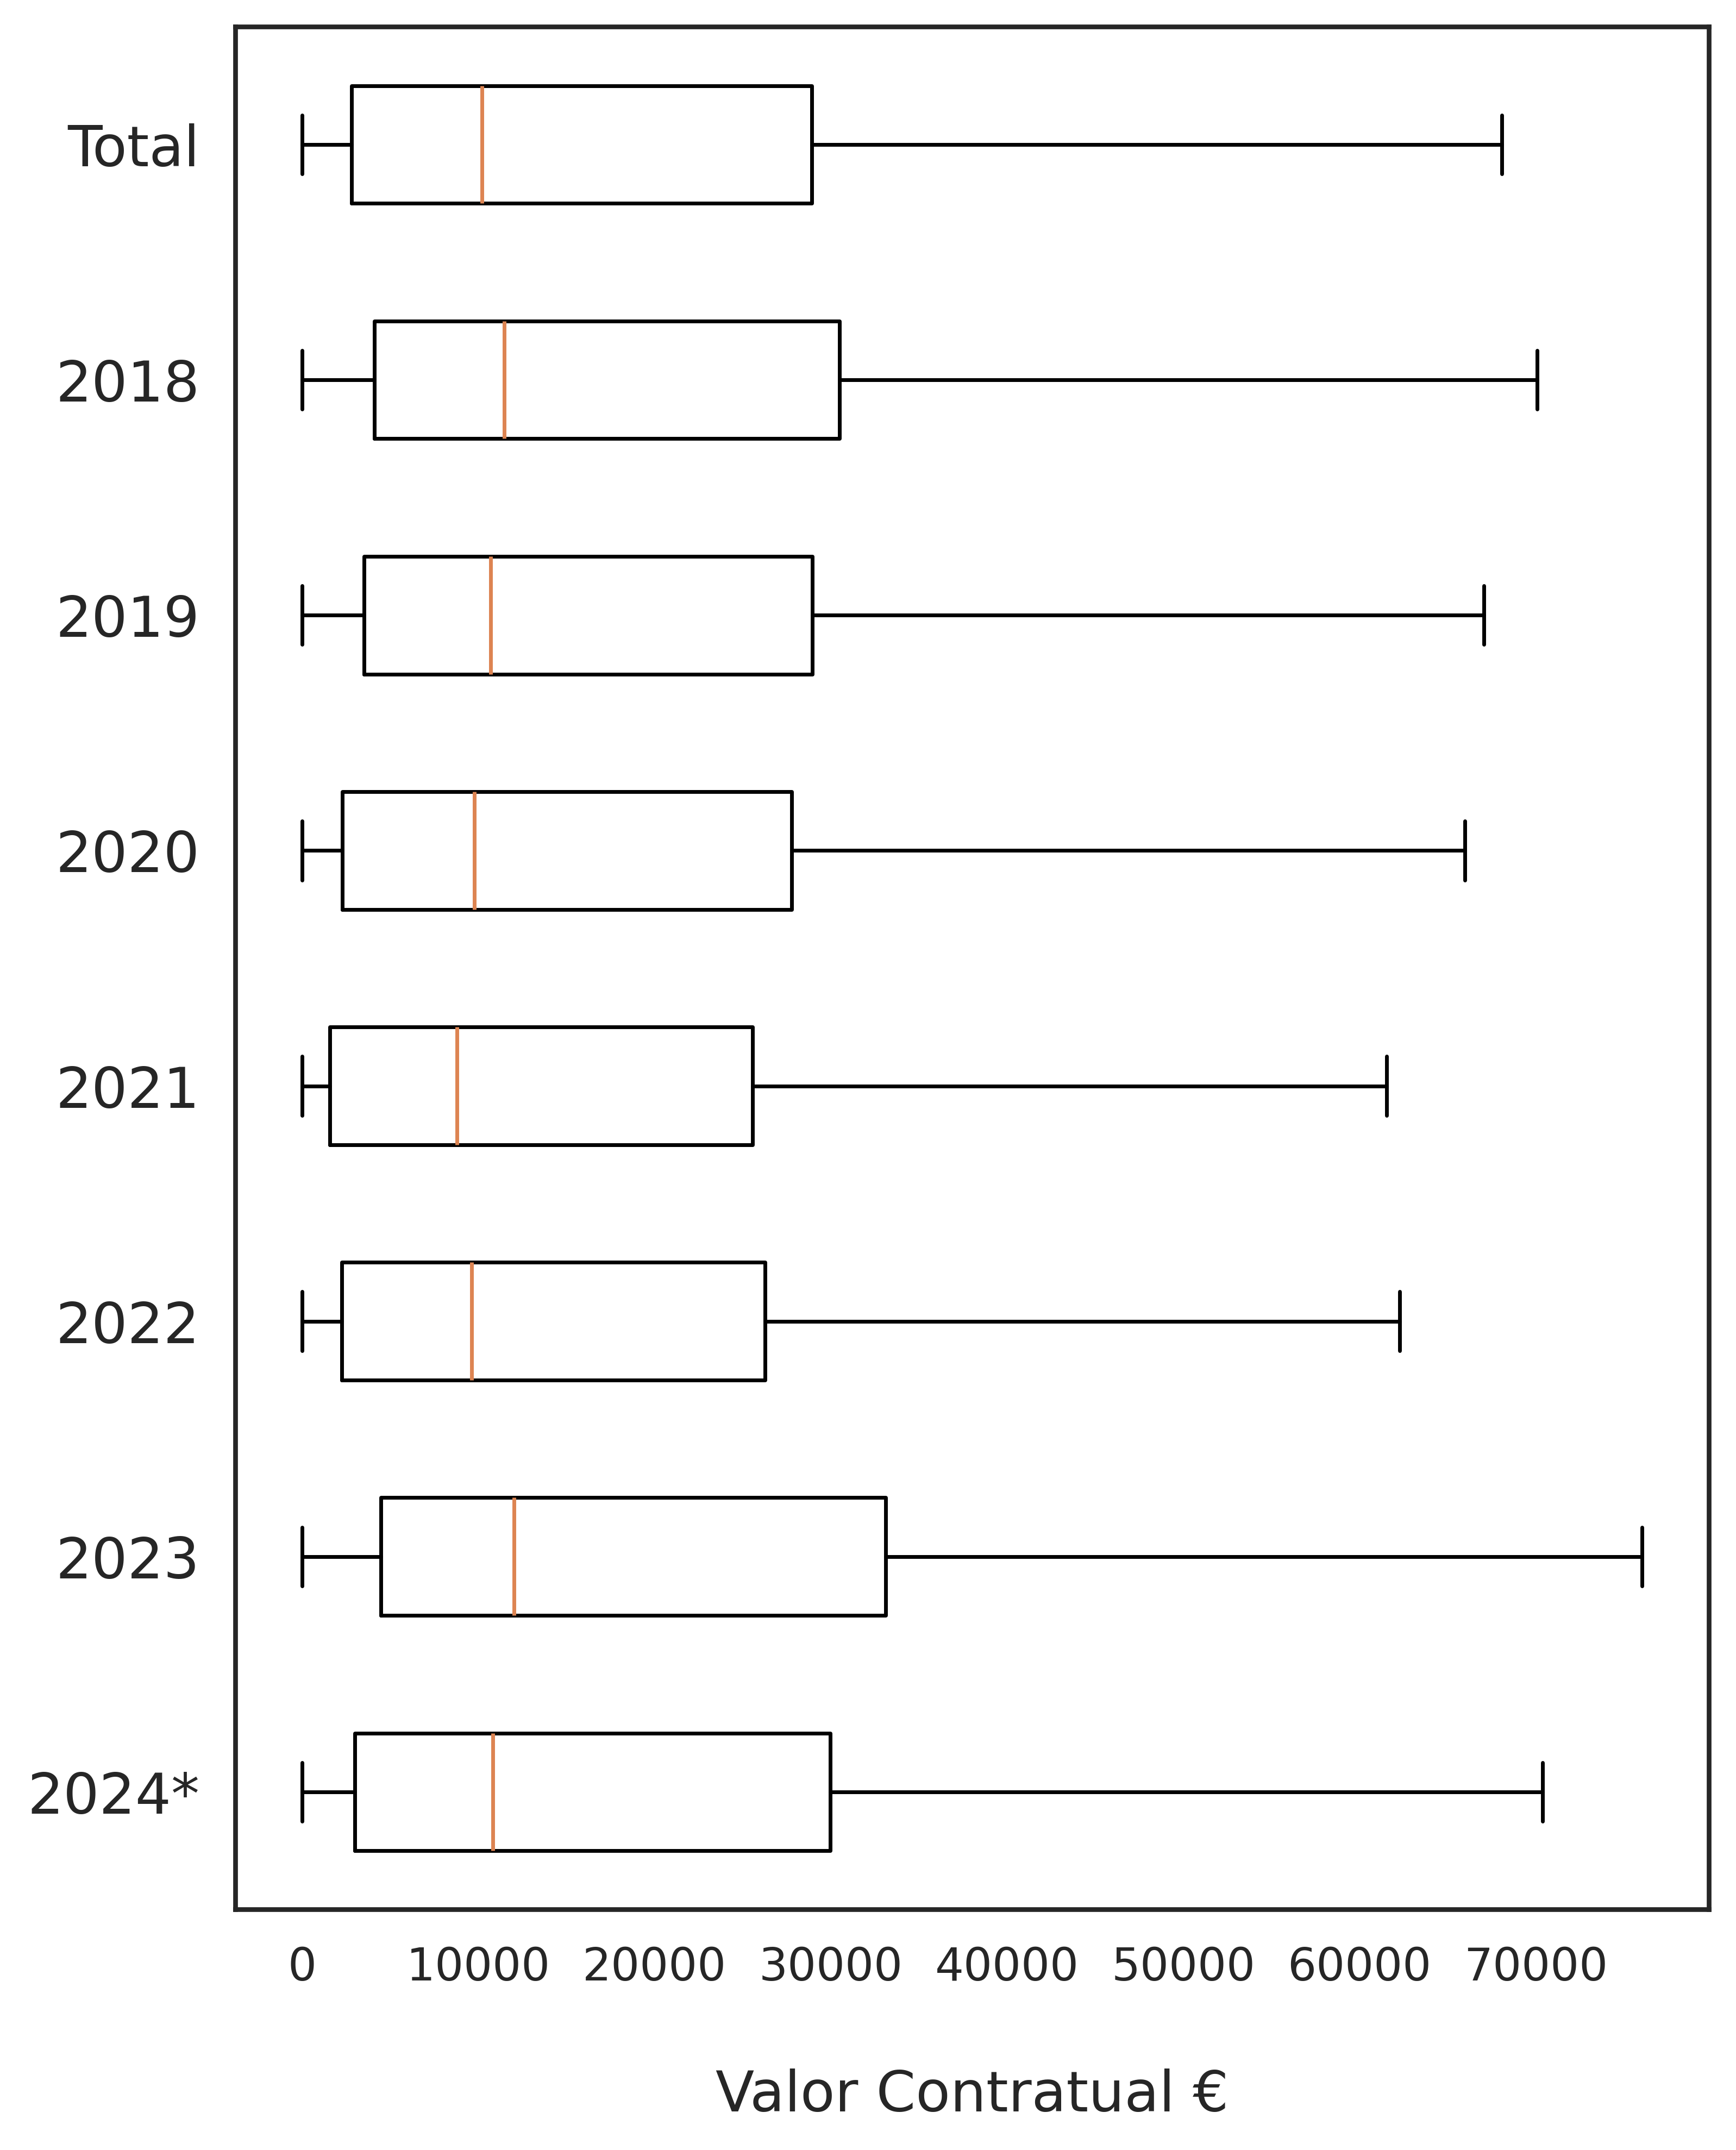
\includegraphics[width=0.49\textwidth]{imagens/precoscontr_stat.png}
	\caption{Boxplot dos preços contratuais para toda a tipologia de contratos desde 2018 até 2024}
	\label{fig:precotodos}
\end{wrapfigure}


Outra das variáveis com especial relevância e que foi considerada ao longo do projeto é o preço contratual. A Figura \ref{fig:precotodos} representa os \textit{boxplots} referentes aos preços contratuais para todos os contratos da base de dados, independentemente da tipologia de procedimento, por ano e durante o período de tempo considerado (de 2018 a 2024). É importante sublinhar que, tendo em conta que existem 2672 contratos cujo preço contratual é nulo, estes gráficos são meramente ilustrativos, correndo assim um desfasamento entre a informação apresentada e os valores reais. Pode-se observar que os valores dos 1º, 2º e 3º quartis tomam, sensivelmente, valores próximos para todos os anos. A distância interquartil é, aproximadamente, a mesma para os anos considerados e a distribuição dos valores é claramente assimétrica à direita. Porém, tendo em conta que neste cálculo são consideradas todas as tipologias de contratos e todas as divisões de CPV, esta informação não é conclusiva. Evidentemente, os valores adjudicados aos contratos referentes à construção civil (45) são mais expressivos que os referentes a serviços recreativos, culturais e desportivos (92). Por sua vez, tal como foi apresentado no capítulo anterior, existem valores contratuais máximos permitidos mediante a tipologia de contrato. Desta forma, é natural que exista um elevado número de \textit{outliers}, não representados na Figura \ref{fig:precotodos}. \\
Ao longo deste estágio foram apenas consideradas duas tipologias de contratos: Ajustes Diretos em Regime Geral e Concursos Públicos. Assim, é oportuno incluir alguma descrição estatística destes dois casos. Foram construídos  \textit{boxplots} como representações gráficas relativas ao número de contratos e respetivo preço contratual total, por ano. Os resultados encontram-se nas Figuras \ref{fig:precocps}, \ref{fig:precocps1} e \ref{fig:precocps2}, para concursos públicos e nas Figuras \ref{fig:precoad}, \ref{fig:precoad1} e \ref{fig:precoad2}, para ajustes diretos em regime geral. 

Deste modo, possível observar que os valores contratuais dos concursos públicos, tal como observado na Figura \ref{fig:precocps}, são substancialmente superiores aos dos ajustes diretos, tal como ilustrado na Figura \ref{fig:precoad}. Apesar do número de contratos celebrados por ano para concursos públicos, tal como indicado na Figura \ref{fig:precocps1}, ser sempre inferior ao de ajustes diretos - Figura \ref{fig:precoad1} -, o valor adjudicado, por ano, foi sempre superior ao dos ajustes diretos. Deste modo, pode concluir-se que os valores contratuais de concursos públicos tem, necessariamente, de ser superiores. Em ambos os casos, as distribuições dos valores contratuais são assimétricas. 

No caso dos concursos públicos, 23\% dos contratos celebrados referem-se à aquisição de equipamento médico e 17\% a obras de contrução civil (ver Figura \ref{fig:cpcpv}), sendo que cerca de 25\% são celebrados no distrito de Lisboa, 10\% no Porto e 11\% em distritos indeterminados (ver Figura \ref{fig:cploc}). Relativamente a ajustes diretos, existe uma predominância de contratos referentes à aquisição de equipamento médico, totalizando 28\% dos contratos celebrados (ver Figura \ref{fig:adcpv}), com maior destaque para os distritos de Lisboa, com 23\% e Porto, com 17\%  (ver Figura \ref{fig:adloc}).

\vfill

\begin{figure}[H]
	\centering
	\begin{minipage}{0.31\linewidth}
		%\centering  % redundant
		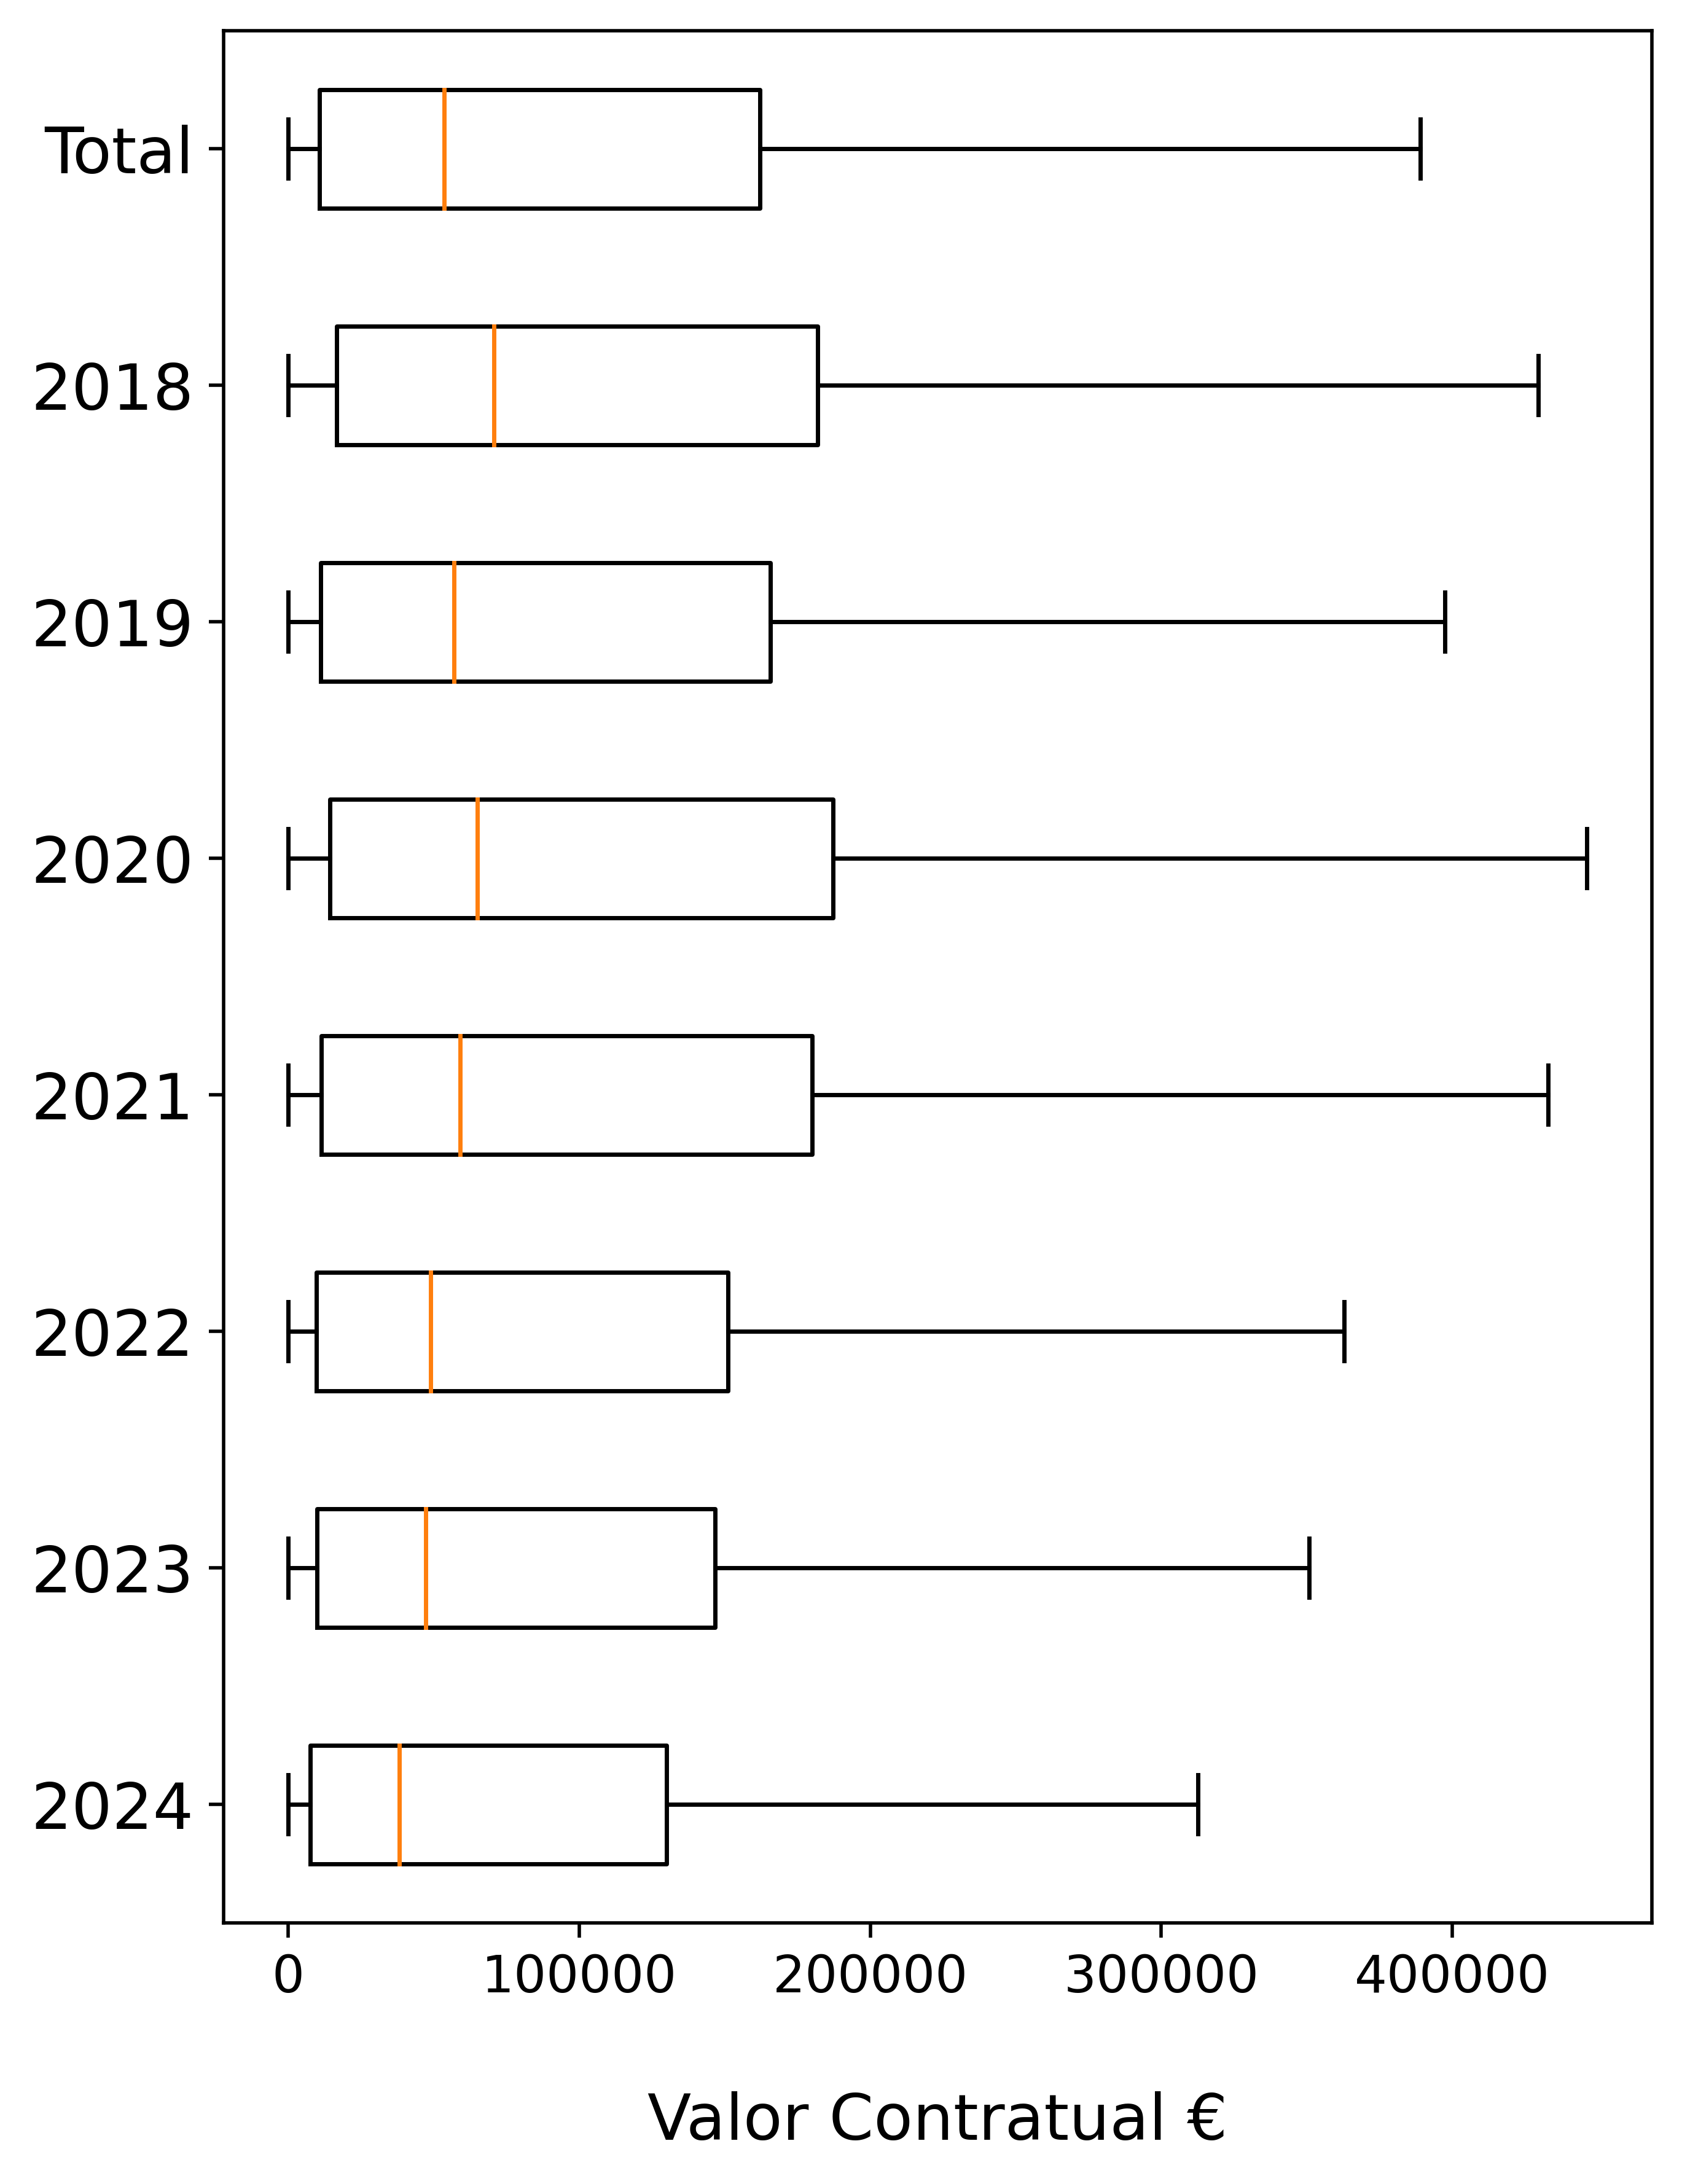
\includegraphics[width=\textwidth]{imagens/concpub_stat.png}
		\caption{Boxplot dos preços contratuais para concursos públicos entre 2018 até 2024.}
		\label{fig:precocps}
	\end{minipage}
	\hfill
	\begin{minipage}{.31\linewidth}
		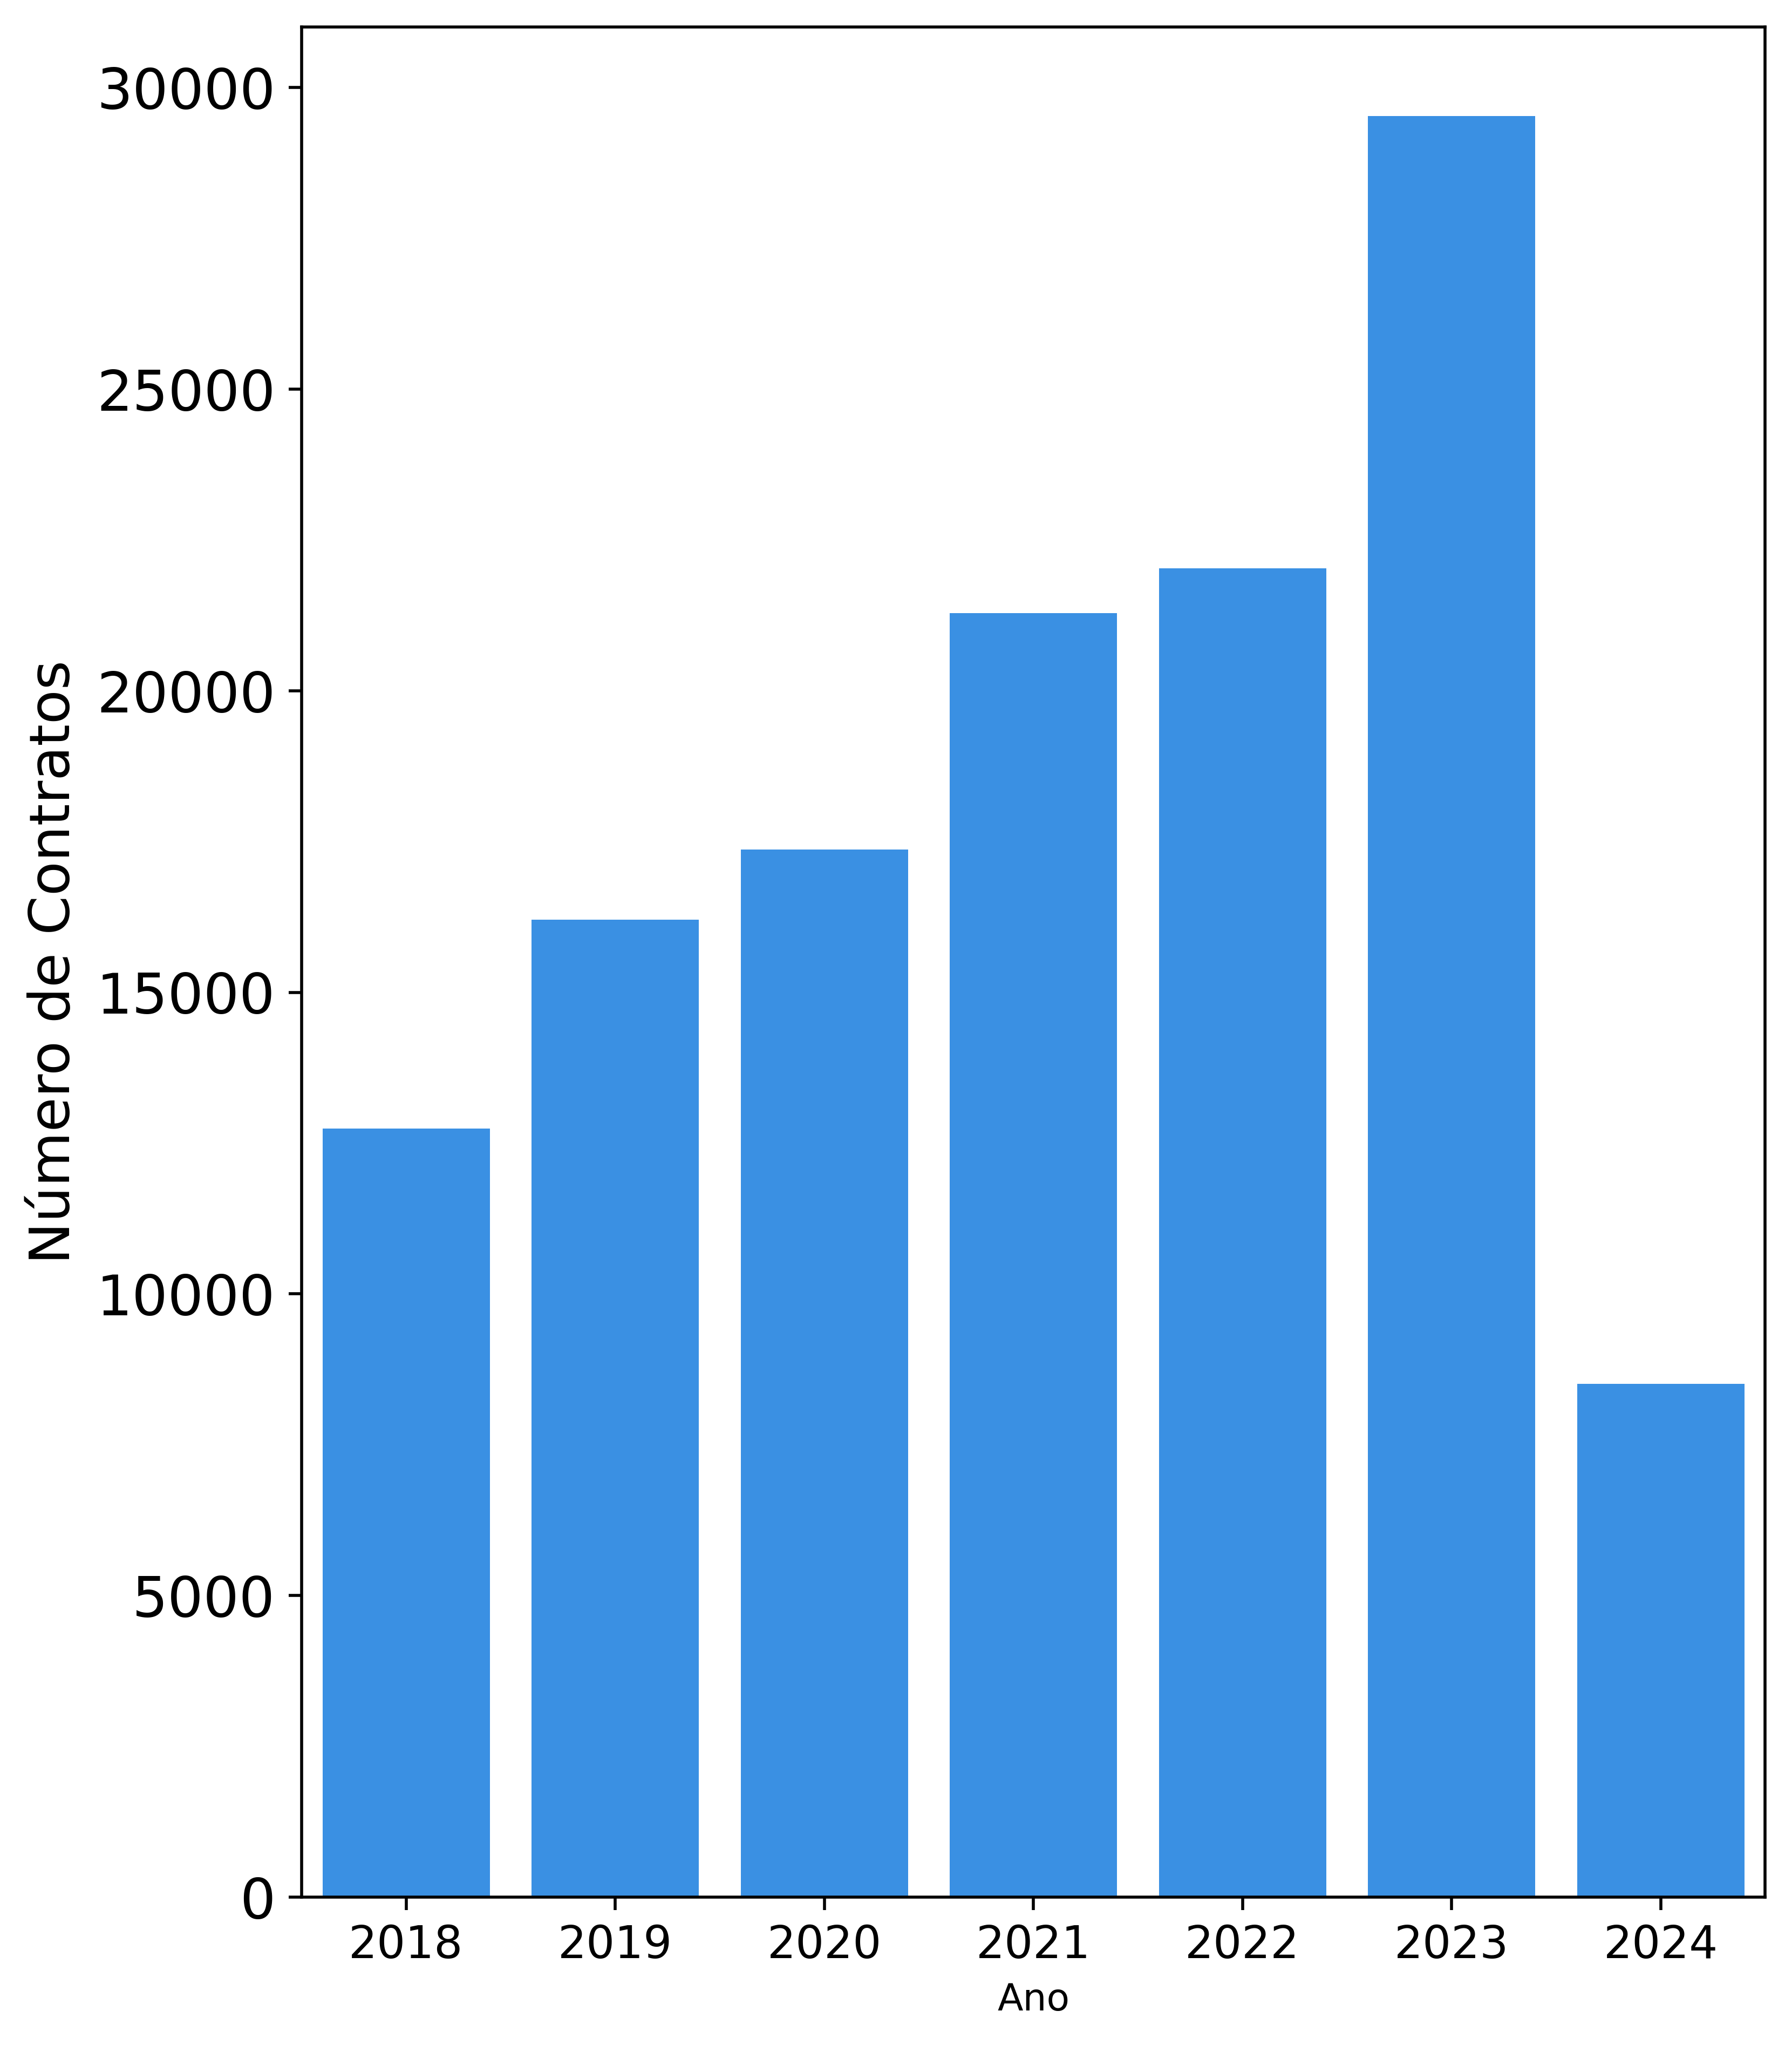
\includegraphics[width=\linewidth]{imagens/cpub_nrcontr.png}
		\caption{Número de concursos públicos celebrados, entre 2018 e 2024.}
		\label{fig:precocps1}
	\end{minipage}
	\hfill
	\begin{minipage}{.31\linewidth}
		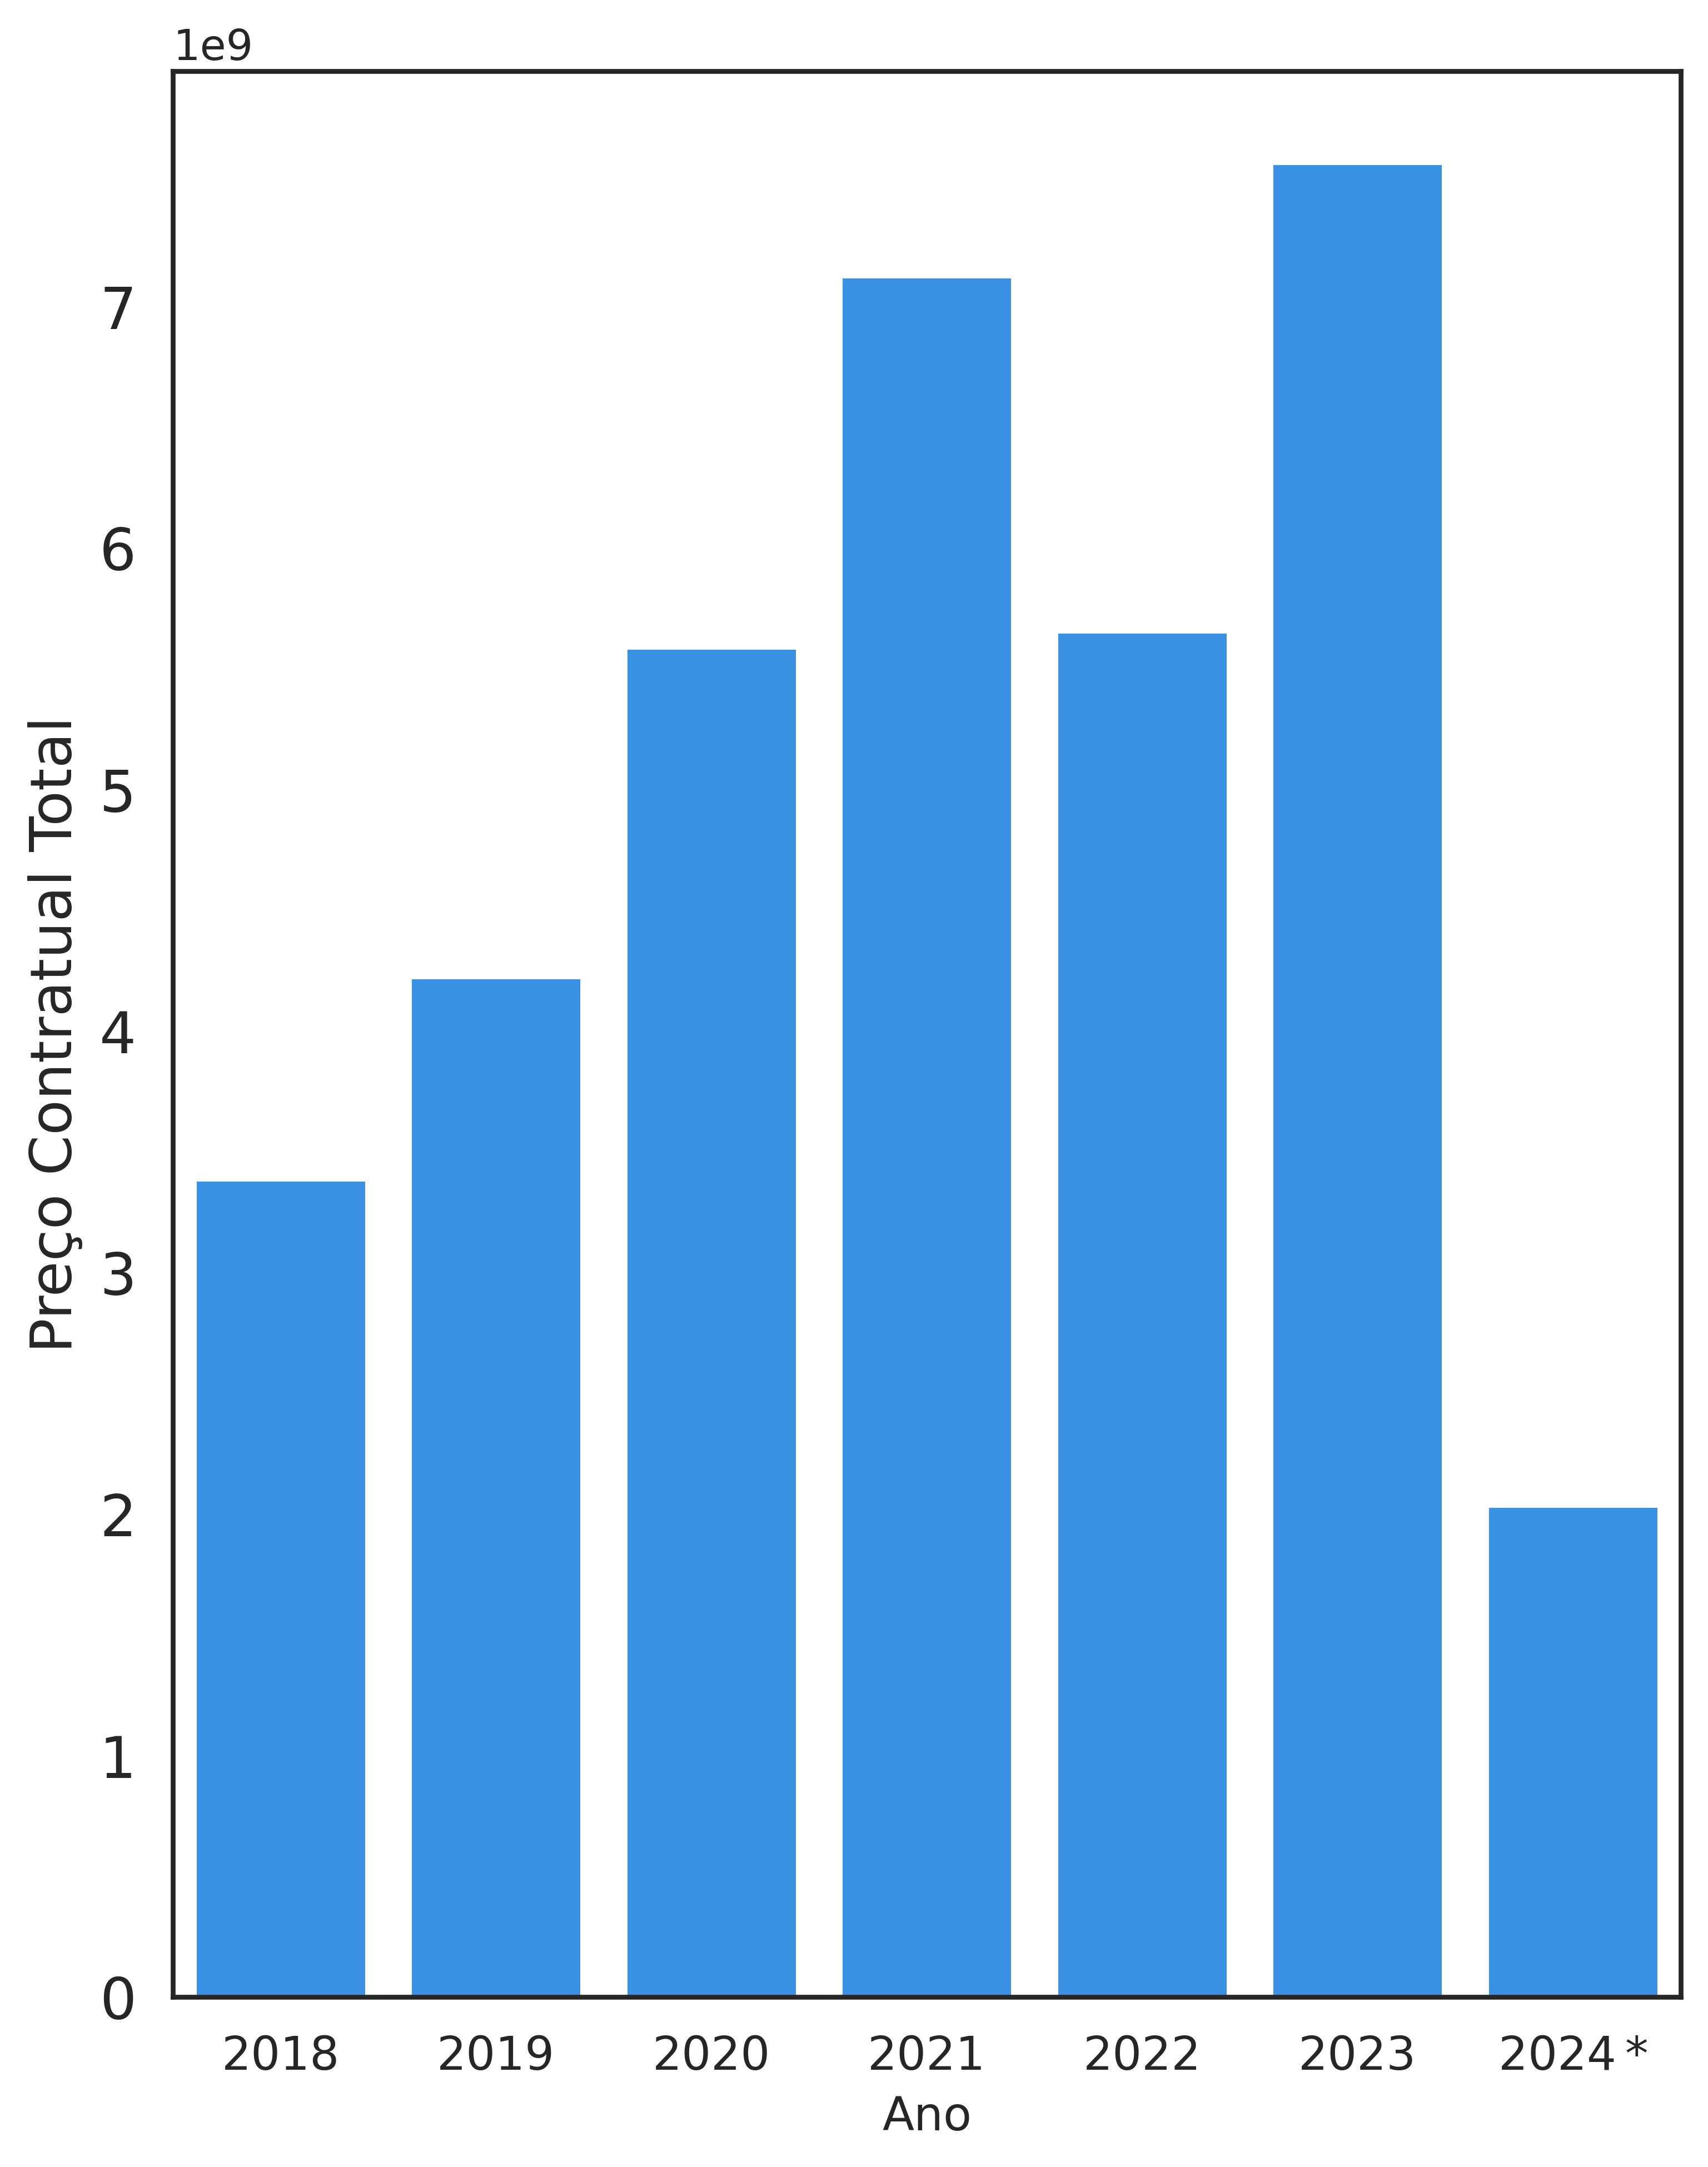
\includegraphics[width=\linewidth]{imagens/cpub_price.png}
		\caption{Preço contratual total, entre 2018 e 2024, para concursos públicos.}
		\label{fig:precocps2}
	\end{minipage}
\end{figure}

\vfill

\begin{figure}[H]
	\centering
	\begin{minipage}{.31\linewidth}
		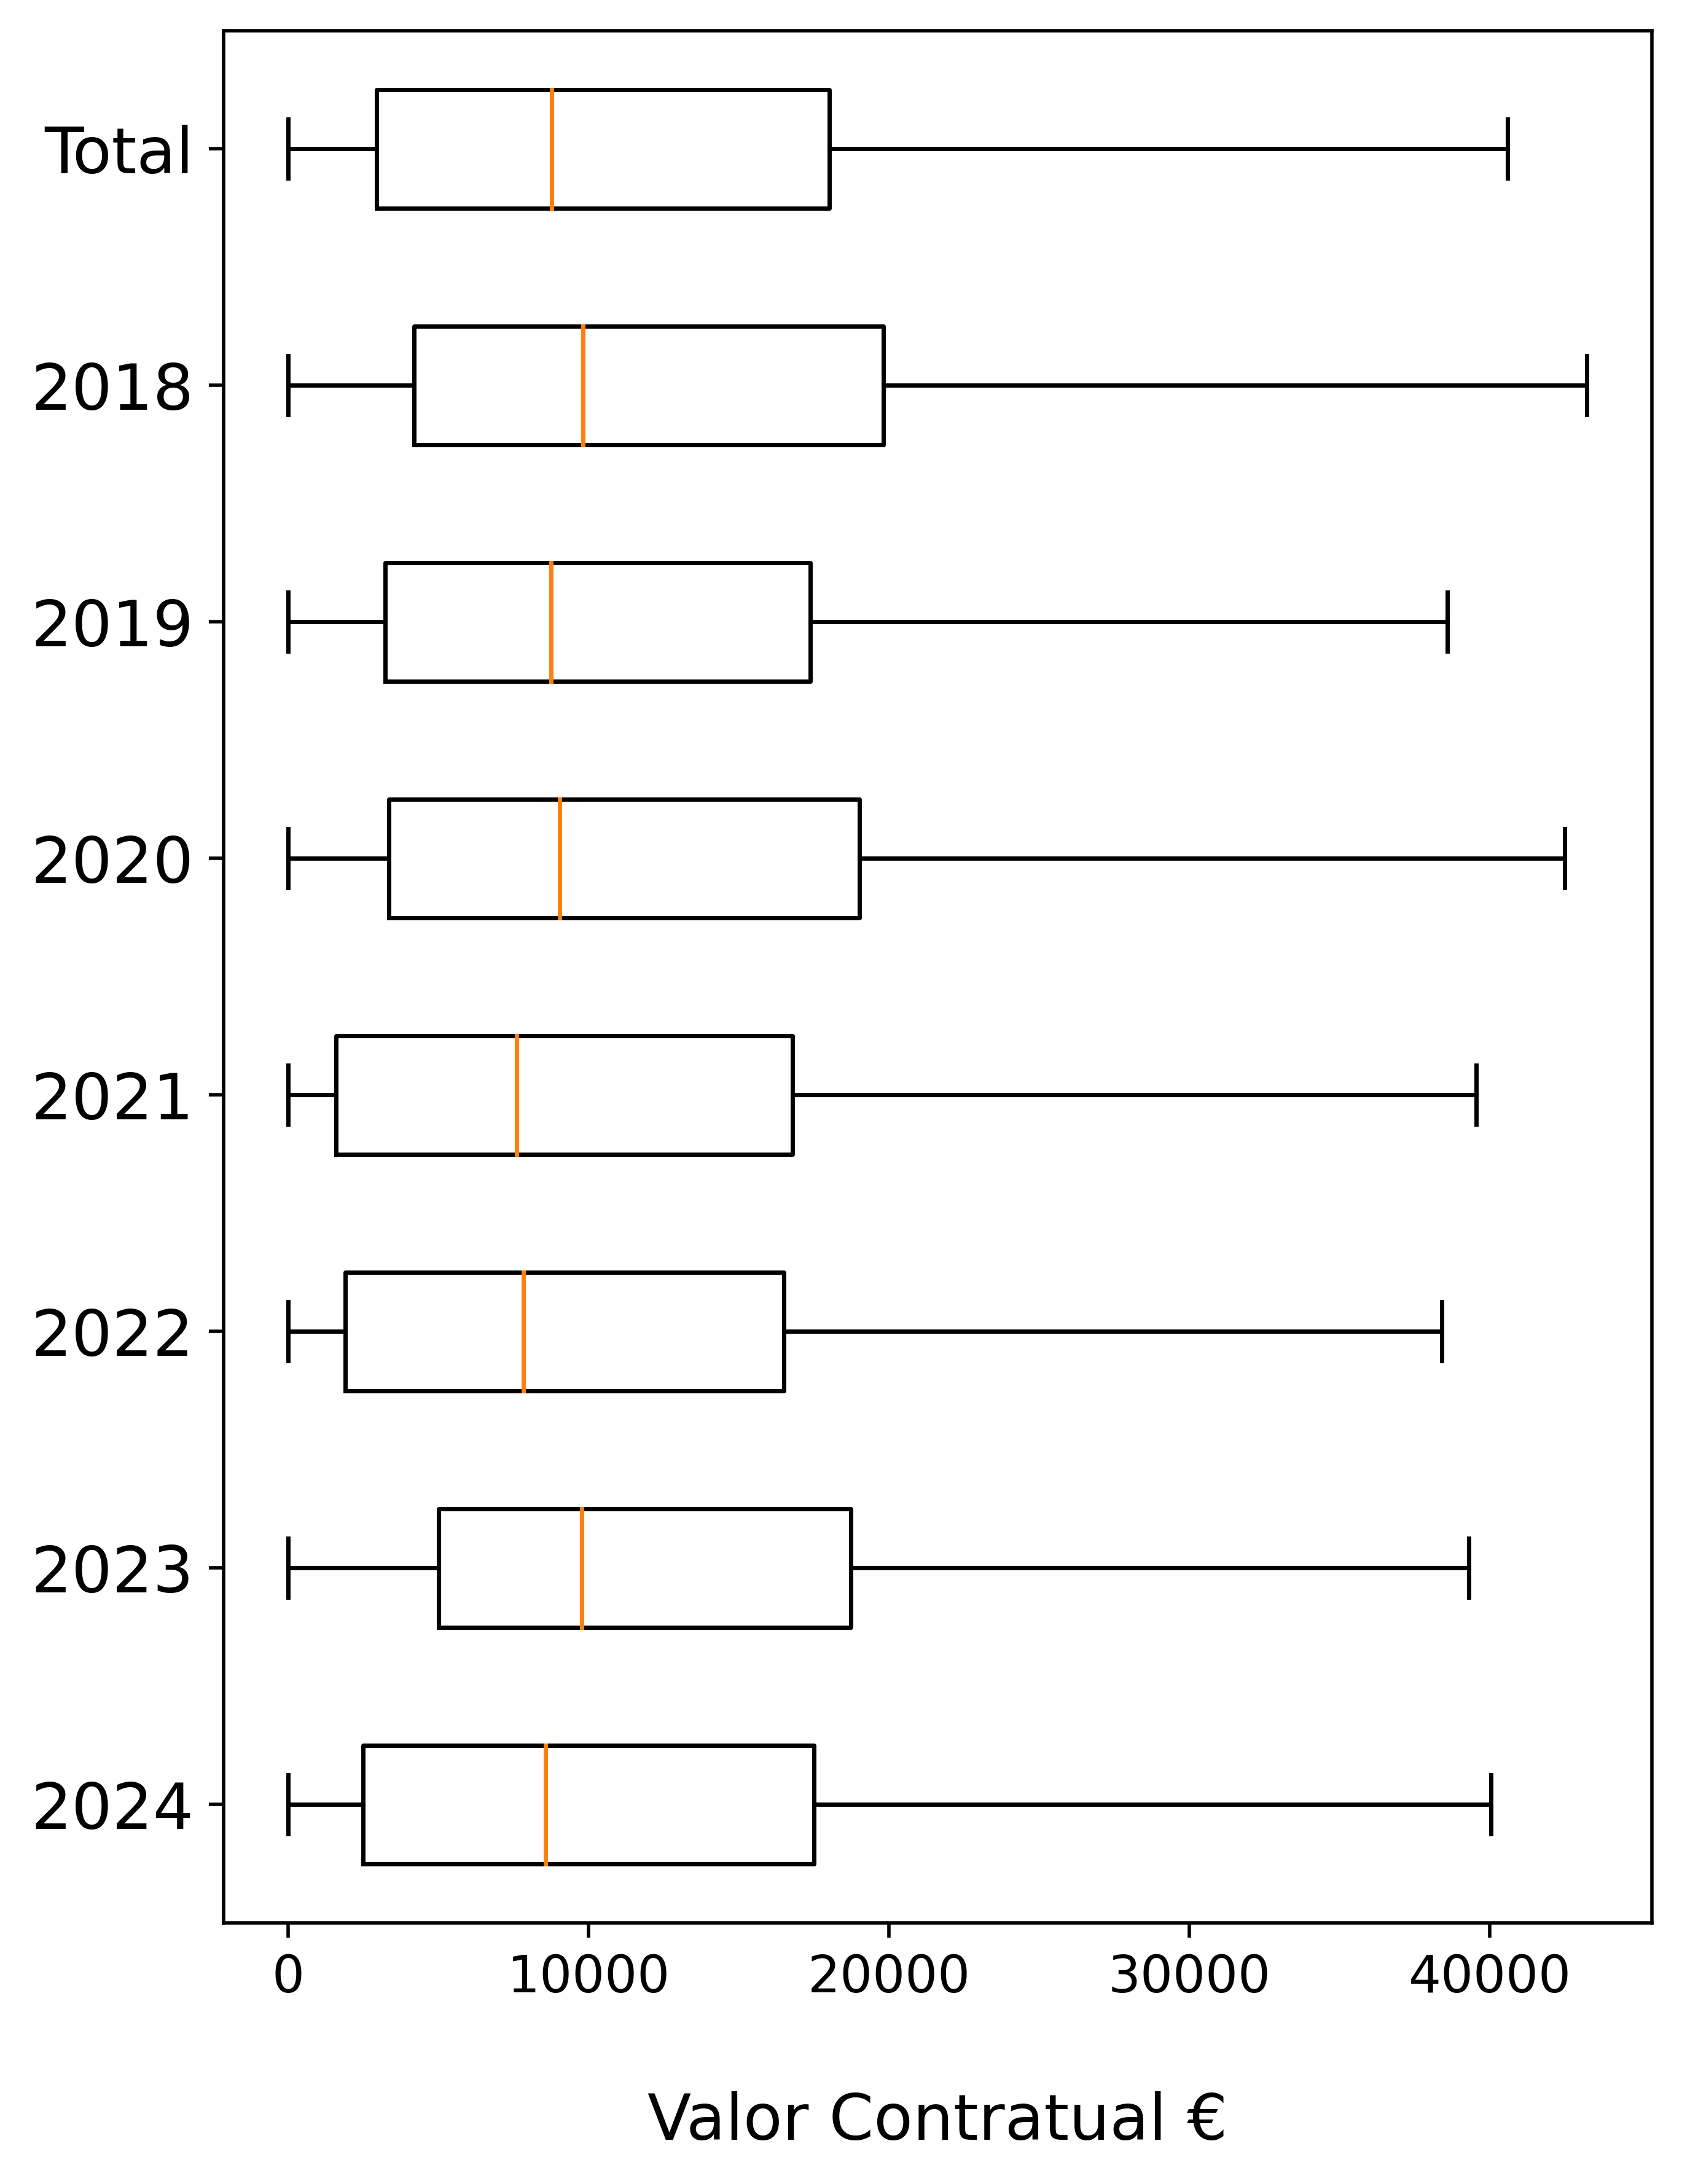
\includegraphics[width=\linewidth]{imagens/adir_stat.png}
		\caption{Boxplot dos preços contratuais de ajustes diretos celebrados, entre 2018 e 2024.}
		\label{fig:precoad}
	\end{minipage}
	\hfill
	\begin{minipage}{0.31\linewidth}
		%\centering  % redundant
		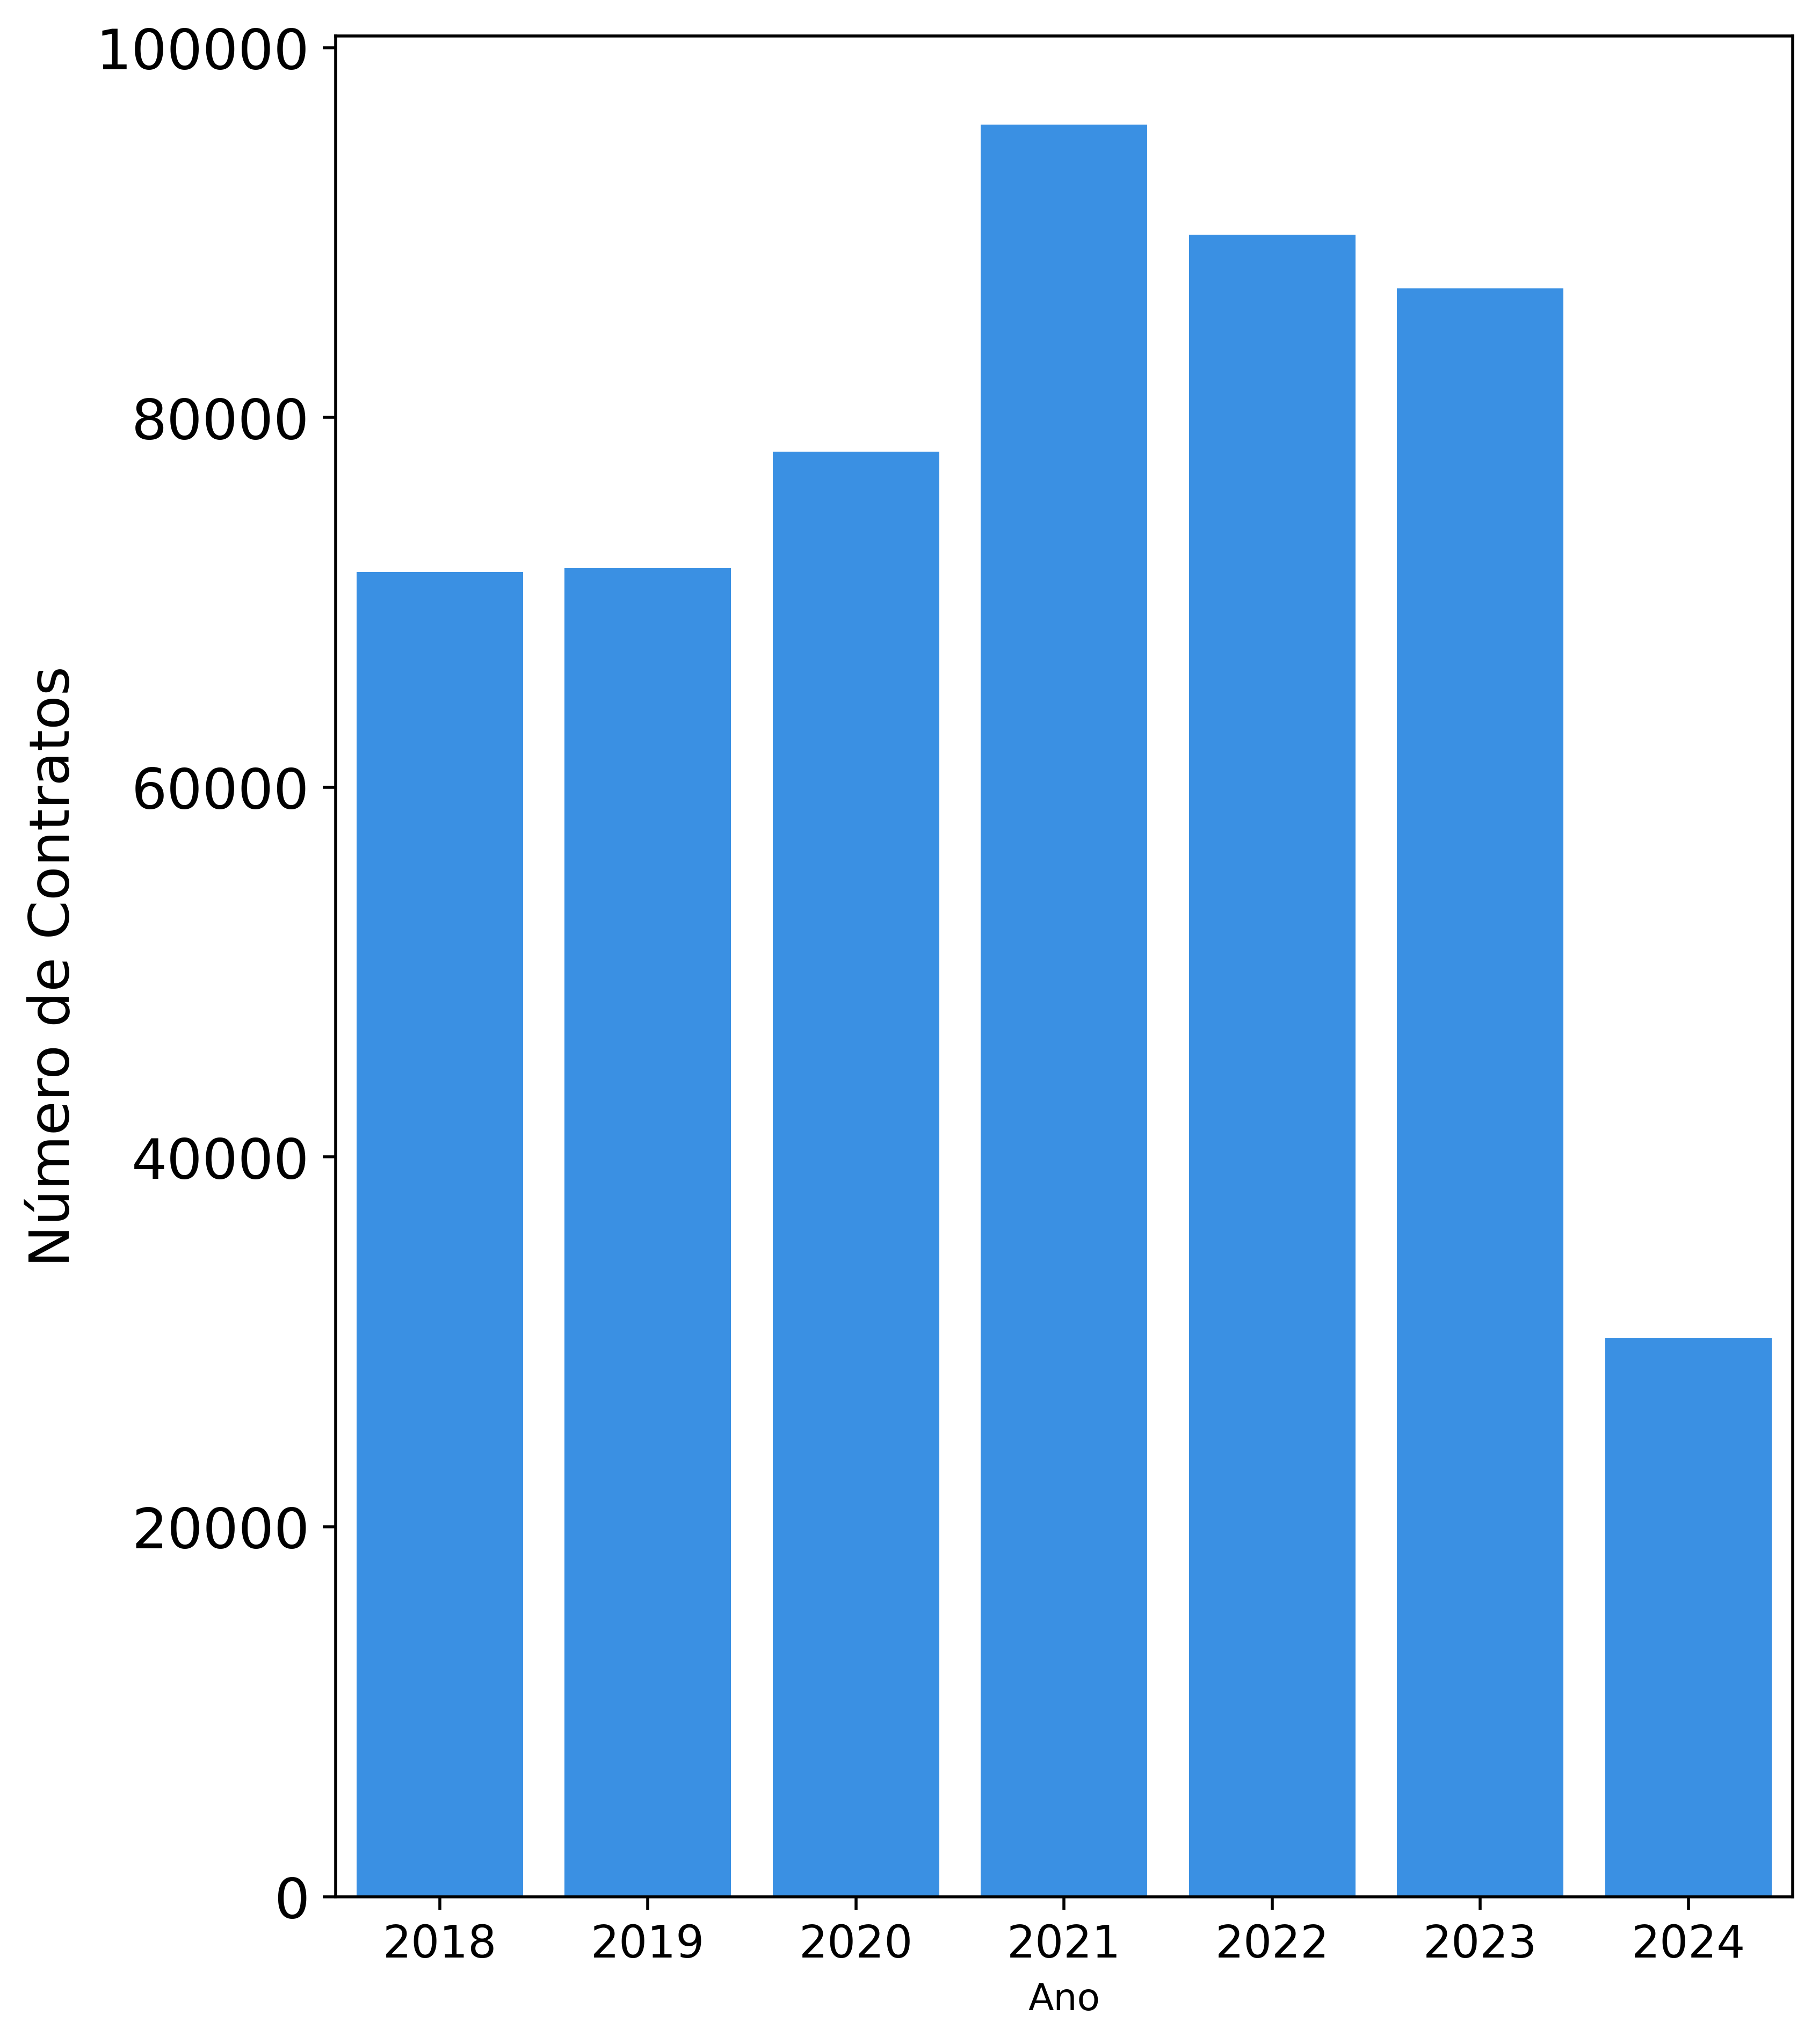
\includegraphics[width=\linewidth]{imagens/adir_nrcontr.png}
		\caption{Número de ajustes diretos celebrados, entre 2018 e 2024.}
		\label{fig:precoad1}
	\end{minipage}
	\hfill
	\begin{minipage}{.31\linewidth}
		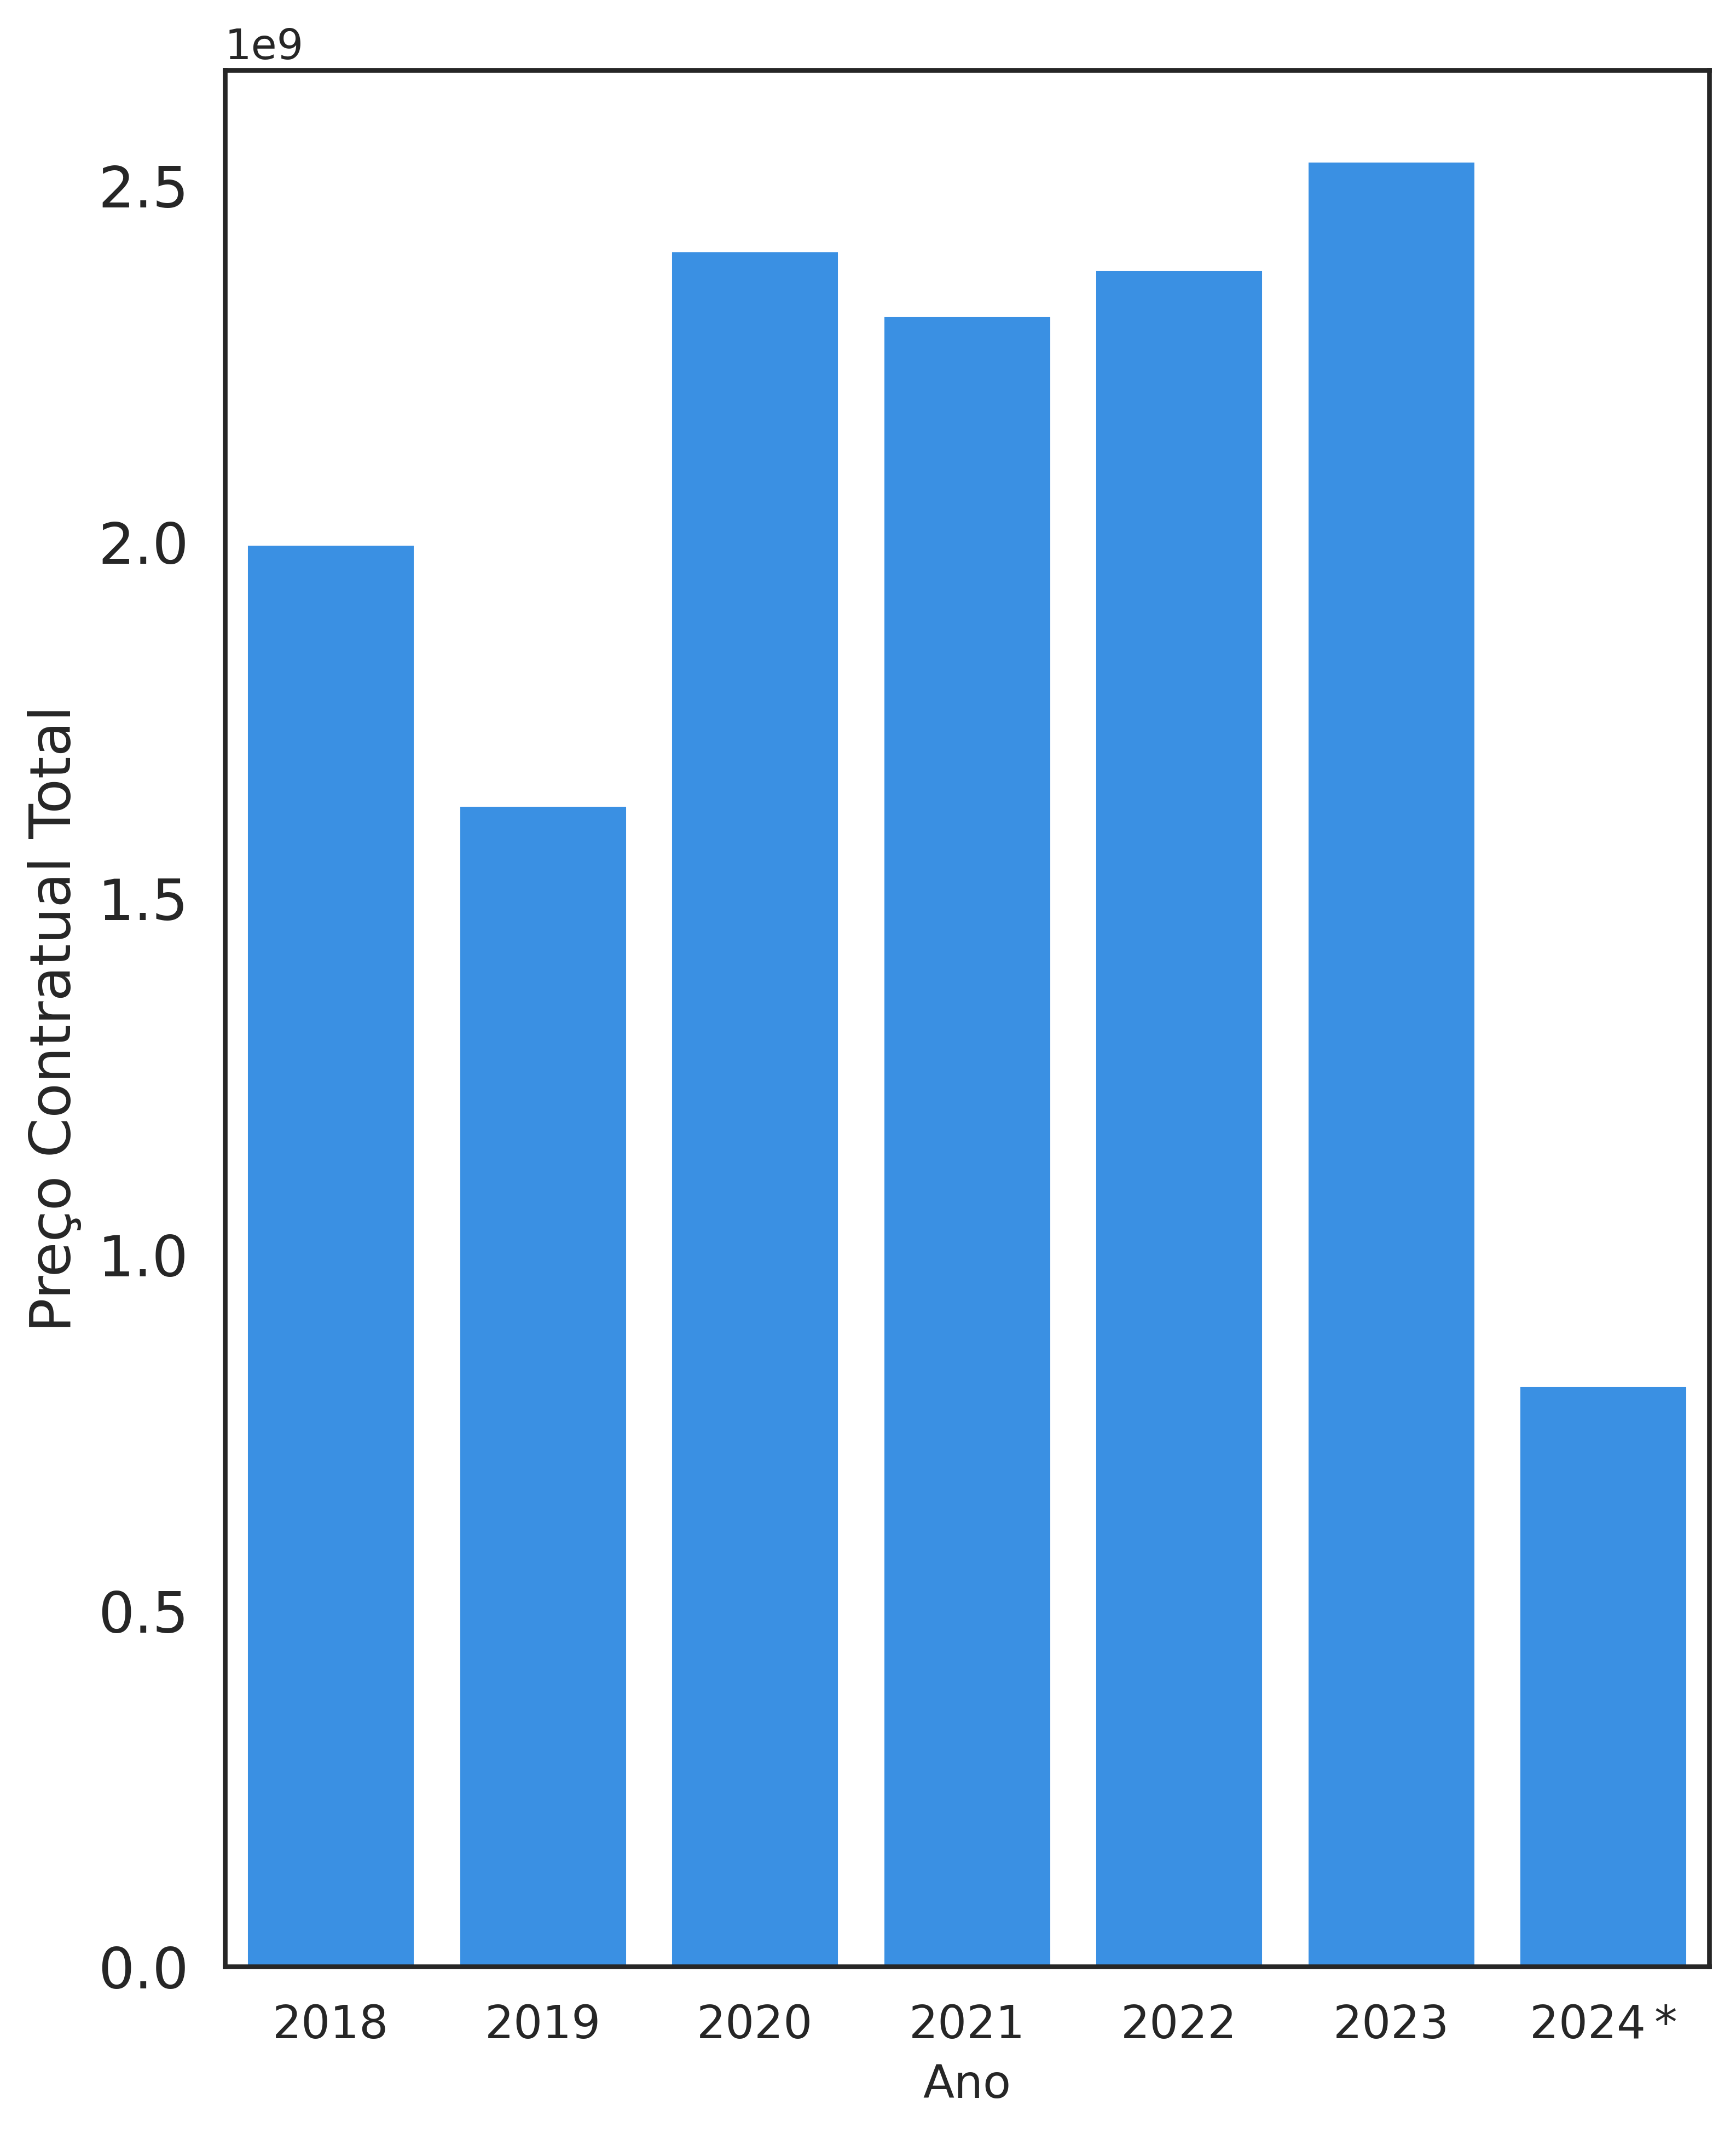
\includegraphics[width=\linewidth]{imagens/adir_price.png}
		\caption{Preço contratual total, entre 2018 e 2024, para ajustes diretos.}
		\label{fig:precoad2}
	\end{minipage}
\end{figure}


\clearpage
\begin{figure}[H]
	\centering
	
	\begin{minipage}[t]{0.49\textwidth}
		\centering
		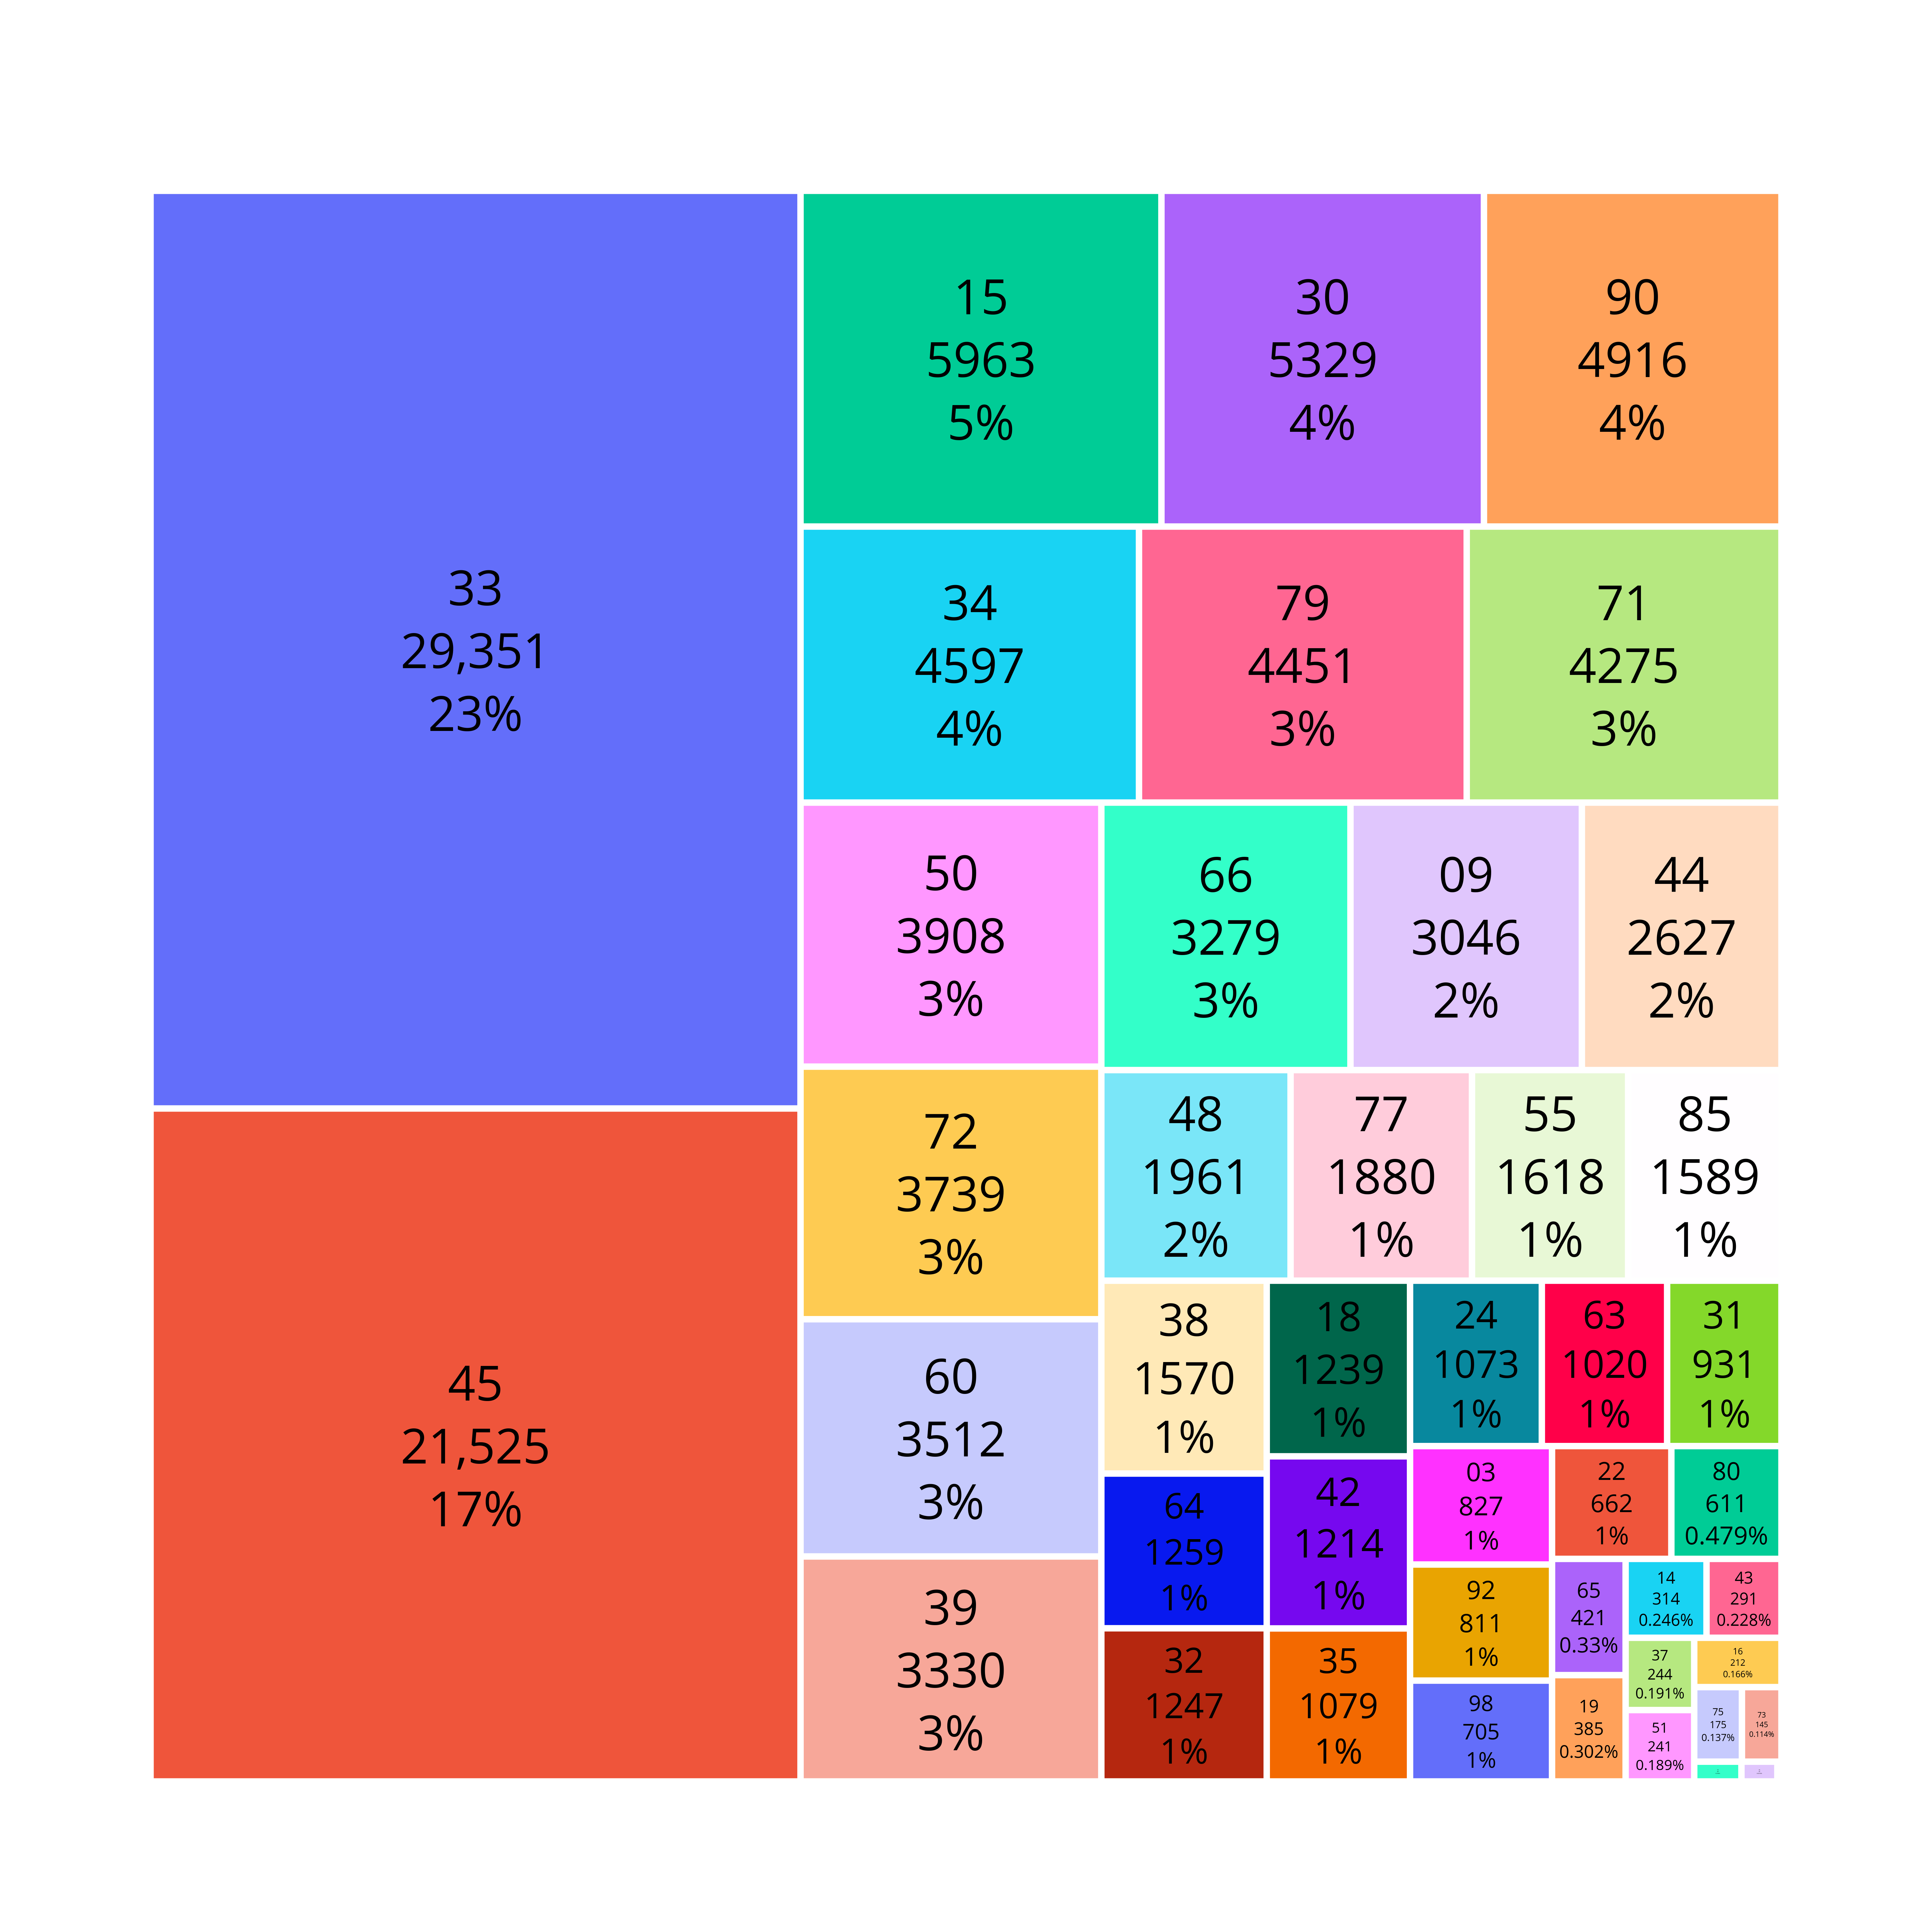
\includegraphics[width=\textwidth]{imagens/treemap_cpub.png}
		\caption{Distribuição do número de concursos públicos, por divisão de CPV.}
		\label{fig:cpcpv}
	\end{minipage}
	\hfill
	\begin{minipage}[t]{0.49\textwidth}
		\centering
		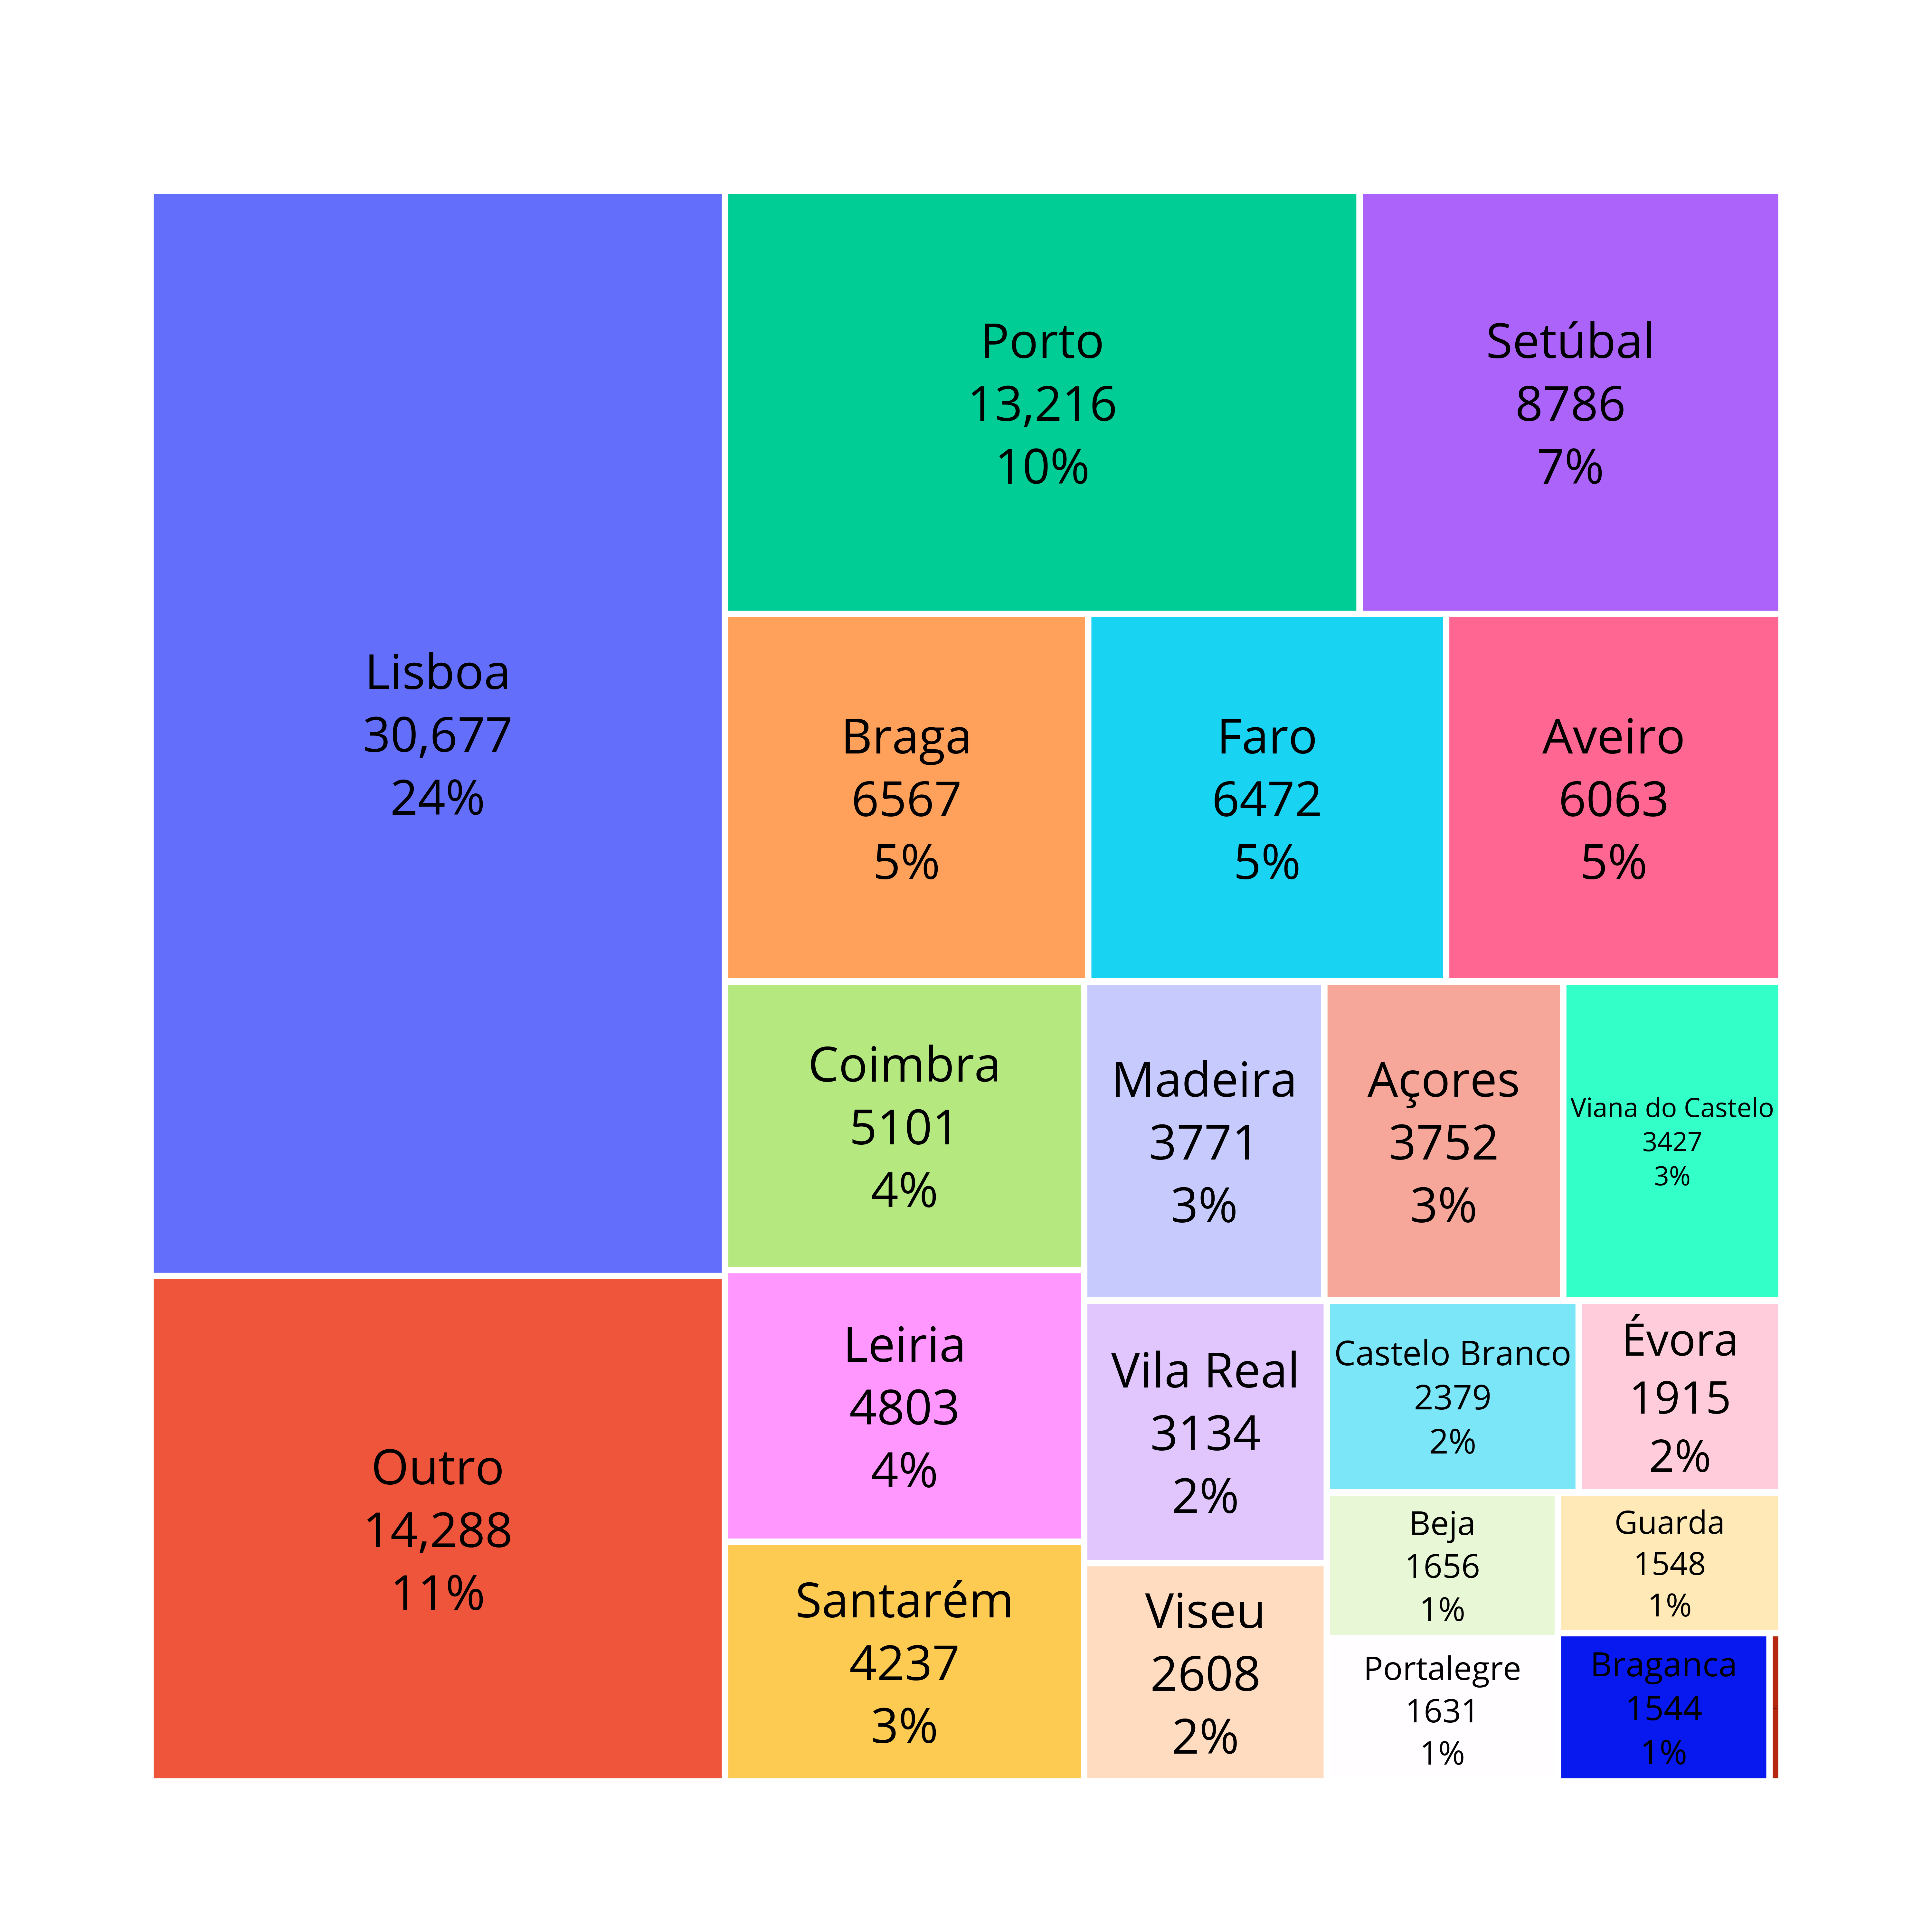
\includegraphics[width=\textwidth]{imagens/treemap_cpub_distritos.png}
		\caption{Distribuição do número de concursos públicos, por distrito.}
		\label{fig:cploc}
	\end{minipage}
	
	\vspace{1em}
	
	\begin{minipage}[t]{0.49\textwidth}
		\centering
		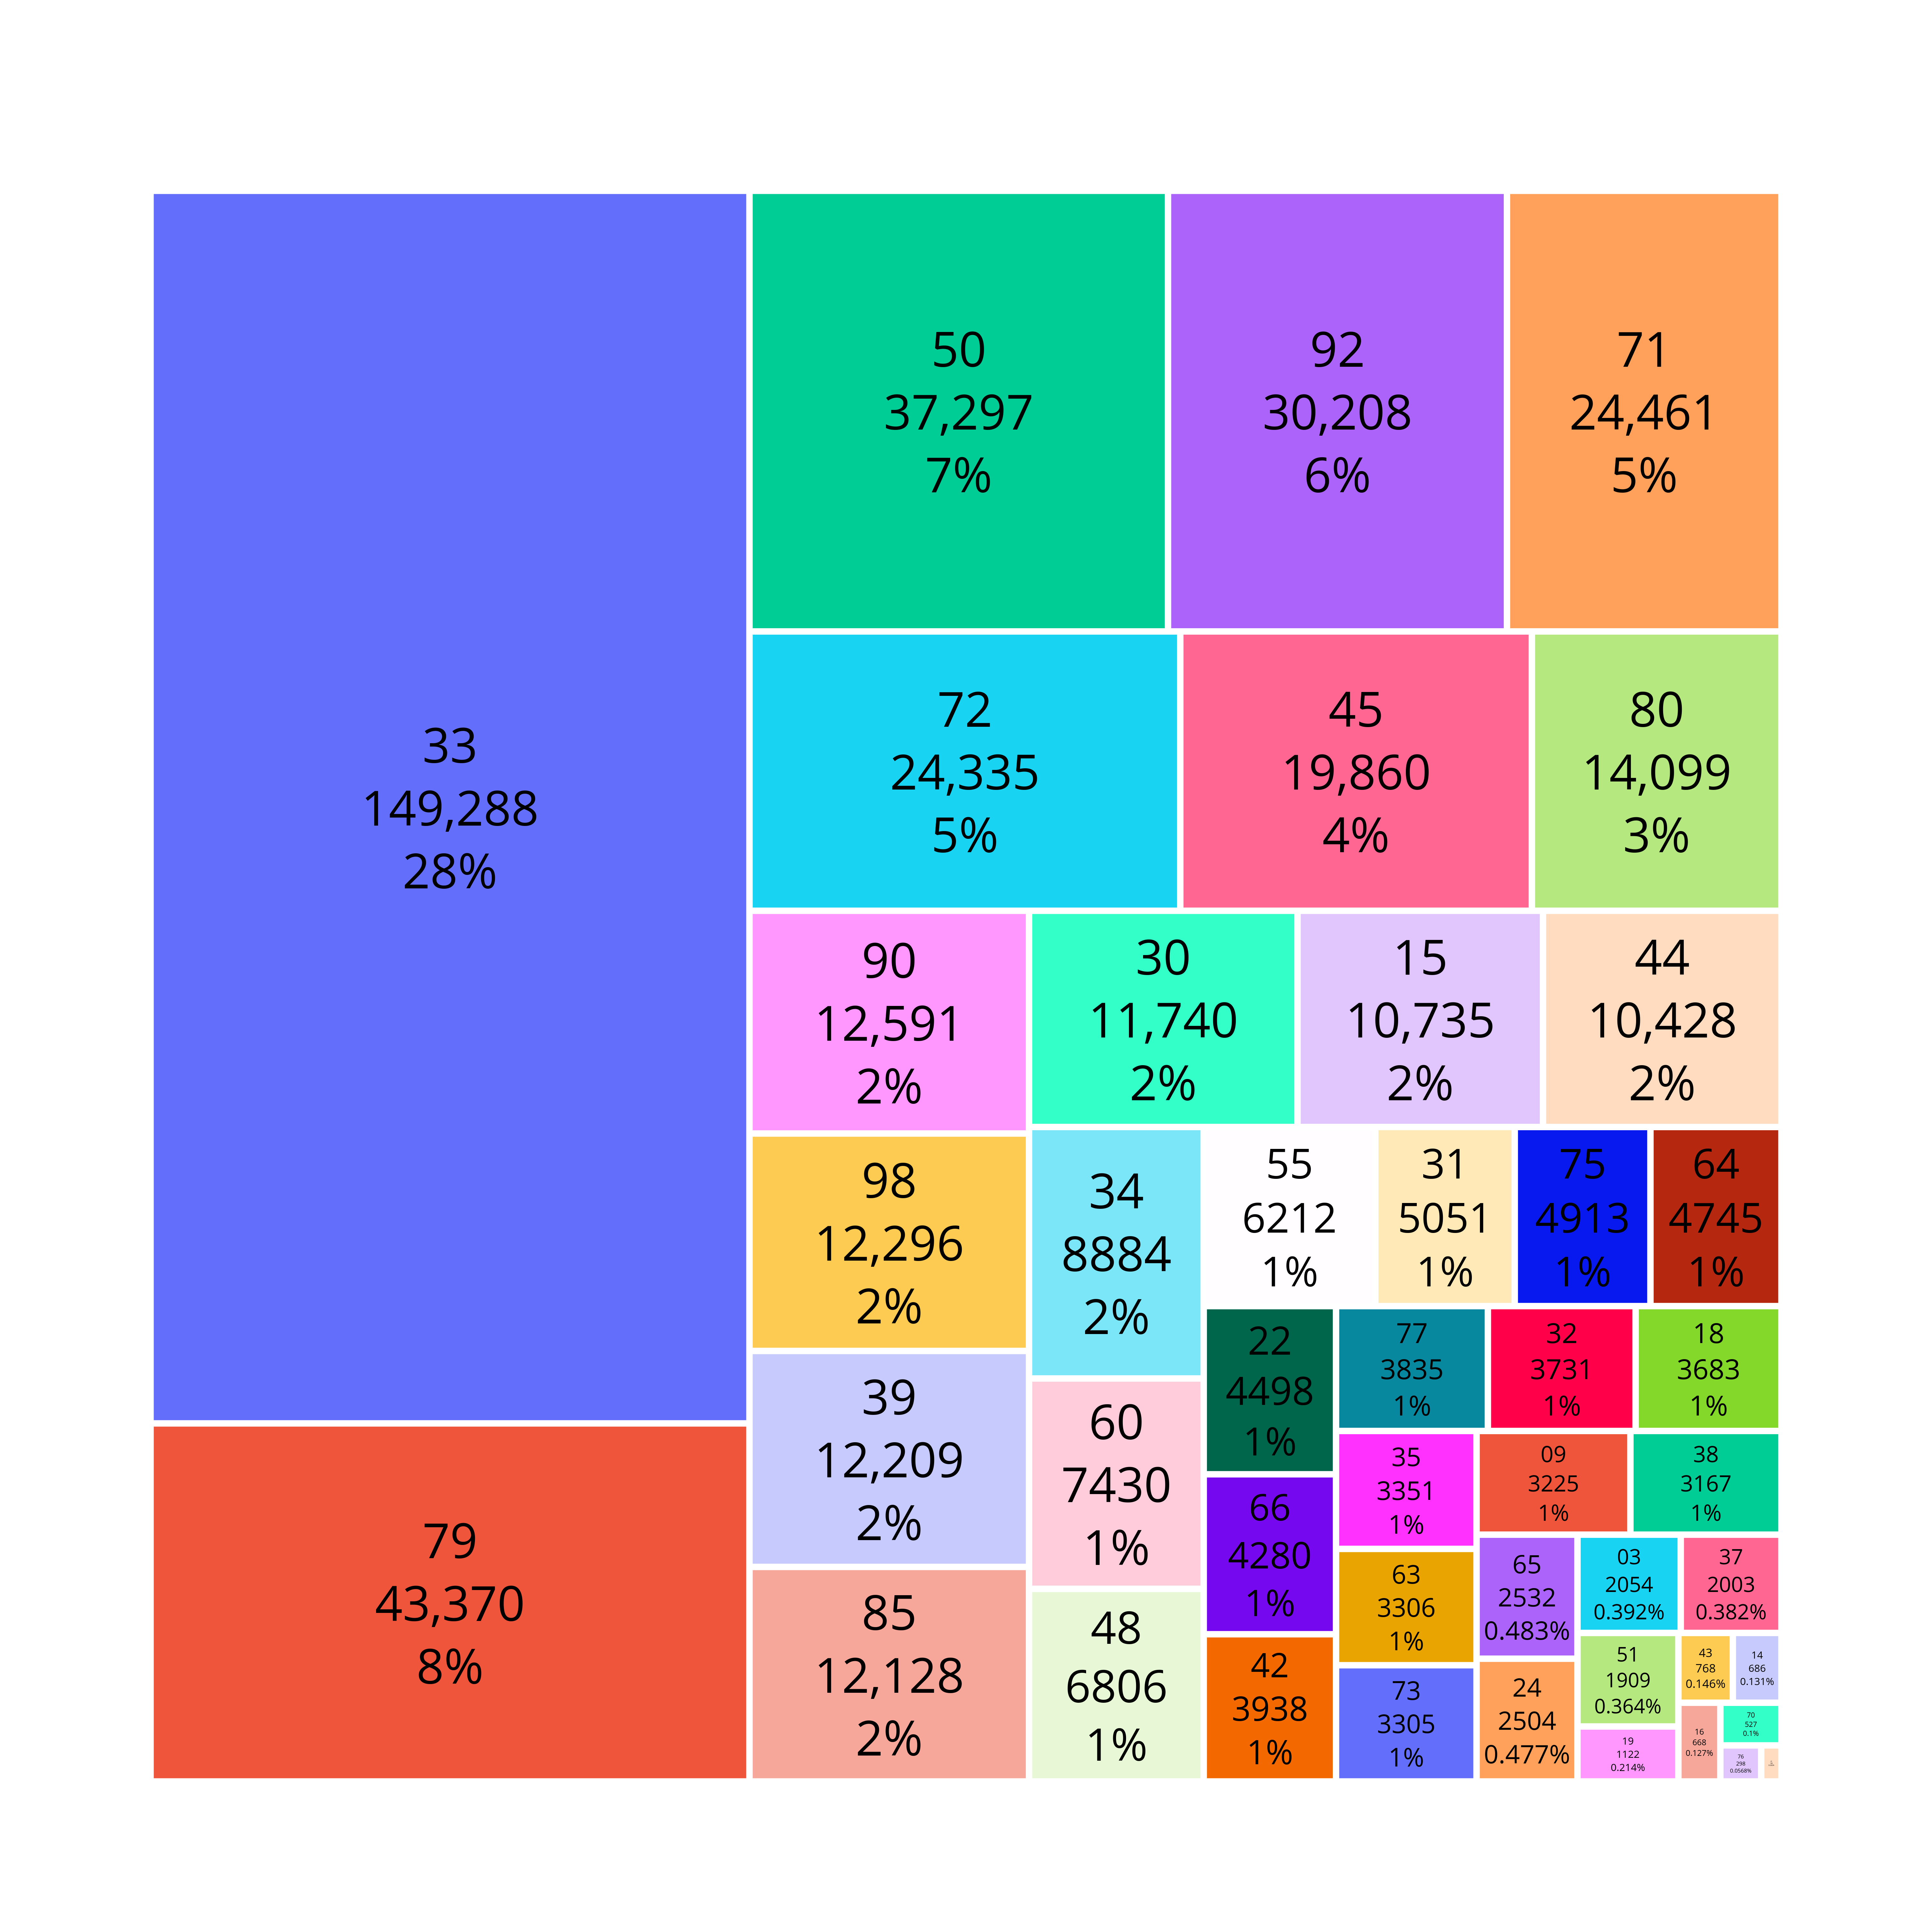
\includegraphics[width=\textwidth]{imagens/treemap_contratos_adir.png}
		\caption{Distribuição do número de ajustes diretos em regime geral, por divisão de CPV.}
		\label{fig:adcpv}
	\end{minipage}
	\hfill
	\begin{minipage}[t]{0.49\textwidth}
		\centering
		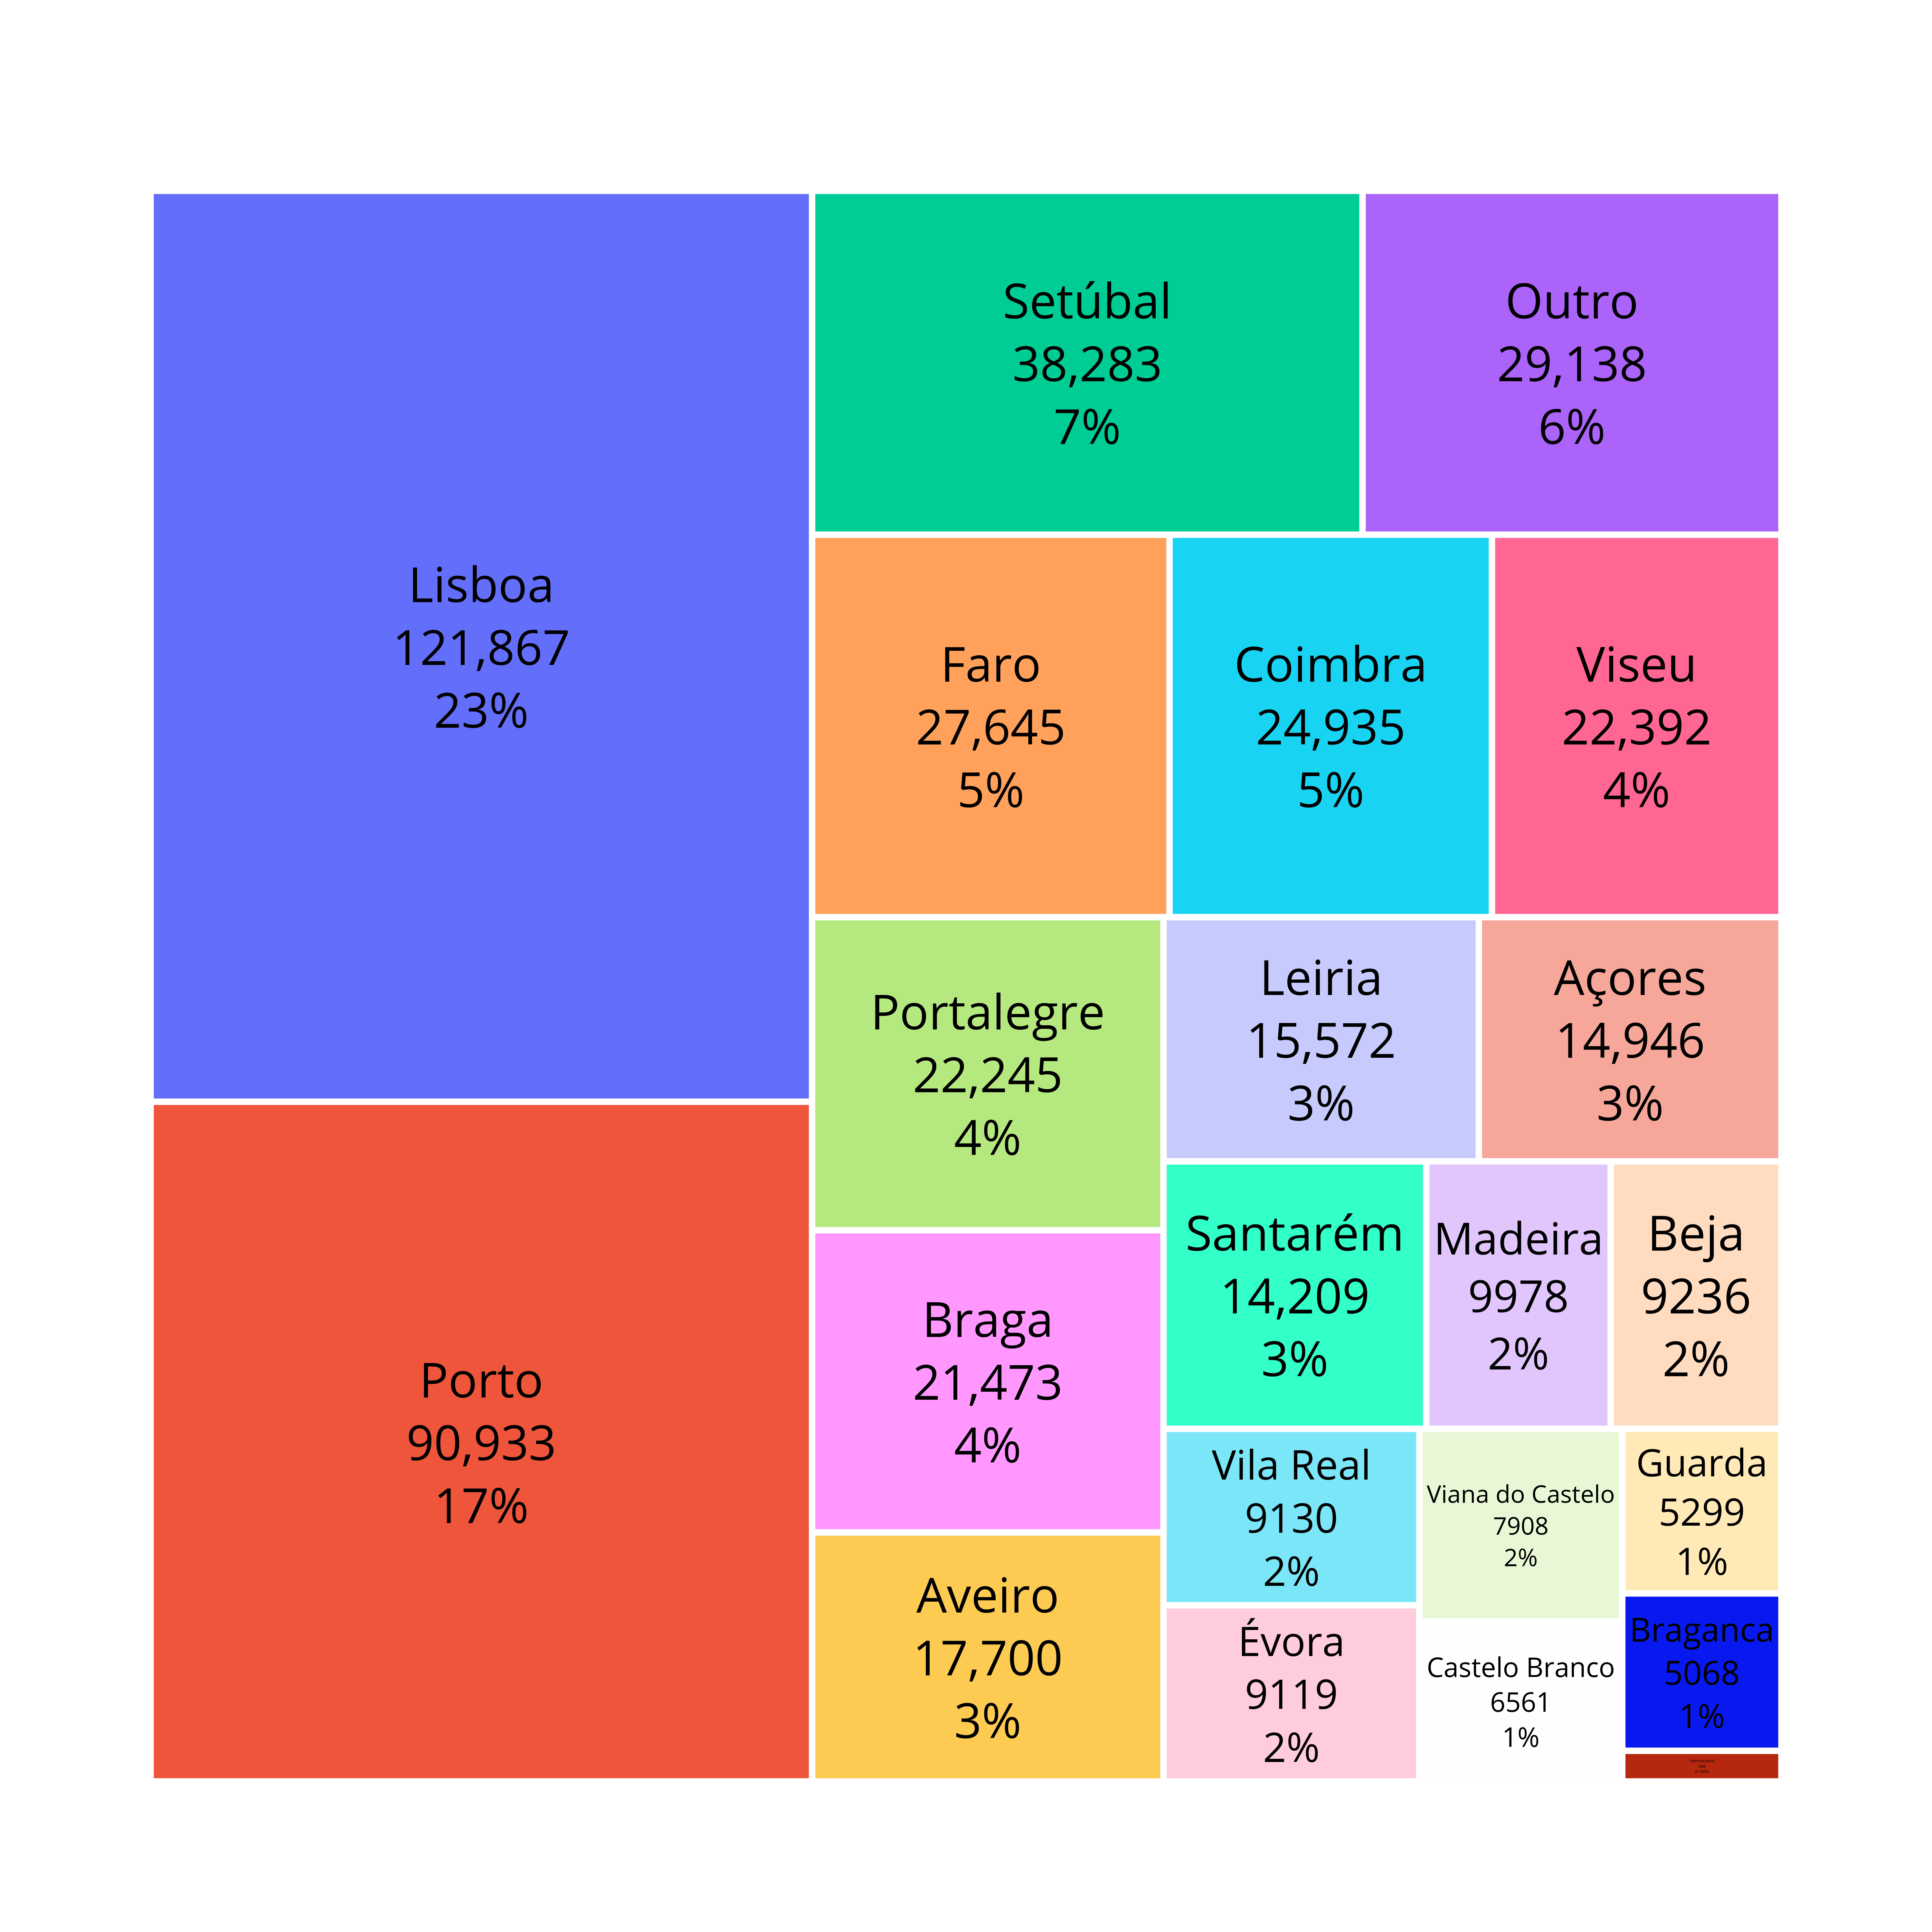
\includegraphics[width=\textwidth]{imagens/treemap_distritos_adir.png}
		\caption{Distribuição do número de ajustes diretos em regime geral, por distrito.}
		\label{fig:adloc}
	\end{minipage}
	
\end{figure}
\clearpage


%\subsection{Exemplo ilustrativo: Contratos referentes à área da saúde}
%
%\begin{figure}[H]
%	\begin{minipage}{0.33\linewidth}
%		%\centering  % redundant
%		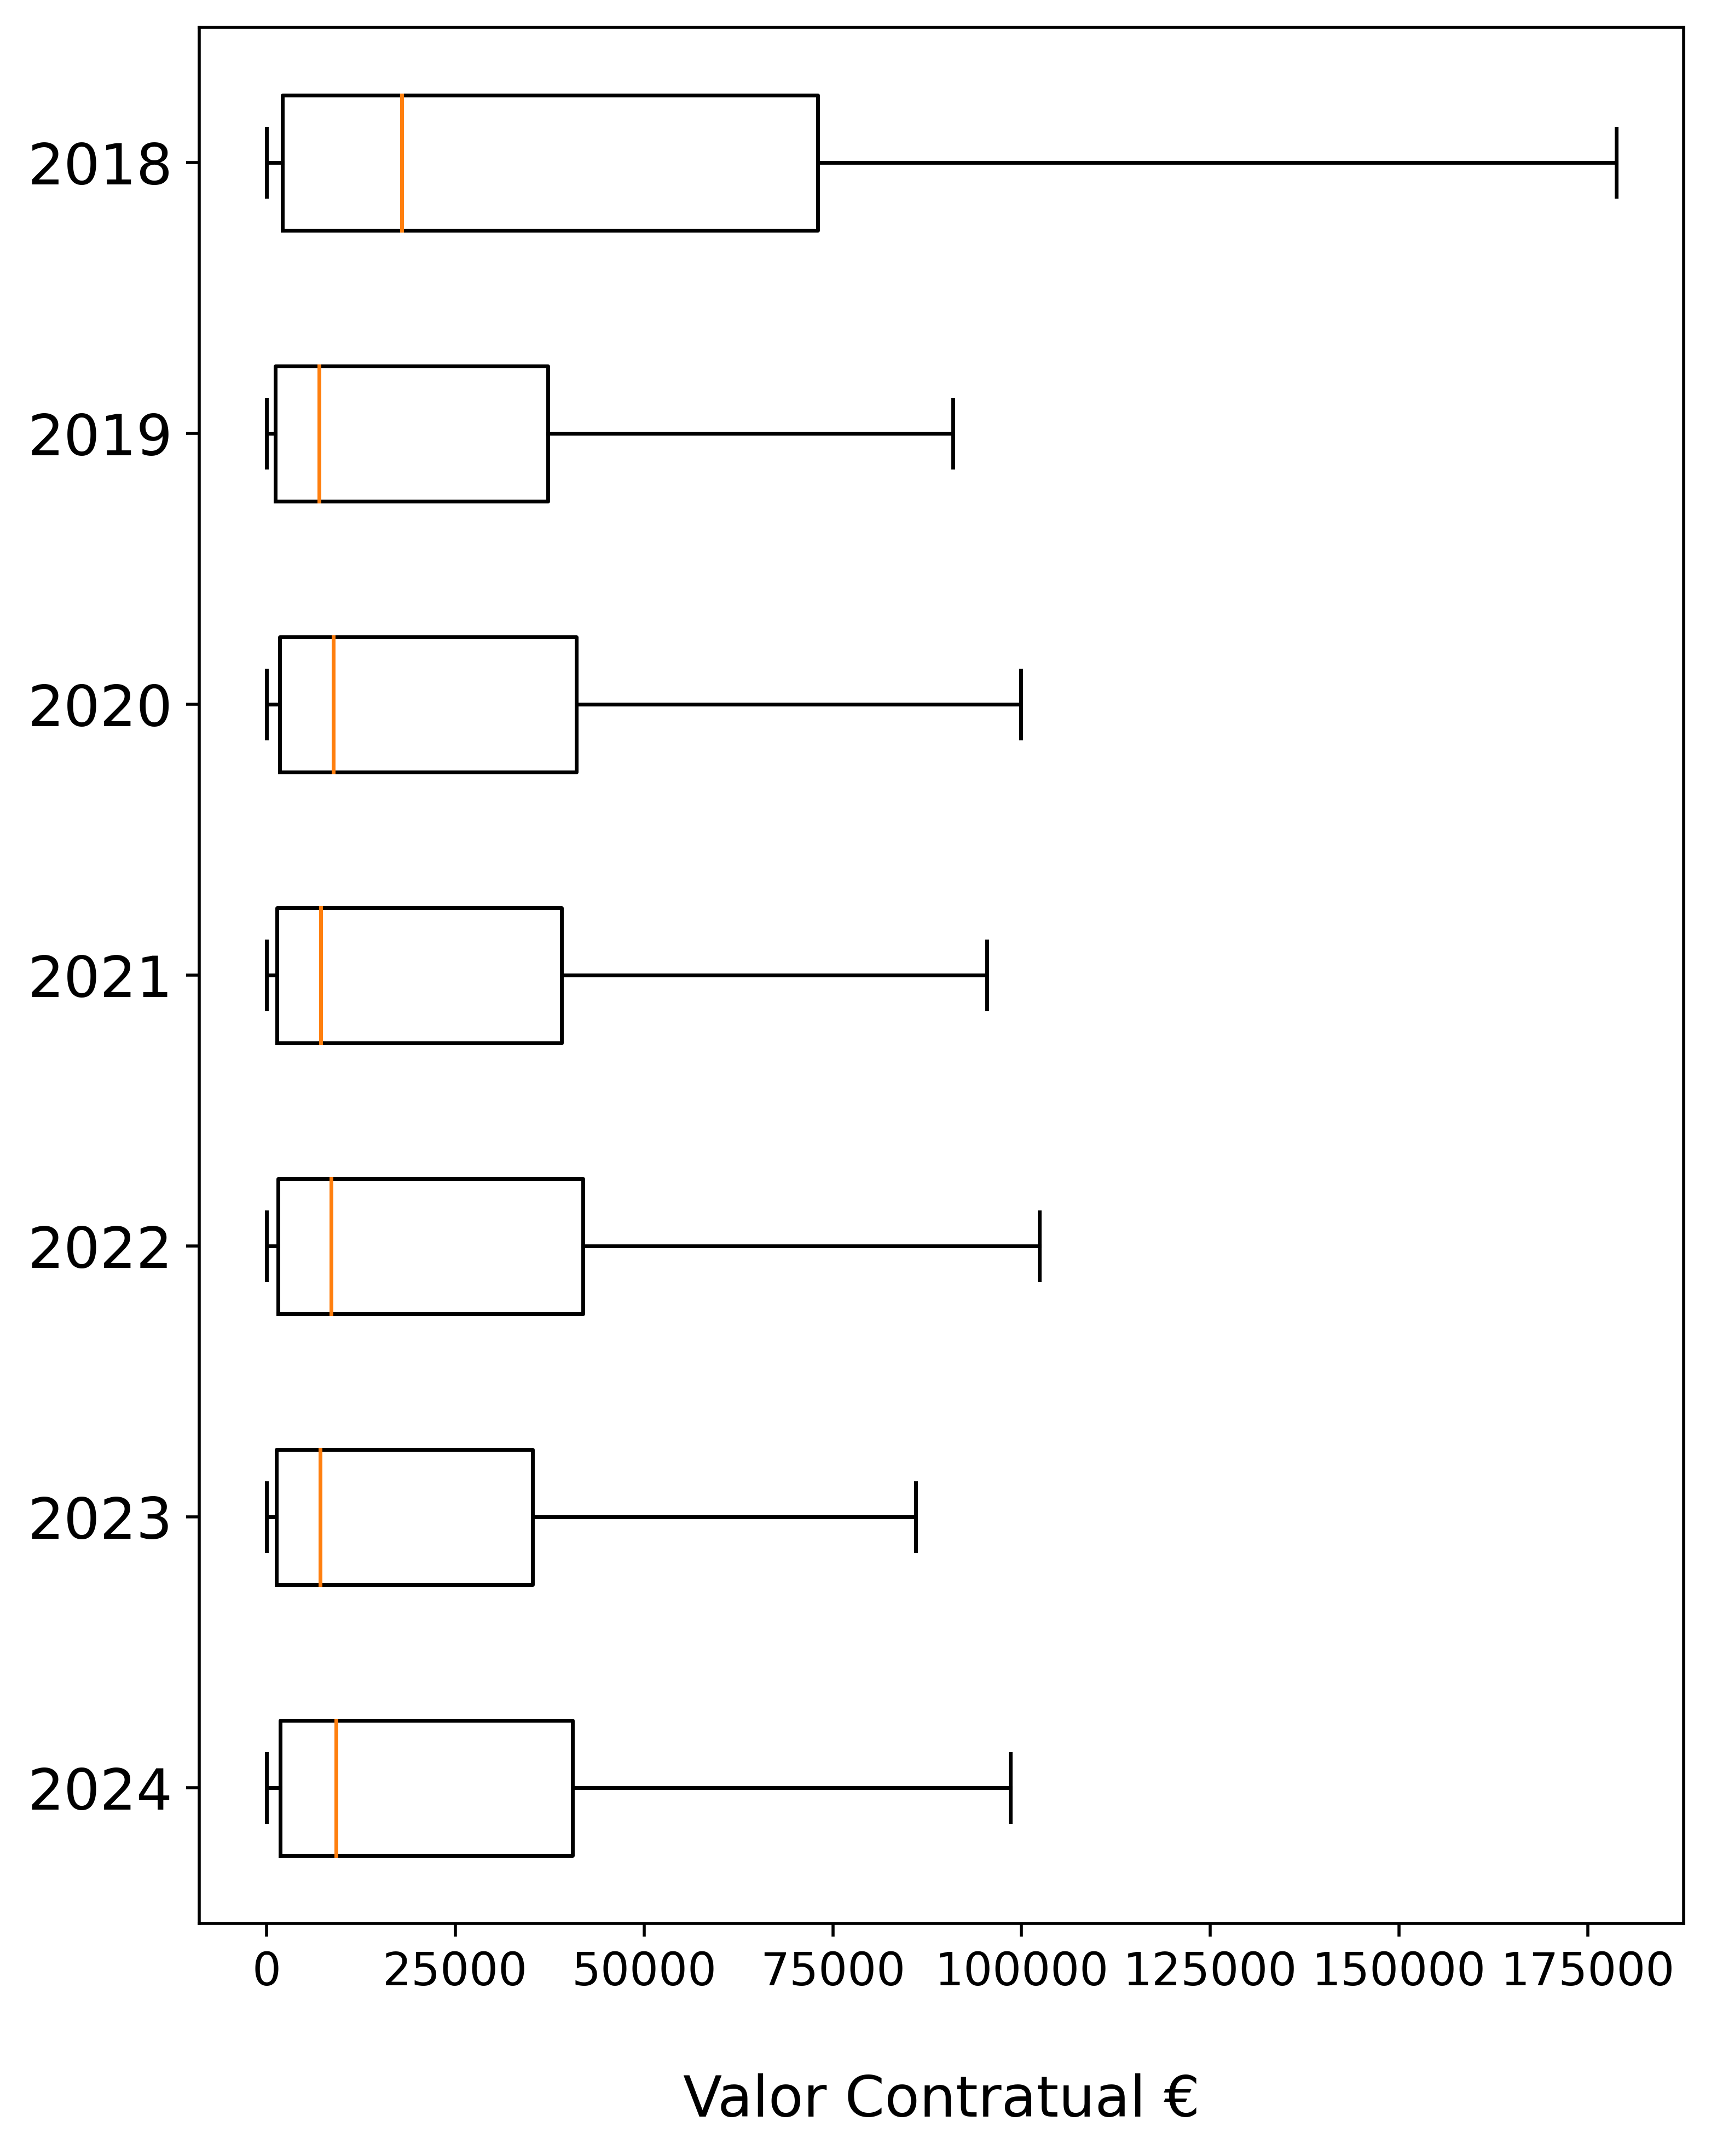
\includegraphics[width=\textwidth]{imagens/cp_anos_33_v1.png}
%		\caption{Boxplot dos preços contratuais para concursos públicos referentes à área da saúde desde 2018 até 2024}
%	\end{minipage}%
%	\hfill% not: "\hspace{0.5cm}"
%	\begin{minipage}{0.33\linewidth}
%		%\centering  % redundant
%		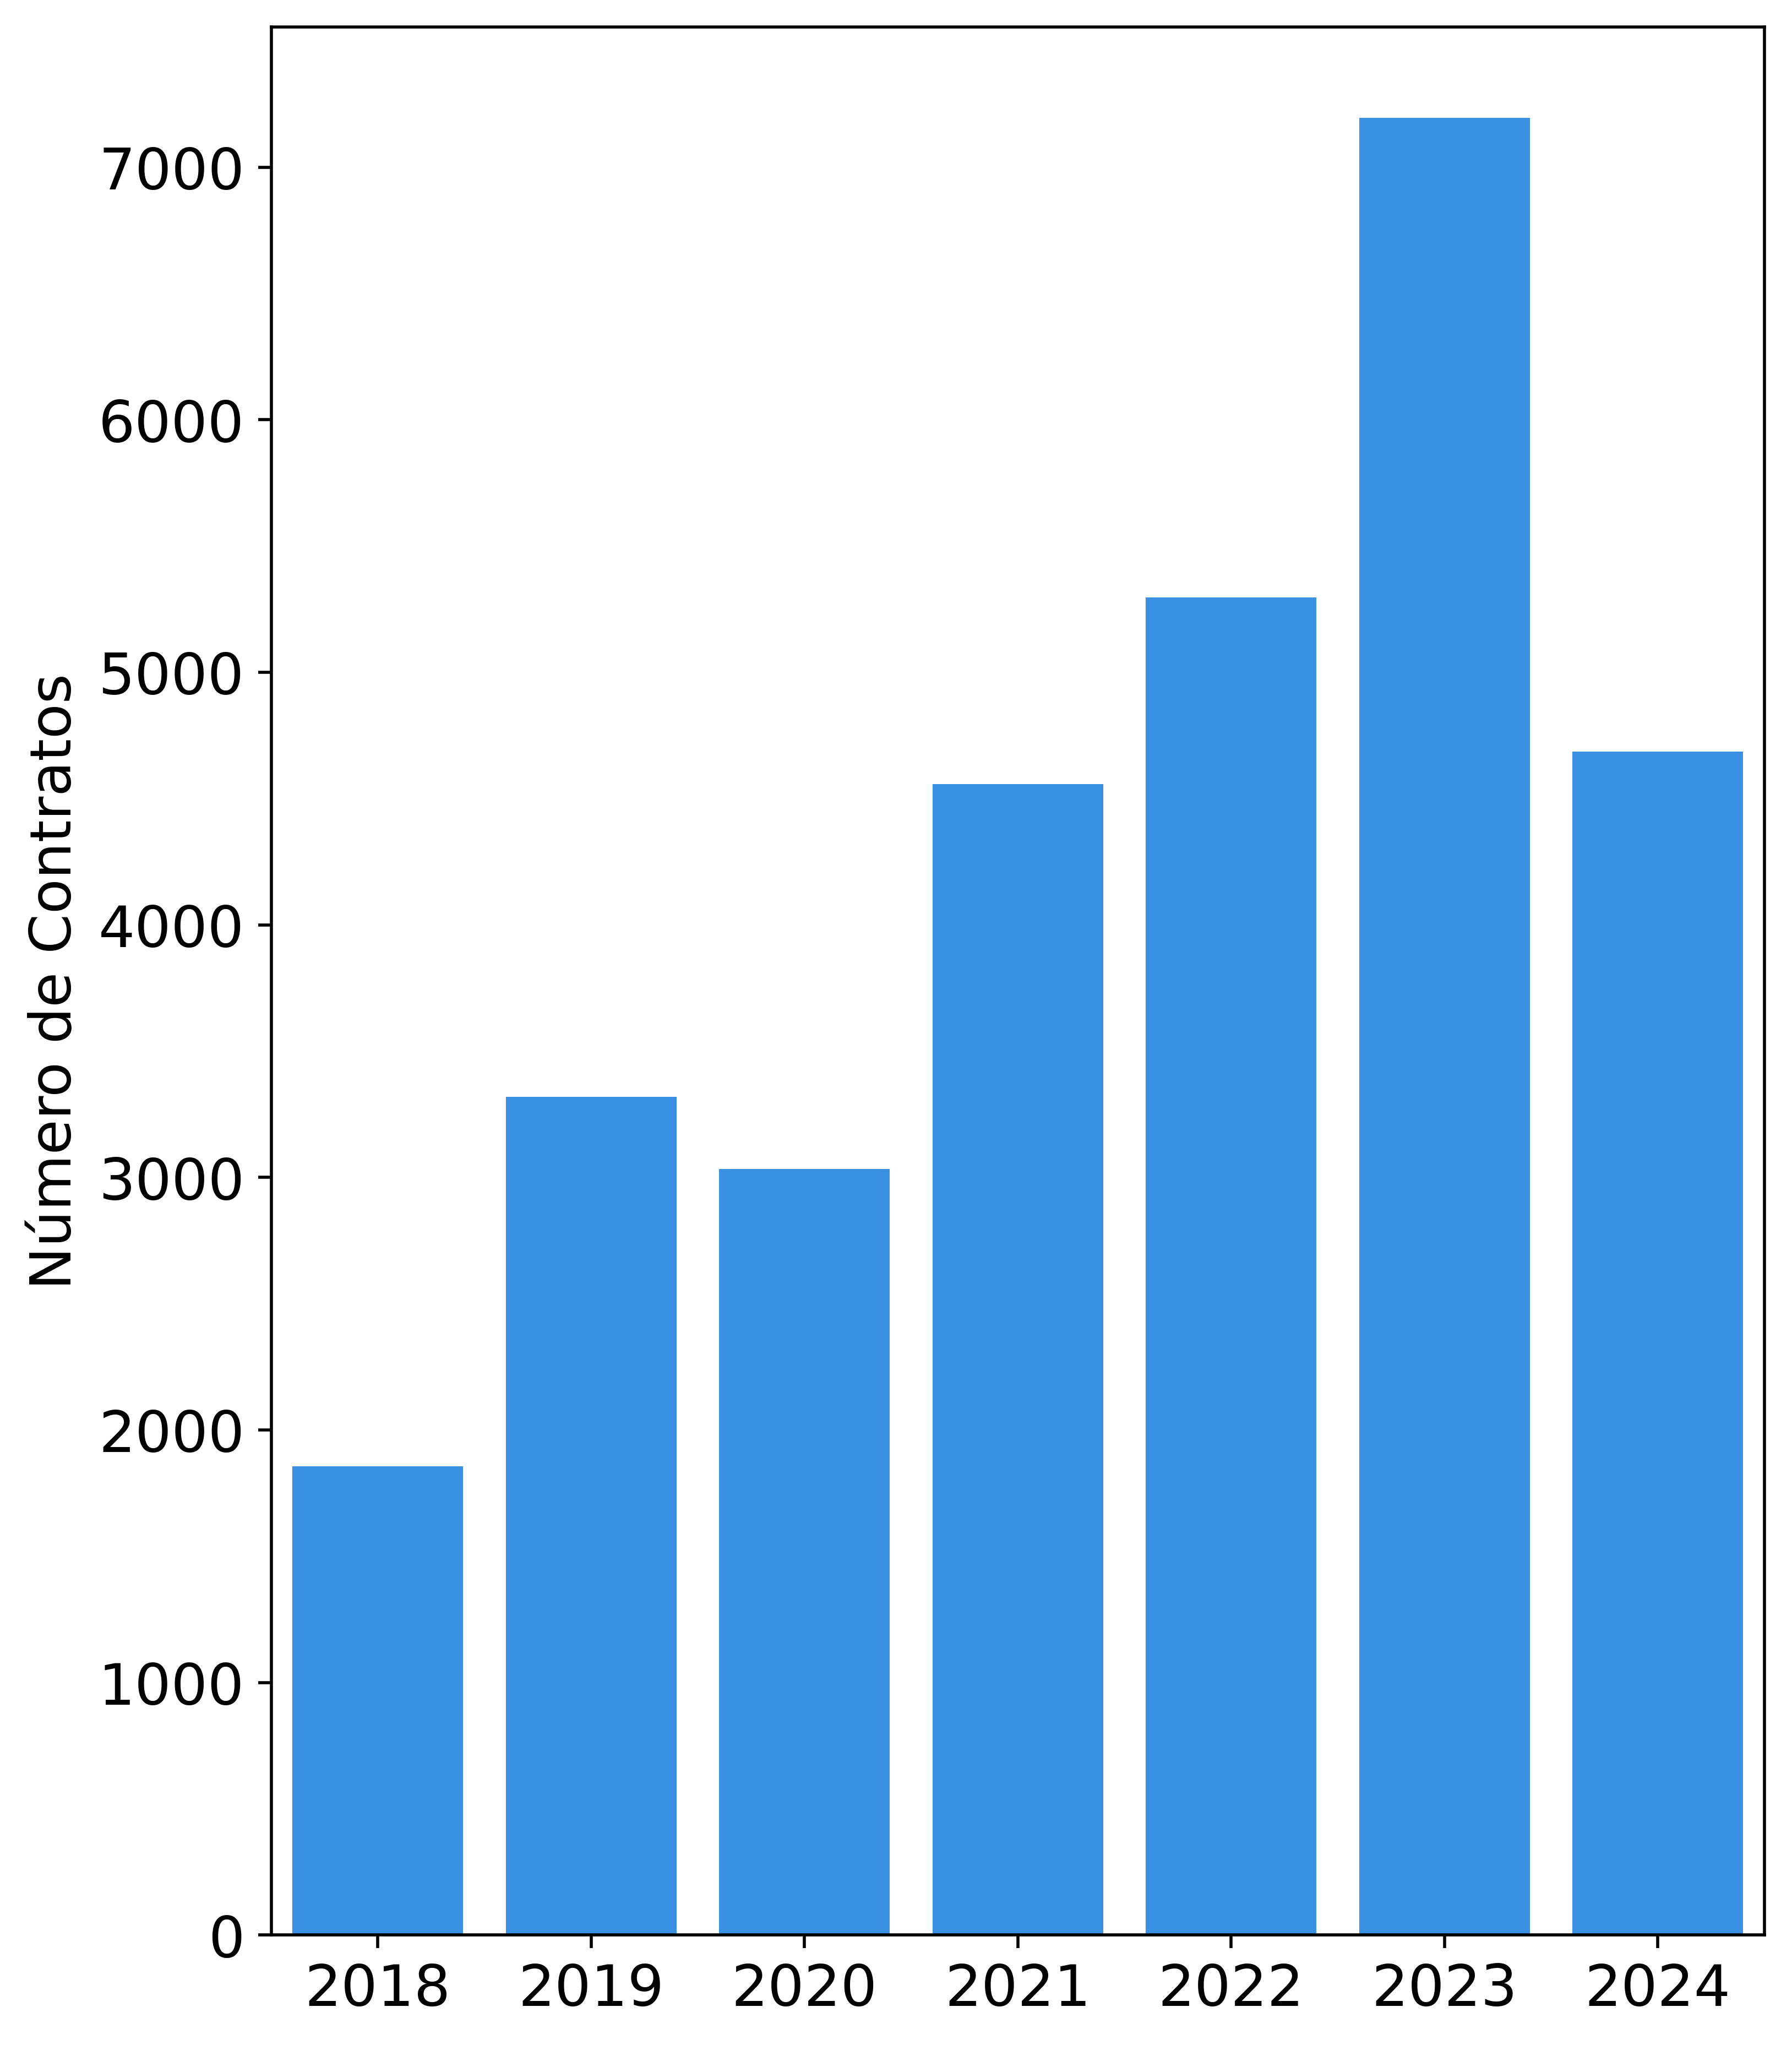
\includegraphics[width=\textwidth]{imagens/cp_anos_33_v2.png}
%		\caption{Número de concursos públicos celebrados referentes à área da saúde desde 2018 até 2024}
%	\end{minipage}%
%	\hfill% not: "\hspace{0.5cm}"
%	\begin{minipage}{0.33\linewidth}
%		%\centering  % redundant
%		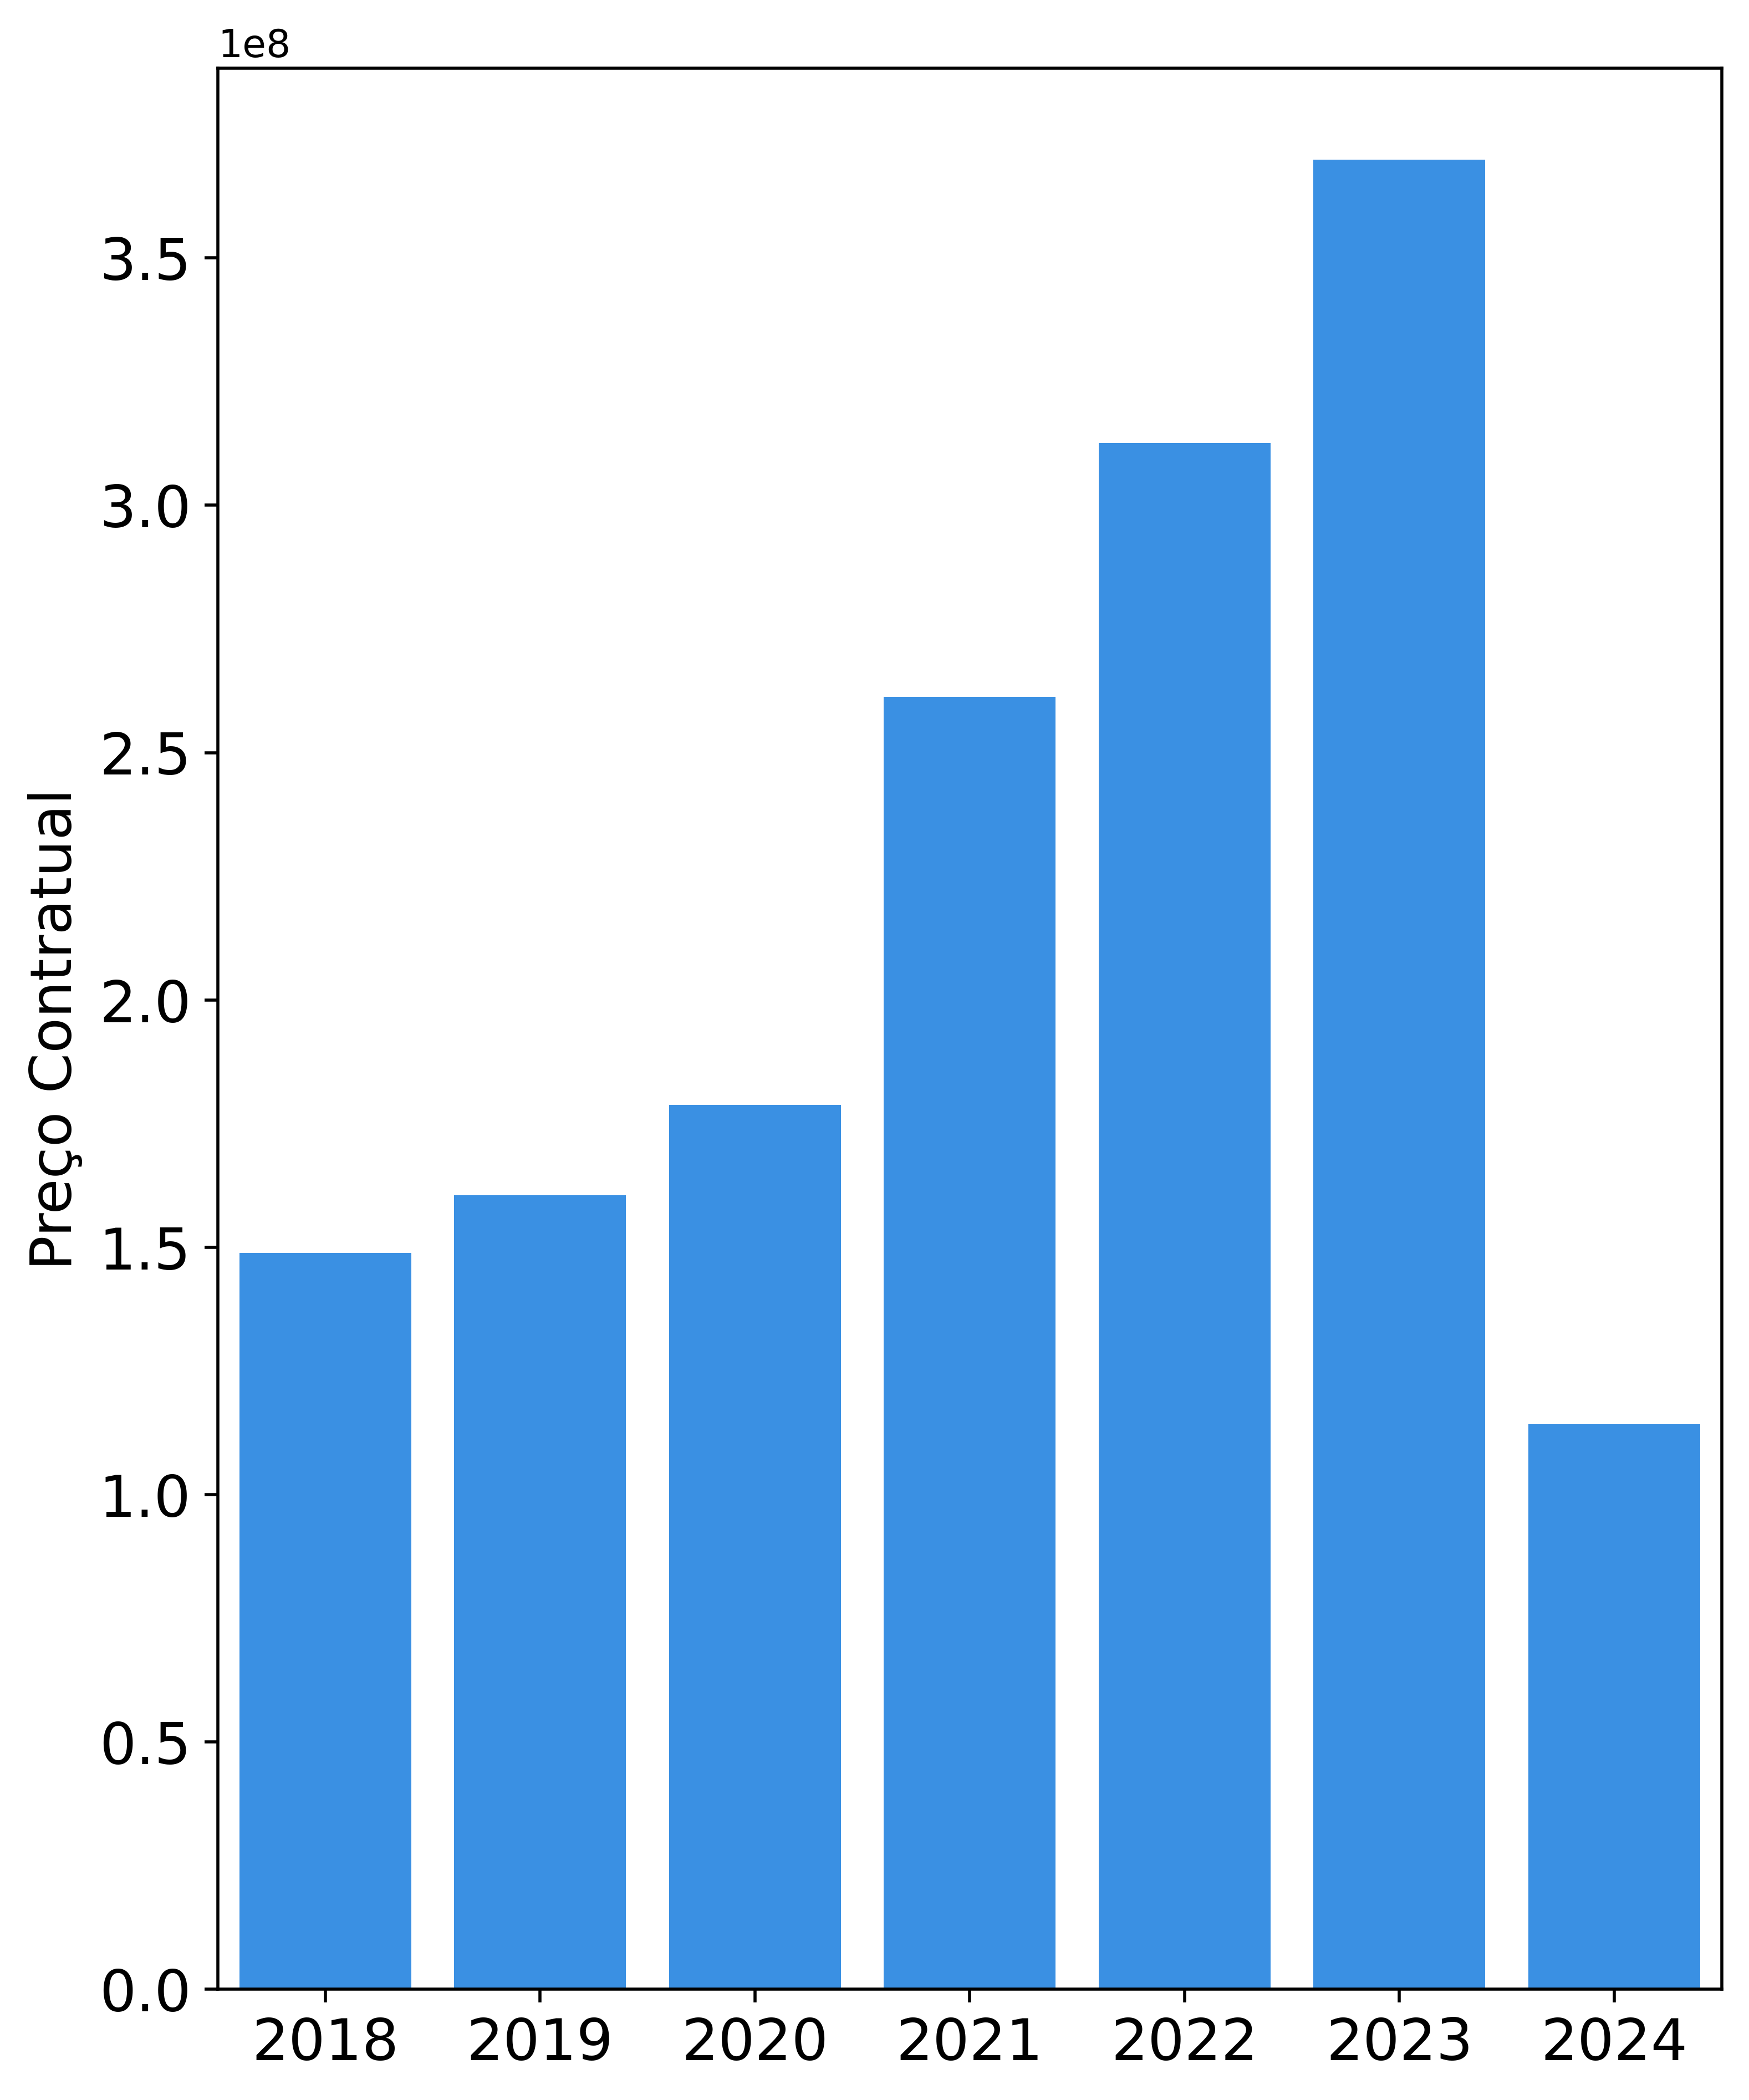
\includegraphics[width=\textwidth]{imagens/cp_anos_33_v3.png}
%		\caption{Montante total adjudicada a contratos públicos celebrados referentes à área da saúde desde 2018 até 2024}
%	\end{minipage}
%\end{figure}
%
%
%
%\begin{figure}[H]
%	\begin{minipage}{0.33\linewidth}
%		%\centering  % redundant
%		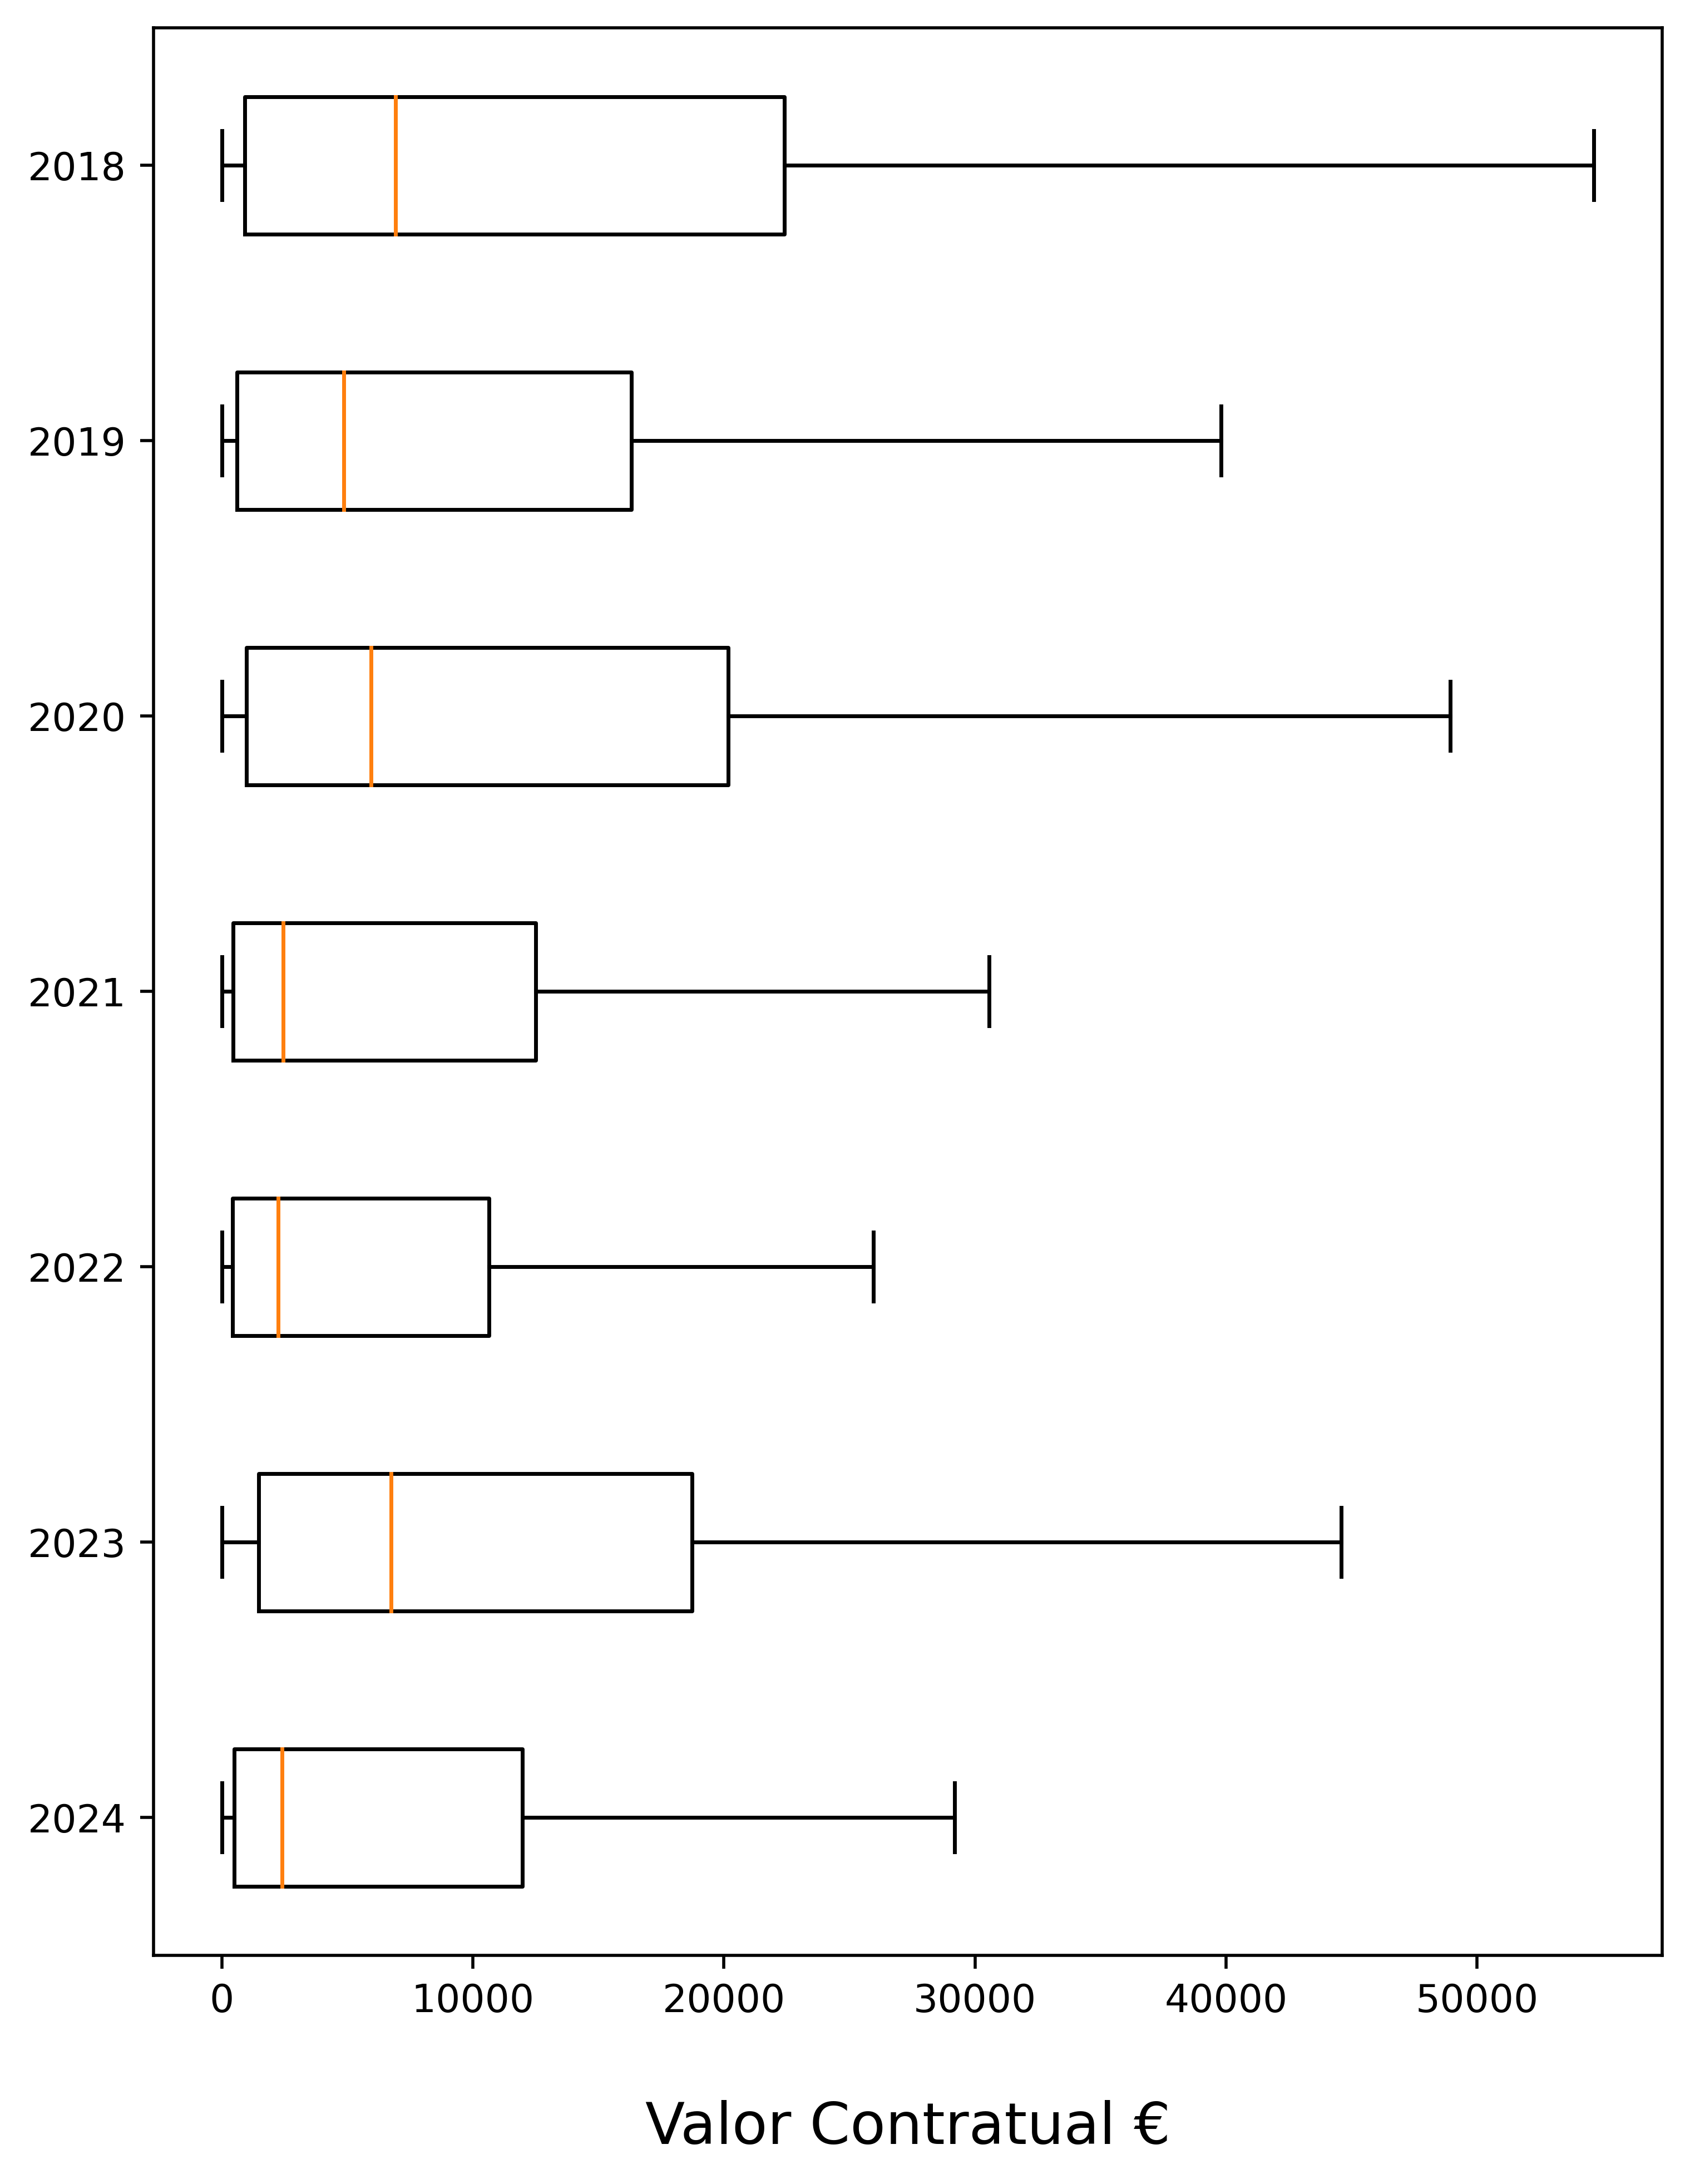
\includegraphics[width=\textwidth]{imagens/ajdir_anos33_v1.png}
%		\caption{Boxplot dos preços contratuais para ajustes diretos em regime geral referentes à área da saúde desde 2018 até 2024}
%	\end{minipage}%
%	\hfill% not: "\hspace{0.5cm}"
%	\begin{minipage}{0.33\linewidth}
%		%\centering  % redundant
%		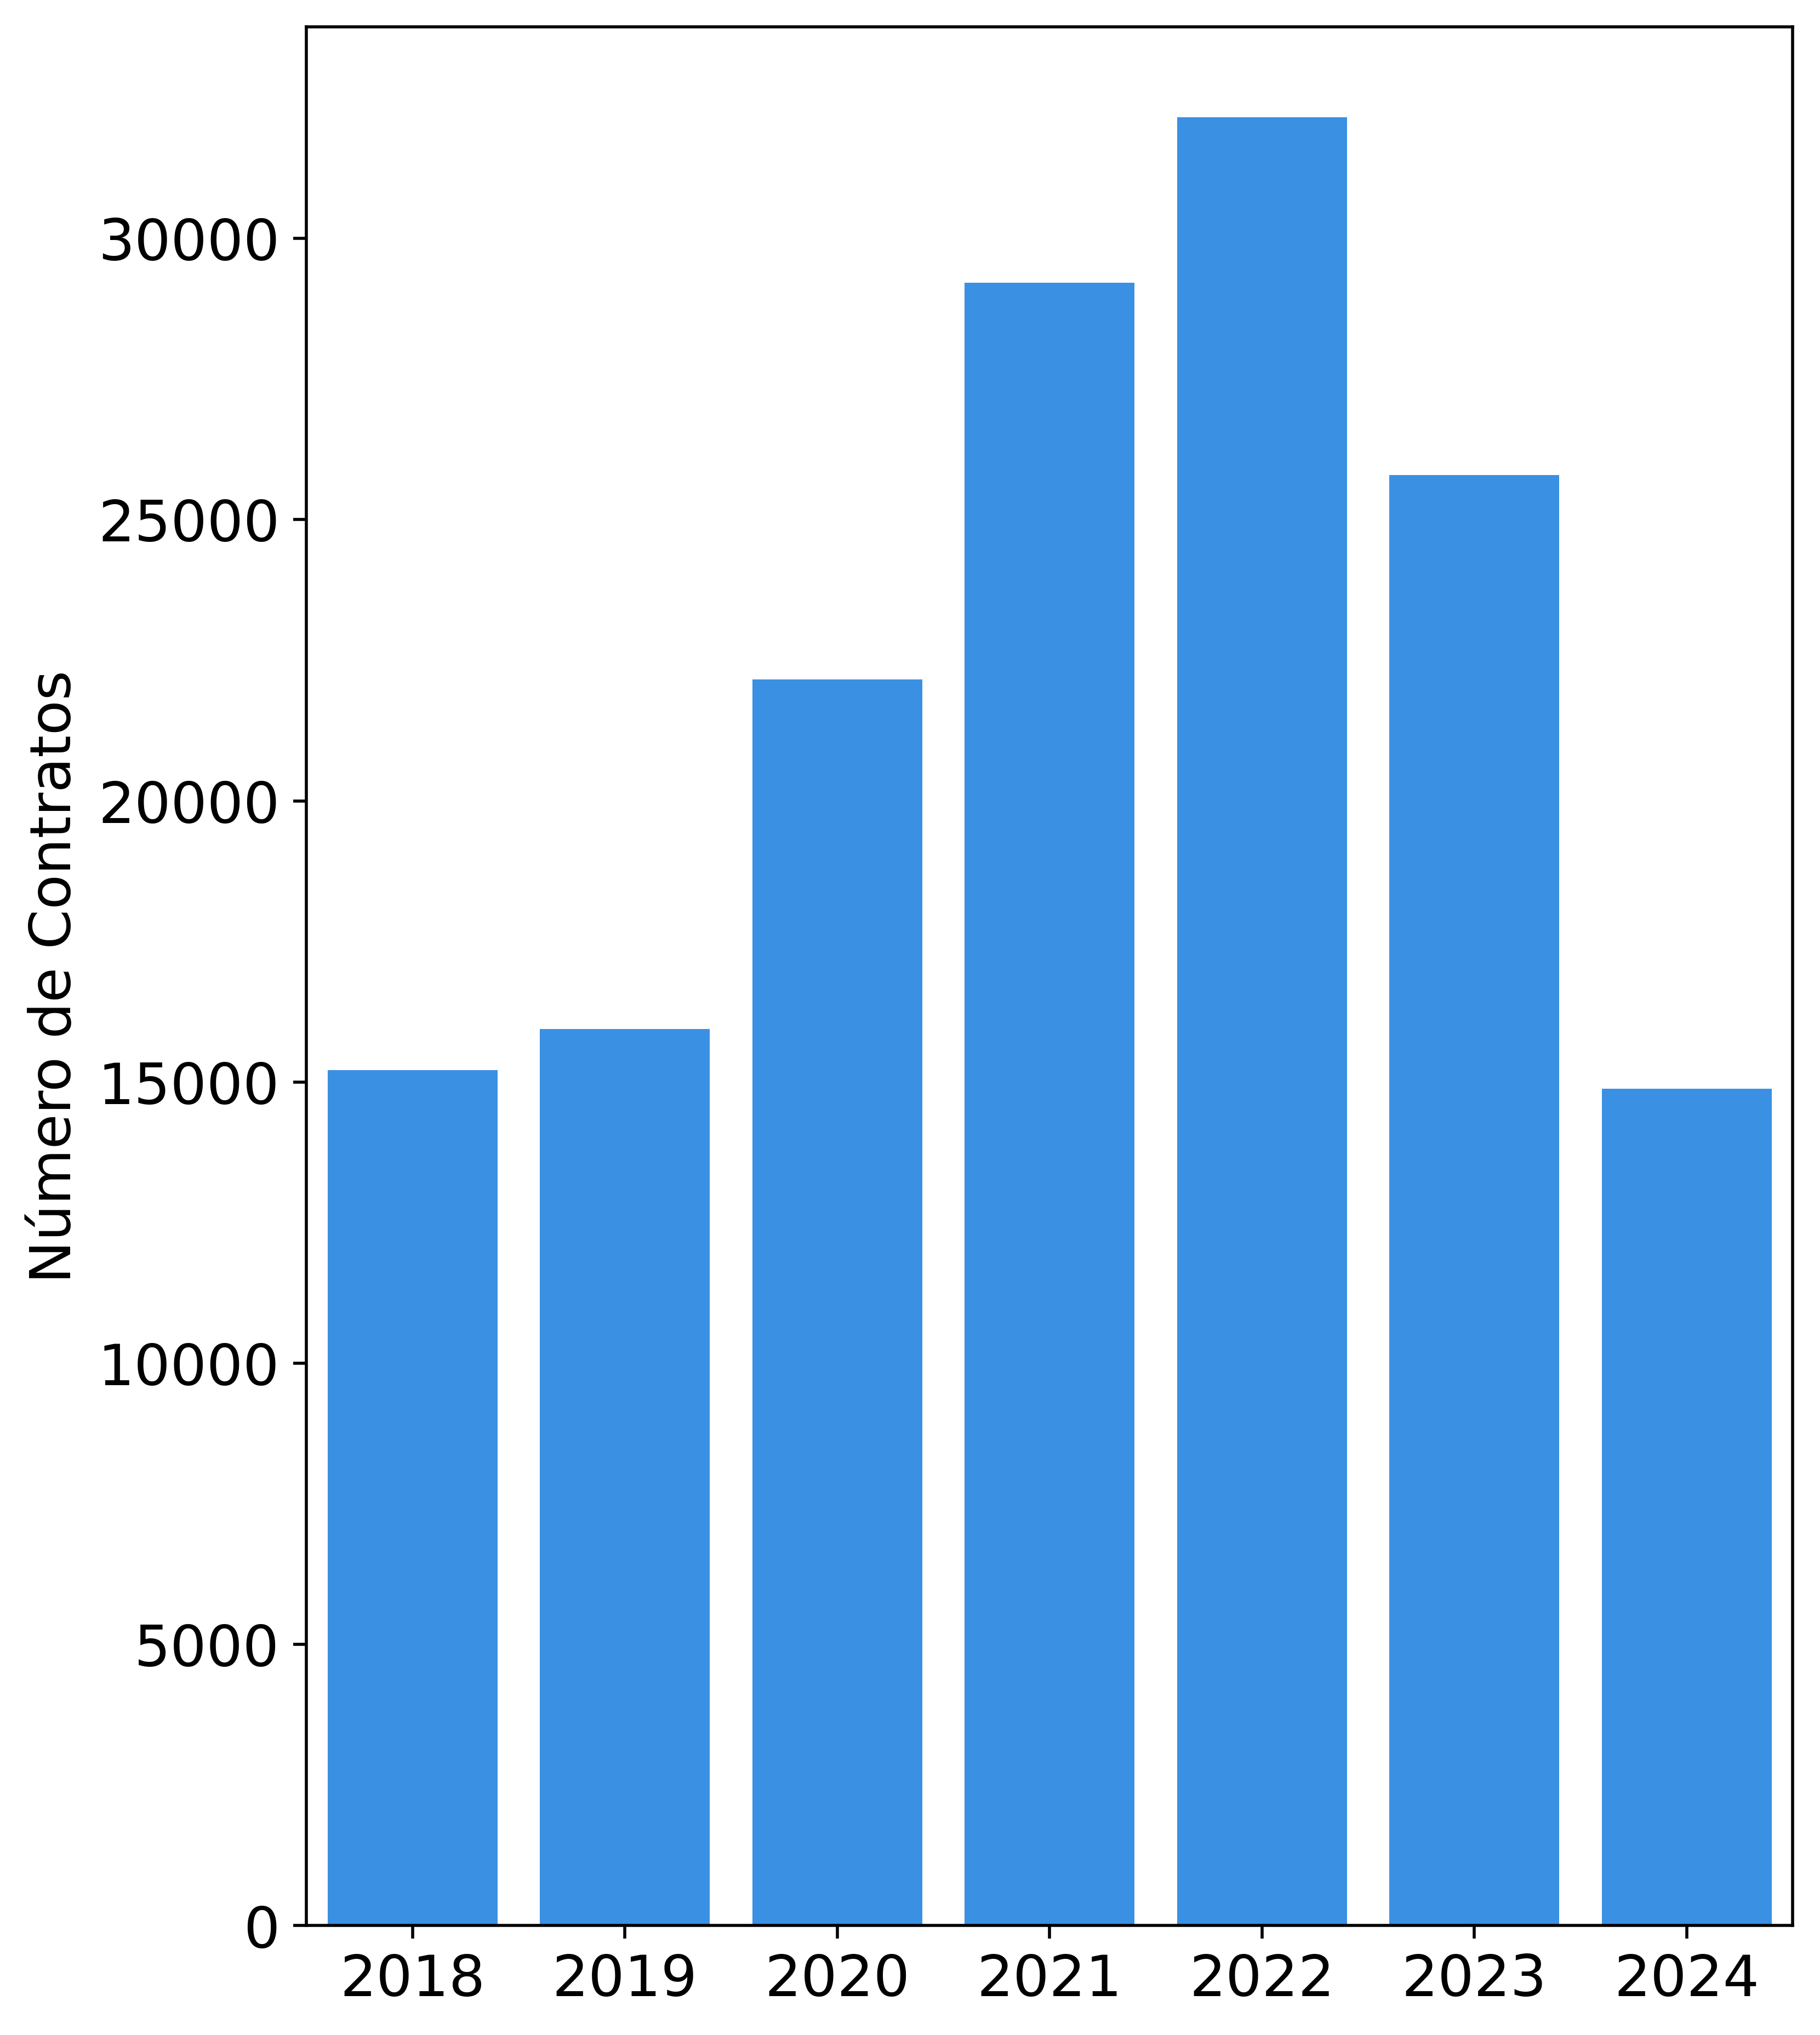
\includegraphics[width=\textwidth]{imagens/ajdir_anos33_v2.png}
%		\caption{Número de ajustes diretos em regime geral celebrados referentes à área da saúde desde 2018 até 2024}
%	\end{minipage}%
%	\hfill% not: "\hspace{0.5cm}"
%	\begin{minipage}{0.33\linewidth}
%		%\centering  % redundant
%		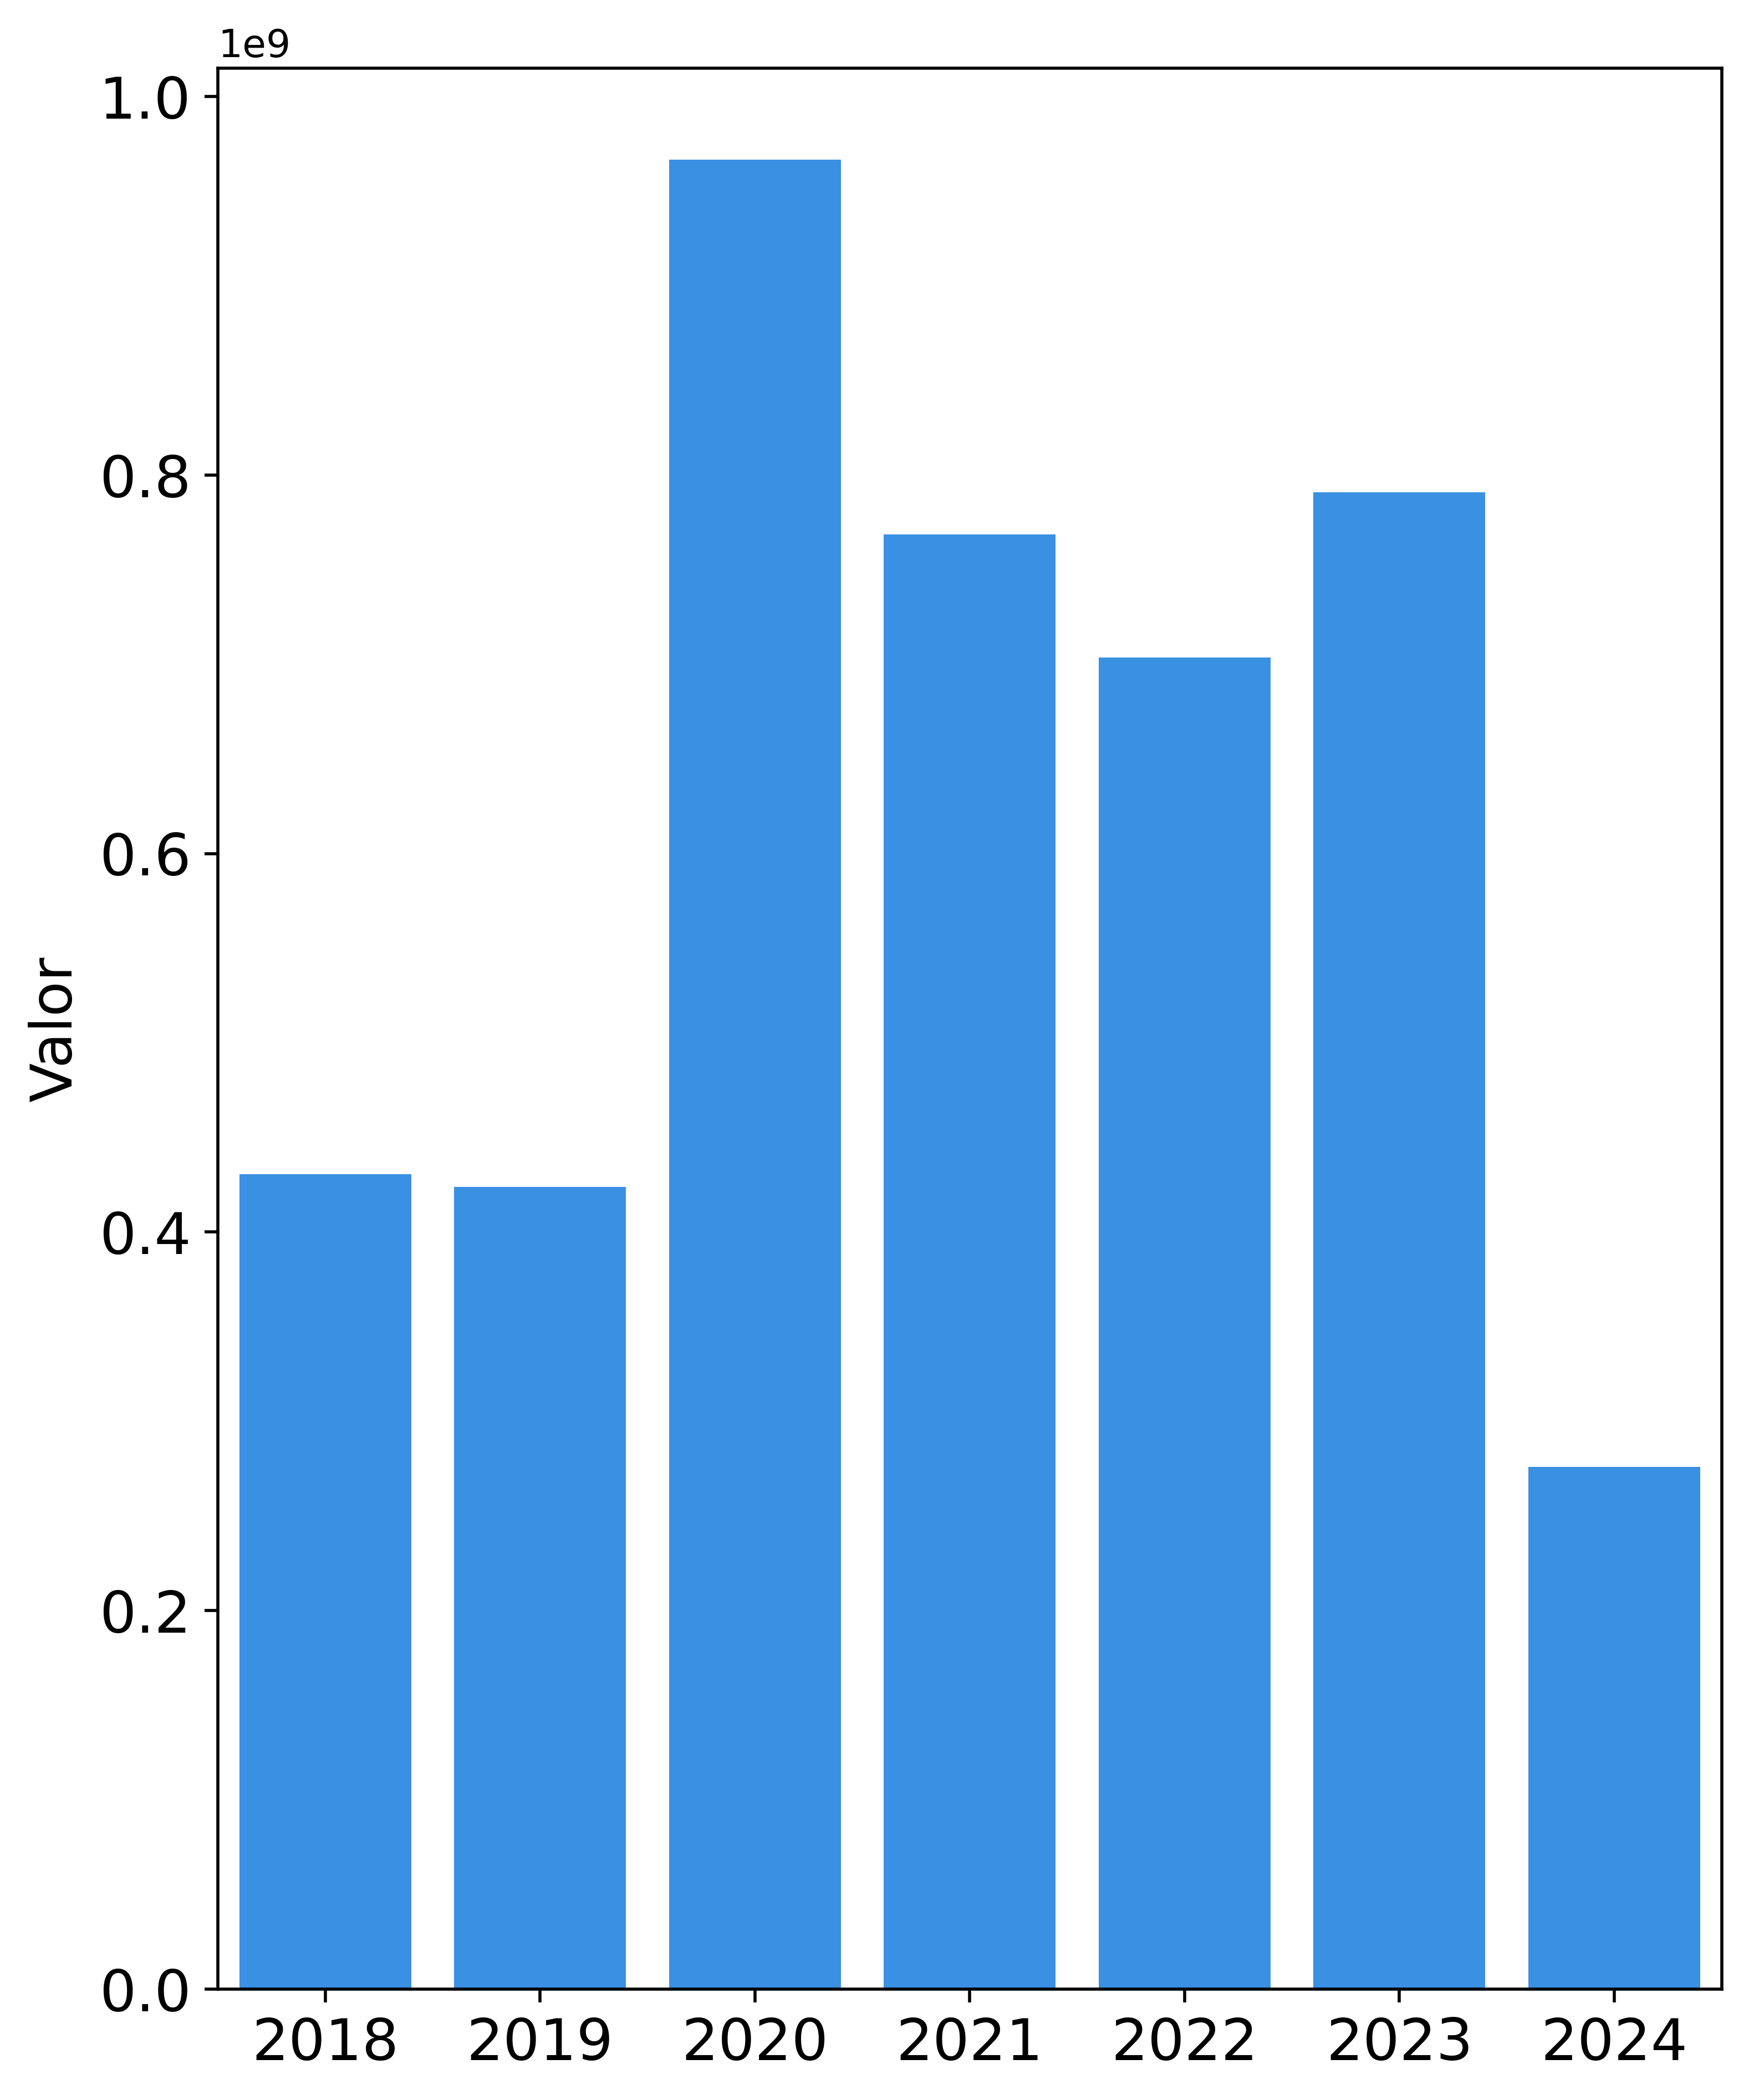
\includegraphics[width=\textwidth]{imagens/ajdir_anos33_v3.png}
%		\caption{Montante total adjudicada a ajustes diretos em regime geral celebrados referentes à área da saúde desde 2018 até 2024}
%	\end{minipage}
%\end{figure}
